%%%%%%%%%%%%%%%%%%%%%%%%%%%%%%%%%%%%%%%%%%%%%%%%%%%%%%%%%%%%%%%%%%%%%%%%%%%%%%%%
% Preámbulo                                                                    %
%%%%%%%%%%%%%%%%%%%%%%%%%%%%%%%%%%%%%%%%%%%%%%%%%%%%%%%%%%%%%%%%%%%%%%%%%%%%%%%%

\documentclass[11pt,a4paper,titlepage,oneside]{report}
%%% RELACIÓN DE VARIABLES A PERSONALIZAR %%%
%\def\lingua{gal}
\def\lingua{esp} % descomenta esta liña se redactarás a memoria en español
%\def\lingua{eng} % descomenta esta liña se redactarás a memoria en inglés
\def\nome{Adrián García Vázquez}                             % substitúe aquí o teu nome
\def\nomedirectorA{Manuel Álvarez Díaz}              % substitúe aquí o nome de quen dirixe
%\def\nomedirectorB{Outro Nome Completo}             % duplica esta liña máis veces se o precisas, cambiando
                                                     % a letra final (A, B, C, D...): úsanse na portada.tex
\def\titulo{Aplicación para la Gestión de Emergencias} % substitúe aquí o título do teu TFG
%\def\mencion{NOME DA MENCIÓN}                        % descomenta a mención correspondente
%\def\mencion{COMPUTACIÓN}
\def\mencion{ENXEÑARÍA DO SOFTWARE}
%\def\mencion{ENXEÑARÍA DE COMPUTADORES}
%\def\mencion{SISTEMAS DE INFORMACIÓN}
%\def\mencion{TECNOLOXÍAS DA INFORMACIÓN}

\def\renomearcadros{si} % comenta esta liña se redactas a memoria en galego e prefires que
                         % "tablas" e "índice de tablas" se renomeen a 
                         % "cuadros" e o "índice de cuadros" respectivamente


\usepackage{estilo}

% Lista de paquetes potencialmente interesantes (uso baixo demanda)

% \usepackage{alltt}       % proporciona o entorno alltt, semellante a verbatim pero que respecta comandos
% \usepackage{enumitem}    % permite personalizar os entornos de lista
\usepackage{eurosym}    % proporciona o comando \euro
% \usepackage{float}       % permite máis opcións para controlar obxectos flotantes (táboas, figuras)
% \usepackage{hhline}      % permite personalizar as liñas horizontais en arrays e táboas
\usepackage{longtable}   % permite construir táboas que ocupan máis dunha páxina
% \usepackage{lscape}      % permite colocar partes do documento en orientación apaisada
% \usepackage{moreverb}    % permite personalizar o entorno verbatim
% \usepackage{multirow}    % permite crear celdas que ocupan varias filas da mesma táboa
% \usepackage{pdfpages}    % permite insertar ficheiros en PDF no documento
% \usepackage{rotating}    % permite diferentes tipos de rotacións para figuras e táboas
% \usepackage{subcaption}  % permite a inclusión de varias subfiguras nunha figura
% \usepackage{tabu}        % permite táboas flexibles
% \usepackage{tabularx}    % permite táboas con columnas de anchura determinada

\usepackage[babel=true]{microtype}

%%%%%%%%%%%%%%%%%%%%%%%%%%%%%%%%%%%%%%%%%%%%%%%%%%%%%%%%%%%%%%%%%%%%%%%%%%%%%%%%
% Corpo                                                                        %
%%%%%%%%%%%%%%%%%%%%%%%%%%%%%%%%%%%%%%%%%%%%%%%%%%%%%%%%%%%%%%%%%%%%%%%%%%%%%%%%

\begin{document}

 %%%%%%%%%%%%%%%%%%%%%%%%%%%%%%%%%%%%%%%%
 % Preliminares do documento            %
 %%%%%%%%%%%%%%%%%%%%%%%%%%%%%%%%%%%%%%%%

 %TFG GEI
 %\include{portada/portada_tfg}
 %TFM MUEI; además en estilo_tfg.sty cambiar 79 por 99 (límite)
 \include{portada/portada_muei} 
 \dedicatoria{Dedicatoria} % escribe neste comando o teu texto de dedicatoria
 \paxinaenbranco
 \begin{agradecementos}

Gracias a Manuel, mi tutor, por su paciencia infinita y sus consejos que me han permitido hacer realidad este proyecto.\\ 

Gracias a mi familia, mis amigos y a mi novia por el apoyo incondicional y ánimos. \\

También agradezco a mis compañeros y profesorado do MUEI que me han ayudado a mejorar como
informático y como persona.\\

 \end{agradecementos}
 %%%%%%%%%%%%%%%%%%%%%%%%%%%%%%%%%%%%%%%%%%%%%%%%%%%%%%%%%%%%%%%%%%%%%%%%%%%%%%%%

\begin{abstract}\thispagestyle{empty}
  {\color{red} Resumir en como mucho 500 palabras el contexto/objetivo del proyecto. 
    Basado en resumen de objetivos + breve descripción del anteproyecto
    } % substitúe este comando polo resumo do teu TFG
             % na lingua principal do documento (tipicamente: galego)

  \vspace*{25pt}
  \begin{segundoresumo}
    {\color{red} Y ahora en inglés ... } % substitúe este comando polo resumo do teu TFG
               % na lingua secundaria do documento (tipicamente: inglés)
  \end{segundoresumo}
\vspace*{25pt}
\begin{multicols}{2}
\begin{description}
\item [\palabraschaveprincipal:] \mbox{} \\[-20pt]
  \begin{itemize}
    \item Galicia
    \item Gestión de emergencias
    \item Geolocalización
    \item Coordinación de personas y recursos
    \item Aplicación Web
    \item Java - Spring Boot
    \item React - Redux
    \item Aplicación móvil Kotlin
  \end{itemize}
\end{description}

\begin{description}
\item [\palabraschavesecundaria:] \mbox{} \\[-20pt]
  \begin{itemize}
    \item Galicia
    \item Emergency management
    \item Geolocation
    \item Aplicación Web
    \item Coordination of people and resources
    \item Java
    \item React - Redux
    \item Kotlin mobile application
  \end{itemize}
\end{description}
\end{multicols}

\end{abstract}

%%%%%%%%%%%%%%%%%%%%%%%%%%%%%%%%%%%%%%%%%%%%%%%%%%%%%%%%%%%%%%%%%%%%%%%%%%%%%%%%


 \pagenumbering{roman}
 \setcounter{page}{1}
 \bstctlcite{IEEEexample:BSTcontrol}

 \tableofcontents
 \listoffigures
 \listoftables
 \clearpage
 
 \pagenumbering{arabic}
 \setcounter{page}{1}

 %%%%%%%%%%%%%%%%%%%%%%%%%%%%%%%%%%%%%%%%
 % Capítulos                            %
 %%%%%%%%%%%%%%%%%%%%%%%%%%%%%%%%%%%%%%%%

 \chapter{Introdución}
\label{chap:introducion}

\lettrine{G}{alicia} presenta una elevada exposición a emergencias en su territorio, entre las que destacan especialmente los incendios forestales, las inundaciones derivadas de episodios de lluvia intensa, los derrumbes de carreteras o terraplenes y determinados riesgos industriales. En los últimos años han surgido emergencias que ilustran su importancia y su impacto operativo: campañas con incendios que han afectado a superficies significativas según la estadística oficial \cite{EGIFMITECO}, episodios de abril de 2026 que motivaron una decena de incidencias en Ourense y la activación de alertas en las Rías Baixas \cite{AxegaIncidenciasChuviaOurense2026,AxegaAlertaChuvia2026}, y movimientos sísmicos locales perceptibles por la población, como el registrado en Ponteceso en 2026 \cite{AxegaSismoPonteceso2026}. La complejidad operativa de la respuesta exige coordinación entre múltiples actores, toma de decisiones en ventanas temporales reducidas y disponibilidad de información operativa fiable. Estos retos son tanto tecnológicos como organizativos y normativos, ya que confluyen distintos niveles administrativos y tecnologías

Este \acrfull{tfm} se apoya y amplía el trabajo previo desarrollado en el \acrfull{tfg} "Aplicación para coordinación de equipos para la prevención y extinción de incendios forestales" \cite{TFGAdrianGarcia2025}, que documenta el diseño e implementación de una aplicación web destinada a centralizar avisos, recursos y despliegues en el contexto de incendios forestales en Galicia. El \acrshort{tfg} aporta decisiones y soluciones de diseño que se toman como punto de partida en este \acrshort{tfm}.

\section{Determinación de la situación actual}
\label{sec:actual}


La situación actual combina capacidades consolidadas de detección, alerta y despliegue con limitaciones de integración entre sistemas y organizaciones. En el ámbito forestal, existen estadísticas nacionales y autonómicas que permiten caracterizar la magnitud del problema \cite{EGIFMITECO}. Galicia dispone además de una estructura operativa asentada en torno a \acrfull{axega} y cuenta con planes de emergencia por tipología de riesgo a nivel autonómico \cite{AxegaPortal,PlansEmerxenciaGalicia}.

Galicia dispone de una organización y planificación detallada para distintas tipologías de riesgo, por ejemplo, \acrfull{pladiga} para riesgos forestales. La Consellería de Presidencia centraliza catálogos, protocolos y guías municipales, la Consellería de Medio Rural publica documentación técnica y memorias sobre defensa del monte, y \acrshort{axega} mantiene boletines e instrumentos operativos. Sin embargo, estos planes y protocolos están dispersos entre distintos organismos y repositorios, y no están unificados en una solución digital compartida y accesible tanto para los equipos de gestión de emergencias como para la ciudadanía común \cite{PlansEmerxenciaGalicia,PladigaXunta2026,AxegaPortal}.

No obstante, persisten dificultades operativas que limitan la eficacia conjunta. La fragmentación de la información hace que avisos ciudadanos, información meteorológica, mapas de emergencias y estado de recursos residan en sistemas segregados. A ello se suma la heterogeneidad organizativa, ya que organismos y equipos tienen procedimientos y necesidades distintas, desde la coordinación estratégica hasta el mando táctico y la intervención en campo. También destaca la variabilidad del riesgo y la concurrencia de eventos, porque no es realista tratar las emergencias de forma aislada y algunas suelen estar relacionadas con otras, lo que exige un modelo multi-riesgo \cite{PlansEmerxenciaGalicia,AxegaAlertaChuvia2026}. Por último, la presión temporal y la trazabilidad obligan a disponer de actualización en tiempo real y de un registro de actuaciones para análisis posteriores.

El análisis realizado en el \acrshort{tfg} muestra que estas limitaciones no son debidas a la ausencia de medios, sino a falta de cohesión operativa digital. Por ello, este \acrshort{tfm} propone una evolución del sistema desarrollado en el \acrshort{tfg} hacia una plataforma de coordinación que mejore la integración, la trazabilidad y el soporte a la decisión en contextos multi-riesgo.

\section{Alcance y objetivos}
\label{sec:objetivos}

El alcance de este \acrshort{tfm} es evolucionar la solución técnica y los modelos operativos desarrollados en el \acrshort{tfg} hacia una plataforma de coordinación de emergencias multi-riesgo para Galicia, con dos componentes principales: una plataforma web para gestión y coordinación, y una aplicación móvil nativa para uso en campo y participación ciudadana. Este \acrshort{tfm} parte explícitamente del trabajo técnico y de campo documentado en el \acrshort{tfg} \cite{TFGAdrianGarcia2025}.

La solución propuesta se alinea con el trabajo realizado por protección civil y otros organismos de respuesta a emergencias, priorizando la interoperabilidad entre estos organismos, sin pretender sustituir sistemas institucionales existentes, sino complementarlos aportando una capa unificada de gestión, visualización y soporte a la decisión \cite{LeySNPC17_2015,NormaBasicaPC2023}.

\subsection{Objetivos principales}

A continuación se enumeran los principales objetivos que debe cumplir la aplicación a
desarrollar en este trabajo:

\begin{enumerate}
    \item Extender el dominio funcional del \acrshort{tfg} hacia un enfoque multi-riesgo (incendios, inundaciones, derrumbes y riesgos industriales) acorde con los planes autonómicos.
    \item Ampliar funcionalidades de la plataforma web existente que centraliza la gestión de alertas, emergencias, recursos y despliegues operativos.
    \item Diseñar e implementar una aplicación móvil nativa en Kotlin para reporte ciudadano y soporte a la intervención en campo.
    \item Mejorar la coordinación multi-organizativa, integrando en un mismo flujo de trabajo a coordinadores, brigadas, protección civil y ciudadanía.
    \item Reforzar la trazabilidad y el análisis post-emergencia mediante históricos e indicadores operativos.
\end{enumerate}


\subsection{Objetivos concretos}

\begin{enumerate}
    \item Contextualización: esclarecer el valor aportado por el \acrshort{tfm} y definir el nuevo dominio multi-riesgo.
    \item Definir la arquitectura de la aplicación móvil y entregar un esqueleto que permita añadir funcionalidades progresivamente.
    \item Introducir un modelo unificado de recursos y organizaciones y definir sus capacidades y área operativa.
    \item Permitir la creación y edición de emergencias (por punto o por cuadrante) y la creación o propuesta manual de asignaciones.
    \item Introducir un registro de logs operativos de las emergencias y de las asignaciones de recursos que permita el análisis posterior de las emergencias y la generación de indicadores. 
    \item Integrar notificaciones móviles mediante \acrfull{fcm}, registrar dispositivos y definir el flujo de notificación y aceptación de asignaciones.
    \item Implementar el almacenamiento de reglas basándose en los protocolos actuales y un motor de reglas que sea capaz de generar propuestas de asignación automáticamente.
\end{enumerate}


\section{Estructura de la memoria}
\label{sec:estructura}

La memoria se organiza en once capítulos y anexos. A continuación se ofrece un resumen del contenido de cada capítulo:

\begin{enumerate}
    \item Capítulo 1: Presenta el contexto general, describe la situación actual en Galicia, expone las motivaciones del trabajo y enuncia los objetivos generales y concretos del proyecto.
    \item Capítulo \ref{chap:basetecnoloxica}: Detalla la base tecnológica empleada: componentes de backend y frontend, bases de datos, servicios y librerías relevantes, y las decisiones arquitectónicas que sustentan la implementación.
    \item Capítulo \ref{chap:estadoarte}: Revisa el estado del arte, compara soluciones existentes y extrae lecciones aplicables al diseño de la plataforma propuesta.
    \item Capítulo \ref{chap:viabilidade}: Analiza la viabilidad del proyecto desde las perspectivas técnica, organizativa y normativa, e incluye una estimación de recursos y riesgos.
    \item Capítulo \ref{chap:desenrolo}: Documenta el desarrollo realizado, describiendo la arquitectura global del sistema, los módulos principales y las integraciones implementadas.
    \item Capítulo \ref{chap:planificacionycostes}: Presenta la planificación temporal del trabajo, los hitos y la metodología seguida para organizar las iteraciones de desarrollo.
    \item Capítulo \ref{chap:requisitos}: Especifica los requisitos funcionales y no funcionales que guían el diseño y la implementación de la plataforma.
    \item Capítulo \ref{chap:deseño}: Describe el diseño funcional y técnico, incluyendo el modelo de datos, las APIs, los flujos de interacción y las decisiones de UX/UI.
    \item Capítulo \ref{chap:implementacion}: Detalla la implementación: estructura de código, despliegue, configuraciones y ejemplos de componentes desarrollados.
    \item Capítulo \ref{chap:probas}: Documenta las pruebas realizadas (unitarias, de integración y de aceptación), su cobertura y los resultados obtenidos.
    \item Capítulo \ref{chap:conclusions}: Resume las conclusiones, las aportaciones del trabajo y propone líneas futuras de mejora y continuidad.
\end{enumerate}

 \chapter{Base Tecnológica}
\label{chap:basetecnoloxica}

\lettrine{A}{} continuación se presenta la base tecnológica de este proyecto, manteniendo la división empleada en el trabajo previo \cite{TFGAdrianGarcia2025}. La diferencia principal es que, dentro de cada bloque, las tecnologías que ya existían se resumen de forma breve, mientras que las tecnologías nuevas o eliminadas se explican con más detalle para reflejar mejor la evolución de esta etapa.

\section{Lenguajes}

\subsection{Java}
Java \cite{java} sigue siendo el lenguaje principal del backend por su madurez, su integración natural con Spring y su adecuación al tipo de lógica que requiere la aplicación.

\subsection{SQL}
\acrfull{sql} \cite{sql} se mantiene como base para definir y consultar los datos persistidos.

\subsection{HTML y CSS}
\acrfull{html} y \acrfull{css} \cite{html_css} continúan siendo la base de la estructura y presentación de la interfaz web.

\subsection{JavaScript}
\acrfull{javascript} se conserva en la capa frontend por su papel en la lógica de interacción y en la construcción de componentes de React \cite{javascript}.

\subsection{JSX}
\acrfull{jsx} \cite{jsx} sigue siendo el formato de escritura de los componentes de React, ya que permite combinar la estructura visual con la lógica de la interfaz de forma clara.

\subsection{LaTeX}
\acrfull{latex} \cite{latex} se mantiene para la redacción y composición de la memoria.

\subsection{JSON}
\acrfull{json} \cite{json} continúa siendo el formato de intercambio de datos entre cliente y servidor.

\section{Frameworks y librerías servidor}

\subsection{Spring}
\acrfull{spring} \cite{spring} permanece como núcleo del backend por su robustez y por facilitar el acceso a datos y la lógica de negocio.

\subsection{Spring Boot}
\acrfull{springboot} \cite{springboot} sigue simplificando la configuración del backend y el despliegue de la aplicación.

\subsection{Spring Data}
\acrfull{springdata} \cite{springdata} se mantiene como capa de abstracción sobre el acceso a datos, reduciendo la necesidad de consultas manuales.

\subsection{JPA}
\acrfull{jpa} \cite{jpa} continúa modelando la persistencia de las entidades del dominio.

\subsection{Hibernate}
Hibernate \cite{hibernate} sigue siendo la implementación de referencia para el trabajo con entidades, relaciones y carga perezosa.

\subsection{JDBC}
\acrfull{jdbc} \cite{jdbc} se conserva como soporte de bajo nivel cuando se necesita acceso directo a la base de datos.

\subsection{OpenAPI}
OpenAPI \cite{OpenAPI} es una de las incorporaciones más relevantes de este trabajo. Se utiliza para definir primero el contrato de la API en YAML y generar a partir de él controladores y DTOs. Este enfoque \textit{API-first} permite que la documentación, el backend, el frontend y Android compartan una misma definición de los servicios, reduciendo desajustes entre implementación y consumo.

\section{Frameworks y librerías web}

\subsection{React}
\acrfull{react} \cite{react} se conserva como base de la interfaz web por su capacidad para construir una aplicación modular y mantenible.

\subsection{Redux}
\acrfull{redux} \cite{redux} sigue siendo el contenedor central del estado global de la aplicación web.

\subsection{RTK Query}
\acrfull{rtkquery} \cite{rtkquery} se mantiene como solución para el acceso a la API, al simplificar caché, consultas y mutaciones.

\subsection{Material UI}
Material UI \cite{materialui} continúa proporcionando los componentes visuales principales de la aplicación web.

\subsection{React Map GL}
React Map GL \cite{reactmapgl} se elimina como dependencia explícita porque la integración cartográfica se centraliza sobre MapLibre \cite{maplibre}. Esta sustitución reduce dependencia de una capa anterior y unifica el tratamiento del mapa sobre una tecnología más abierta y alineada con el resto del proyecto.

\subsection{Open Weather Map}
Open Weather Map \cite{openweathermap} se mantiene como fuente externa de información meteorológica útil en el contexto de emergencias.

\subsection{Mapbox}
Mapbox \cite{mapbox} se descarta como solución principal para reducir la dependencia de claves API y de planes de prueba o gratuitos. En este trabajo, la visualización geográfica se apoya en MapLibre, que se adapta mejor al enfoque abierto del proyecto.

\section{Pruebas}

\subsection{JUnit}
\acrfull{junit} \cite{junit} se conserva como herramienta principal de pruebas unitarias.

\section{Protocolos}

\subsection{HTTP/S}
\acrfull{http} y \acrfull{https} \cite{http} continúan siendo la base de la comunicación cliente-servidor.

\subsection{REST}
\acrfull{rest} \cite{rest} sigue siendo el estilo principal para exponer recursos y operaciones entre cliente y servidor.

\section{Herramientas de desarrollo}

\subsection{IntelliJ}
\acrfull{ide} IntelliJ \cite{intellij} sigue siendo la herramienta principal de desarrollo del backend.

\subsection{Postman}
Postman \cite{postman} se mantiene como herramienta de pruebas y exploración de endpoints.

\subsection{VSCode}
VSCode \cite{vscode} se conserva como editor de apoyo para la parte web y la documentación.

\subsection{DBeaver}
DBeaver \cite{dbeaver} continúa siendo la herramienta de consulta y administración de la base de datos.

\subsection{Git}
Git \cite{git} se mantiene como sistema de control de versiones del proyecto.

\subsection{Apache Maven}
Apache Maven \cite{maven} sigue siendo la base del ciclo de construcción del backend y también soporta la generación de OpenAPI.

\subsection{Create React App}
Create React App \cite{create-react-app} permanece como base de arranque del proyecto web.

\section{Sistemas de gestión de base de datos}

\subsection{H2}
H2 \cite{h2} se elimina como base de datos principal porque en este trabajo se trabaja directamente sobre PostgreSQL y PostGIS para acercar el entorno de desarrollo al de ejecución real. En el trabajo previo era útil para pruebas rápidas y desarrollo local, pero ahora resulta más coherente usar la misma base de datos que la aplicación final.

\subsection{PostgreSQL}
PostgreSQL \cite{postgresql} se mantiene como sistema de gestión principal por su estabilidad y su integración con el resto de componentes.

\subsection{PostGIS}
PostGIS \cite{postgis} sigue siendo esencial para soportar las operaciones geoespaciales del proyecto.

\section{Tecnologías de alojamiento de servicios}

\subsection{Tomcat}
Tomcat \cite{tomcat} se mantiene como contenedor de ejecución del backend.

\subsection{Webpack}
Webpack \cite{webpack} continúa formando parte de la cadena de construcción de la interfaz web.

\subsection{Serve}
Serve \cite{serve} se conserva como herramienta sencilla para servir la versión compilada del frontend durante pruebas o despliegues locales.

\section{Tecnologías nuevas}

\subsection{Kotlin}
Kotlin \cite{kotlin} se incorpora como lenguaje principal de la aplicación Android por su concisión, su interoperabilidad con Java y su buena integración con el ecosistema Android.

\subsection{Gradle}
Gradle \cite{gradle} se añade como sistema de construcción habitual en Android, ya que facilita la gestión de módulos, dependencias y variantes de compilación.

\subsection{Jetpack Compose}
\acrfull{compose} \cite{jetpack_compose} se incorpora para crear interfaces Android de forma declarativa y más mantenible, adaptándose mejor a una aplicación con múltiples pantallas y navegación compleja.

\subsection{Material Design}
\acrfull{mat} \cite{material_design} se incorpora como guía visual para la app móvil, con el objetivo de mantener una experiencia de usuario coherente y reconocible.

\subsection{HttpClient}
HttpClient \cite{httpclient} se añade como biblioteca para realizar peticiones HTTP desde Android y centralizar el acceso a los servicios del backend.

\subsection{Firebase Cloud Messaging}
\acrfull{fcm} \cite{firebase} se incorpora para el envío de notificaciones push, que es una funcionalidad clave en el contexto móvil de la plataforma.

\subsection{Firebase Messaging Service}
\acrfull{fms} \cite{firebase_messaging_service} se añade para gestionar la recepción de mensajes procedentes de \acrshort{fcm} y reaccionar a notificaciones o eventos remotos.

\subsection{Testcontainers}
\acrfull{testcontainers} \cite{testcontainers} se incorpora para ejecutar pruebas de integración sobre una base de datos aislada y reproducible. Esta tecnología está basada en Docker \cite{docker} y permite levantar contenedores específicos para cada prueba o conjunto de pruebas, garantizando un entorno controlado y evitando interferencias entre pruebas.

 \chapter{Estado del arte}
\label{chap:estadoarte}

\lettrine{E}{n este capítulo} se realiza un análisis de las aplicaciones y herramientas existentes que pueden aportar soluciones para abordar la problemática comentada en este proyecto.

El objetivo no es ofrecer una revisión exhaustiva, sino actualizar el estado de las alternativas ya tratadas en el trabajo previo \cite{TFGAdrianGarcia2025} y añadir otras herramientas que, por su evolución reciente o por su encaje funcional, resultan relevantes para valorar la propuesta de este proyecto.

\section{Aplicaciones analizadas}
\label{sec:arte-tfg}

Las aplicaciones se agrupan por funcionalidad para facilitar la comparación. Se ha revisado que las aplicaciones que ya han sido comentadas en el trabajo previo \cite{TFGAdrianGarcia2025} no han sufrido cambios significativos en su enfoque o funcionalidades, por lo que se mantienen las conclusiones previas sobre su encaje funcional. Como el alcance de la solución se ha ampliado, se han investigado nuevas herramientas que puedan aportar funcionalidades complementarias o enfoques alternativos para la gestión de emergencias, la representación geoespacial y la participación ciudadana, especialmente en lo relativo a la aplicación móvil para la ciudadanía, que es un aspecto reforzado en esta nueva etapa del proyecto.

\subsection{Gestión de incidencias y coordinación}

\subsubsection{Jira}

Jira \cite{jira} es una plataforma de gestión de incidencias y proyectos útil para crear, priorizar y asignar tickets. Sin embargo, no aporta representación geoespacial nativa, por lo que su encaje en emergencias es parcial.

\subsubsection{Asana}

Asana \cite{asana} ofrece gestión de tareas, prioridades y colaboración en equipo. Su principal carencia para este caso es que no integra mapas ni soporte geográfico.

\subsubsection{Microsoft Teams}

Microsoft Teams \cite{microsoft_teams} ayuda a organizar equipos y comunicación, pero no ofrece geolocalización ni procesos específicos para emergencias.

\subsubsection{Odoo}

Odoo \cite{odoo} es flexible y modular, pero requiere personalización para ajustarse a flujos de coordinación de emergencias y a soporte geográfico.

\subsection{Cartografía y monitorización}

\subsubsection{Global Forest Watch - Fires}

Global Forest Watch Fires \cite{gfw_fires} aporta cartografía y alertas sobre incendios a partir de datos satelitales, pero no está pensada para coordinar recursos humanos ni para participación ciudadana.

\subsubsection{InciWeb}

InciWeb \cite{inciweb} centraliza información sobre incidentes y grandes incendios con mapas e informes, pero no incorpora avisos colaborativos ni gestión táctica de equipos.

\subsubsection{Google Maps}

Google Maps \cite{google_maps} permite mostrar alertas geoespaciales y ofrece una cartografía muy amplia, aunque no resuelve por sí mismo la gestión de despliegue ni el flujo de incidentes.

\subsubsection{PCAM Gestión}

PCAM Gestión \cite{pcam_gestion} ofrece avisos, asignación de personal y notificaciones en el ámbito de la protección civil, aunque con capacidades geoespaciales limitadas.

\subsubsection{XeoCode Lite}

XeoCode Lite \cite{xeocode_lite} es una herramienta interna y privada de la Xunta de Galicia. Permite consultar el origen y evolución de incendios, recursos asignados y cartografía asociada, pero no expone información funcional al público ni permite participación ciudadana directa.

\subsection{Participación ciudadana y avisos públicos}

\subsubsection{Línea Verde}

\begin{figure}[H]
  \centering
  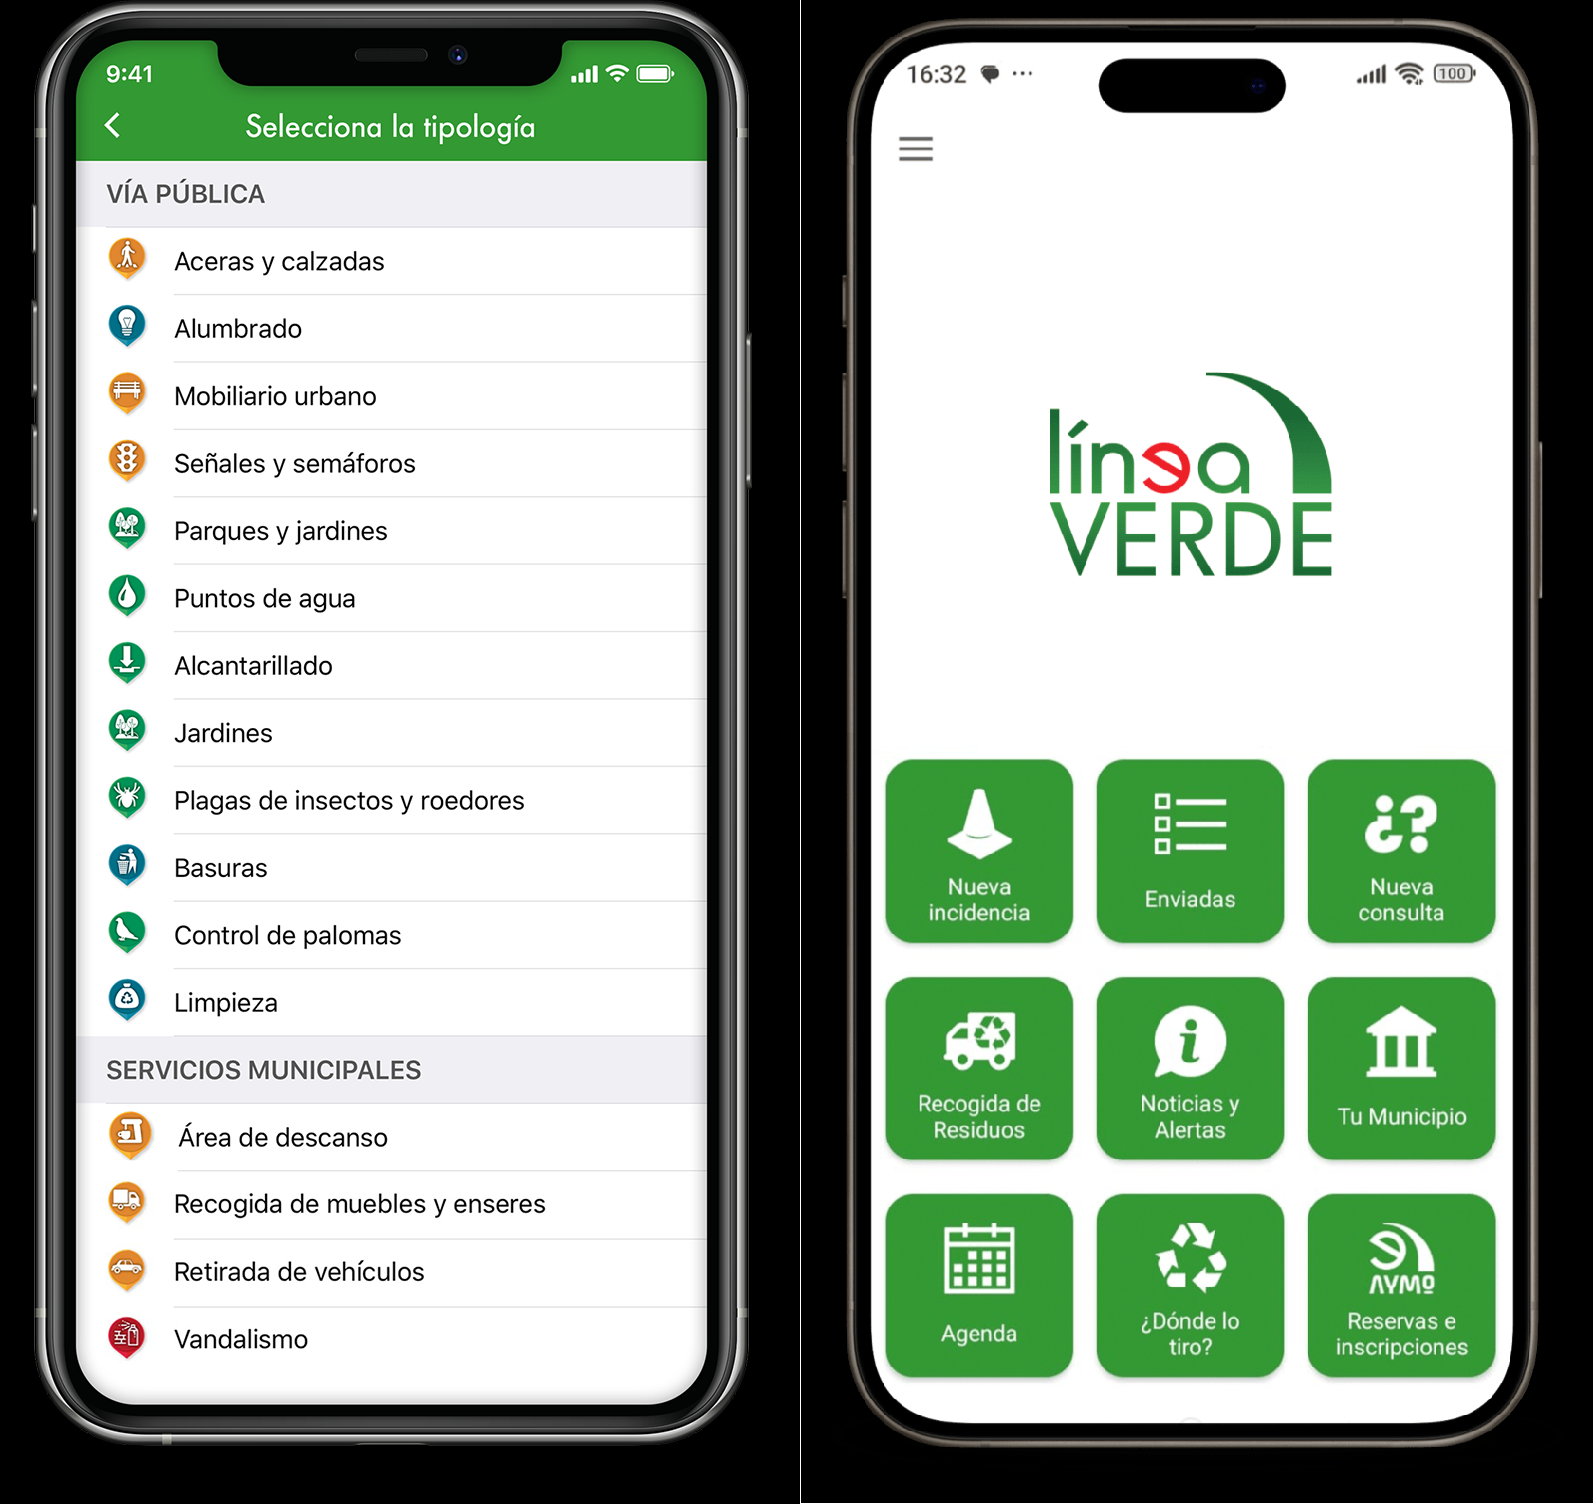
\includegraphics[width=0.7\textwidth]{imaxes/arte/linea_verde.png}
  \caption{Vista de la app Línea Verde}
  \label{fig:LíneaVerde}
\end{figure}

Línea Verde \cite{linea_verde} es una plataforma municipal de participación ciudadana y gestión de incidencias. Está bien orientada a comunicación con la administración, pero su foco es urbano y no operativo para emergencias.

\subsubsection{S.O.S Emergencias}

\begin{figure}[H]
  \centering
  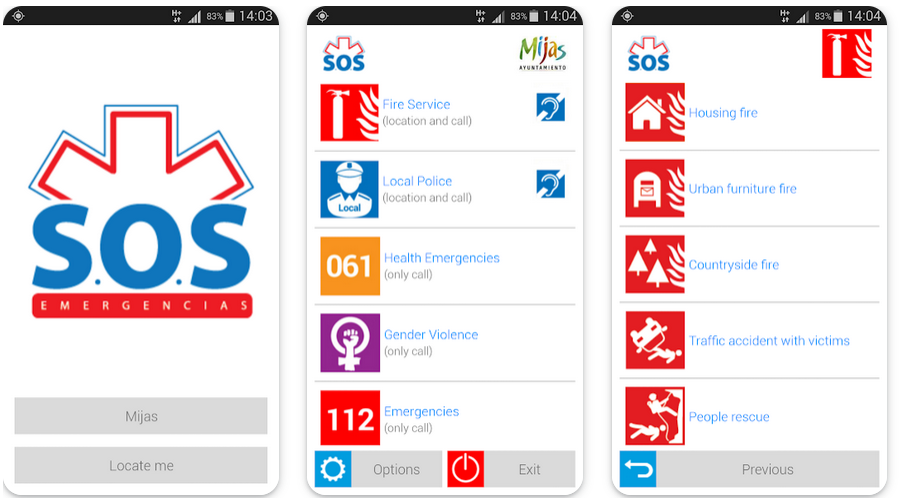
\includegraphics[width=0.7\textwidth]{imaxes/arte/sos_emergencias.png}
  \caption{Vista de la app S.O.S Emergencias}
  \label{fig:SOSEmergencias}
\end{figure}

S.O.S Emergencias \cite{sos_emergencias} es una aplicación móvil orientada a la notificación y gestión básica de emergencias. Aporta una aproximación más directa al ámbito de alertas, aunque no integra una visión completa de coordinación geoespacial y despliegue de recursos.

\section{Iniciativas públicas recientes}
\label{sec:arte-public}
En un comunicado, la Xunta de Galicia ha anunciado la ampliación de mecanismos de detección temprana de incendios forestales mediante la creación de una nueva app para la ciudadanía junto con el uso de cámaras de videovigilancia \cite{xunta_deteccion_incendios_2026}.

Esta aplicación combina un canal para notificaciones tempranas, sensores y cámaras para observación remota y procesamiento automatizado con IA para priorizar alertas y detectar anomalías. Todo ello ayuda a la notificación y coordinación de emergencias en tiempo real.

Funcionalmente esta nueva app parece converger mucho con el dominio funcional de la solución precedente \cite{TFGAdrianGarcia2025}: reportes ciudadanos, integración de sistemas de información dispares como avisos ciudadanos y meteorológicos y también cuenta con representación geoespacial; a efectos prácticos la solución de la Xunta incorpora muchas de las ideas que se prototiparon en el trabajo previo.

Algunas diferencias clave respecto a la solución inicial son que la aplicación añade una capa de hardware y vigilancia (cámaras/sensores) y está diseñada para integrarse en procedimientos administrativos y operativos a escala autonómica. Por otro lado, aquella primera propuesta aporta un énfasis en la coordinación táctica, como la asignación de recursos, la gestión por cuadrantes y el soporte a decisiones de despliegue en campo.

Como comentario crítico, cabe destacar la coincidencia temática que resalta la relevancia del problema abordado en la propuesta previa y demuestra que las soluciones planteadas tienen aplicación real. Ambas aproximaciones son complementarias y evidencian la necesidad de soluciones integrales que aborden todo el ciclo de gestión de emergencias, desde la detección hasta la coordinación en campo.

\section{Conclusión}
Las aplicaciones analizadas ofrecen soluciones parciales en las tres dimensiones de interés: gestión de avisos, representación geoespacial y coordinación de equipos. Ninguna de las herramientas revisadas integra de forma nativa las tres capacidades con enfoque ciudadano-operativo y despliegue de recursos; esto evidencia el hueco funcional que aborda la propuesta de este trabajo.

La tabla comparativa 3.1 resume las funcionalidades analizadas para resaltar fortalezas y carencias de cada alternativa:

\begin{table}[H]
  \centering
  \resizebox{\textwidth}{!}{
    \rowcolors{2}{white}{udcgray!25}
    \begin{tabular}{c|c|c|c|c|c|c|c|c}
      \rowcolor{udcpink!25}
      &
      \begin{tabular}[c]{@{}l@{}}Visualización \\ geográfica\end{tabular} &
      \begin{tabular}[c]{@{}l@{}}Datos \\ meteorológicos\end{tabular} &
      \begin{tabular}[c]{@{}l@{}}Gestión de \\ personal y recursos\end{tabular} &
      \begin{tabular}[c]{@{}l@{}}Plan gratuito \\ suficiente\end{tabular} &
      \begin{tabular}[c]{@{}l@{}}Plugins \\o margen de mejora\end{tabular} & 
      \begin{tabular}[c]{@{}l@{}}Sistema de avisos \\o notificaciones\end{tabular} &
      \begin{tabular}[c]{@{}l@{}}Multi-\\emergencia\end{tabular} &
      \begin{tabular}[c]{@{}l@{}}App \\ móvil\end{tabular} \\
      \textit{Jira} &  &  & \checkmark & \checkmark & \checkmark & \checkmark & \checkmark & \checkmark \\
      \textit{Asana} &  &  & \checkmark & \checkmark & \checkmark & \checkmark & \checkmark & \checkmark \\
      \textit{Línea Verde} & \checkmark &  & \checkmark & \checkmark & & \checkmark & \checkmark & \checkmark \\
      \textit{SOS Emergencias} & & & \checkmark & \checkmark & & \checkmark & \checkmark & \checkmark \\
      \textit{Global Forest Watch - Fires} & \checkmark & \checkmark &  & \checkmark &  & \checkmark &  &  \\
      \textit{InciWeb} & \checkmark &  &  & \checkmark &  &  &  &  \\
      \textit{Google Maps} & \checkmark &  &  & \checkmark & \checkmark &  &  & \checkmark \\
      \textit{Microsoft Teams} &  &  & \checkmark & \checkmark & \checkmark & \checkmark & \checkmark & \checkmark \\
      \textit{Odoo} &  &  & \checkmark & \checkmark & \checkmark & \checkmark & \checkmark & \checkmark \\
      \textit{PCAM Gestión} & \checkmark &  & \checkmark &  & \checkmark & \checkmark & \checkmark & \checkmark \\
      \textit{XeoCode Lite} & \checkmark & ? & \checkmark & ? & ? & ? & ? & ? \\
      \textit{Xunta (nueva app)} & \checkmark & \checkmark &  & \checkmark &  & \checkmark &  & \checkmark \\
    \end{tabular}}    
    \caption{Tabla comparativa entre aplicaciones}
    \label{tab:comparativa}
\end{table}

 \chapter{Análisis de viabilidad}
\label{chap:viabilidade}

\lettrine{E}{n este capítulo} se analiza la viabilidad del proyecto desde tres perspectivas complementarias: dimensión temporal, dimensión tecnológica y dimensión económica. 

\section{Viabilidad temporal}
Para la realización de este TFM se ha estimado una duración aproximada de cuatro meses. Dicha planificación incluye las fases de análisis, diseño, implementación, pruebas y redacción de la memoria. Además, se contempla la familiarización de las nuevas tecnologías. Dado el alcance definido la viabilidad temporal es aceptable y no representa un riesgo crítico para la finalización del proyecto.

La metodología usada utiliza desarrollos cortos para ir validando el progreso y ajustando el alcance si fuera necesario.

\section{Viabilidad tecnológica}
Para el estudio de viablidad tecnológica se han considerado las tecnologías heredadas del TFG, así como las nuevas tecnologías propuestas para el desarrollo de la aplicación móvil y la integración de notificaciones push.

En resumen, el stack tecnológico propuesto para el TFM es el siguiente:
\begin{itemize}
  \item Backend: Spring Boot (Java) para servicios REST y la integración con PostgreSQL/PostGIS.
  \item Base de datos: PostgreSQL con PostGIS para soporte espacial.
  \item Frontend web: React con Material-UI para interfaces ricas.
  \item Aplicación Android: Kotlin y Jetpack Compose para la capa de presentación; cliente nativo para acceder a sensores y recibir notificaciones push.
  \item Notificaciones push: Firebase Cloud Messaging (FCM) para la entrega fiable de mensajes a dispositivos Android.
\end{itemize}

Kotlin y FCM merecen una mención específica: ambas tecnologías están ampliamente adoptadas, cuentan con extensa documentación y comunidades activas, y existen guías oficiales para su integración con backends Java/Spring. Por tanto, su adopción no supone un riesgo tecnológico significativo; aportan ventajas en productividad, interoperabilidad móvil y soporte nativo para notificaciones.

Las demás tecnologías son conocidas por el autor gracias a su dedicación profesional y al proyecto previo, lo que reduce el riesgo de adopción y acelera el desarrollo.


\section{Viabilidad económica}
El proyecto no requiere una inversión económica significativa en hardware o licencias de software. El software utilizado es mayoritariamente Open Source (Spring Boot, PostgreSQL, React, Kotlin/Jetpack Compose), por lo que no hay costes de licencia en el entorno de desarrollo académico.

En el ámbito del desarrollo y las pruebas estos pueden ejecutarse con recursos disponibles por lo que no es necesario adquirir nuevo hardware.Sobre el uso de servicios en la nube o APIs de terceros(FMC, MapLibre, OpenWeatherMap) pueden surgir costes, pero se pueden controlar gracias a los planes gratuitos o a la monitorización de uso.

La dimensión económica no supone un riesgo significativo para la ejecución del TFM pues los costes directos son bajos.

\section{Conclusión del análisis de viabilidad}
En resumen, el proyecto es totalmente viable porque combina un plan de trabajo realista de cuatro meses con un uso inteligente de la tecnología. Al reutilizar la base del TFG y apoyarse en herramientas gratuitas y potentes como Kotlin y FCM, el riesgo técnico es mínimo y el coste es prácticamente cero. Esta experiencia previa, sumada a una planificación clara, garantiza que el proyecto se pueda terminar a tiempo y con la calidad necesaria para un TFM.


 \chapter{Introducción al desarrollo realizado}
\label{chap:desenrolo}

\section{Introducción}


\lettrine{E}{n} este capítulo se presenta una descripción del desarrollo realizado, los objetivos perseguidos y la metodología aplicada durante la implementación. El propósito es ofrecer un vistazo general de los artefactos construidos y de las decisiones más relevantes tomadas durante el desarrollo del proyecto.

\section{Arquitectura de la Solución}


\vspace{1em}

{ \color{red} PENDIENTE una vez avanzado más el proyecto }

\section{Metodología e iteraciones}

El proceso de desarrollo se organizó mediante iteraciones cortas con objetivos funcionales concretos, siguiendo las ideas de Scrum adaptadas al contexto de trabajo individual. Aunque no se aplicó una implementación completa y formal de Scrum (debido al tamaño reducido del equipo), se adoptaron sus pilares fundamentales: planificación por sprints, revisiónes y \emph{feedback} contínuo.

En cuanto a roles, el autor del \acrshort{tfm} asumió las responsabilidades de desarrollo y encargado de definición funcional, mientras que el tutor actuó como responsable de supervisión y de aceptación.

Se establecieron reuniones de revisión mensuales con el tutor en las que se presentaron los artefactos construidos (prototipos, endpoints, pantallas, pruebas y documentación). Estas sesiones sirvieron para validar funcionalidades, priorizar tareas y ajustar el dominio del \acrshort{tfm} y el alcance de las siguientes iteraciones.

El proyecto se estructuró en una serie de sprints. De una forma resumida, las fases necesarias para realizar este \acrshort{tfm} fueron: una fase inicial de contextualización y definición del valor del proyecto; la creación del esqueleto y la arquitectura base de la aplicación móvil para facilitar el desarrollo posterior; la normalización y actualización del modelo de recursos y organizaciones manteniendo compatibilidad con las entidades Equipo y Vehículo; la implementación de la gestión de emergencias y asignaciones básicas; la introducción de un esquema de logs operativos y la migración o compatibilidad con tablas legacy; la integración de notificaciones móviles mediante \acrshort{fcm} y el flujo de aceptación de asignaciones; y, finalmente, la implementación de capacidades semiautomáticas junto a un motor de reglas sencillo para generar propuestas automáticamente.

Para la planificación y el detalle de cada sprint se describen con mayor extensión en el capítulo de planificación (capítulo \ref{sec:sprints}).

 \chapter{Planificación y análisis de costes}
\label{chap:planificacionycostes}

\lettrine{E}{n} este capítulo se presenta la planificación aplicada durante el desarrollo del proyecto y un análisis de los costes asociados. Se describe la planificación inicial, las sprints que han estructurado el trabajo y las desviaciones observadas en el seguimiento.

\section{Planificación}
\label{sec:planificacion}

La planificación inicial se definió en 9 sprints, cada una organizada internamente siguiendo el modelo clásico de cuatro fases: análisis, diseño, implementación y pruebas. La estimación de esfuerzo inicial se basó en jornadas de 6 horas diarias y en una duración prevista del proyecto de cuatro meses. No obstante, las complejidades técnicas y errores imprevistos motivaron desviaciones en varias iteraciones, tal y como se comenta en la sección de seguimiento.

\begin{table}[H]
  \centering
  \resizebox{\textwidth}{!}{
    \rowcolors{2}{white}{udcgray!25}
    \begin{tabular}{l|c|c|c}
      \rowcolor{udcpink!25}
      \textbf{Tarea} & \textbf{Fecha inicio} & \textbf{Días estimados} & \textbf{Días reales} \\

      Definición tipos Emergency & 04/03 & 0.5 & 0.5 \\
      Definición modelo Assignment & 04/03 & 0.5 & 0.5 \\
      Definición contratos OpenApi & 04/03 & 1 & 1 \\
      Diseño entidades JPA & 05/03 & 0.5 & 0.5 \\

      Implementación entidad Emergency & 06/03 & 0.5 & 0.5 \\
      Implementación entidad Assignment & 06/03 & 0.5 & 0.5 \\
      Implementación repositorios & 06/03 & 0.5 & 0.5 \\

      UseCase Emergency & 08/03 & 0.5 & 0.5 \\
      UseCase Assignment & 08/03 & 0.5 & 0.5 \\

      Endpoints /emergencies & 09/03 & 0.5 & 0.5 \\
      Endpoints /assignments & 09/03 & 0.5 & 0.5 \\

      Tests unitarios backend & 11/03 & 1 & 1 \\
      Tests integración backend & 11/03 & 1 & 1 \\

      Consumir Api desde frontend & 10/03 & 0.5 & 0.5 \\
      Vista mapa (crear Emergency) & 11/03 & 1 & 1 \\
      Formulario Emergency & 11/03 & 0.5 & 0.5 \\
      Listado Emergencies & 12/03 & 0.5 & 0.5 \\
      Actualización UI Assignment & 12/03 & 1 & 1 \\
      Listado Assignments & 13/03 & 0.5 & 0.5 \\

      Consumir Api desde Android & 07/03 & 0.5 & 0.5 \\
      Lista Assignments Android & 12/03 & 1 & 1 \\
      Detalle Assignment Android & 13/03 & 0.5 & 0.5 \\
      Corrección bugs & 15/03 & 1 & 1 \\

    \end{tabular}
  }
  \caption{Planificación del Sprint 3: Emergencias y asignaciones básicas}
  \label{tab:sprint3}
\end{table}

En la tabla~\ref{tab:sprint3} se puede observar un desglose del sprint 3, que se centró en la implementación de la gestión de emergencias y asignaciones básicas. Cada tarea se estimó inicialmente en función de su complejidad, esto sirvió para poder observar desviaciones y ajustar la planificación de los siguientes sprints. En este caso, el sprint se completó dentro del plazo previsto, lo que permitió mantener el ritmo de desarrollo planificado.


\section{Sprints}
\label{sec:sprints}

El proyecto se estructuró en una sucesión de sprints, cada uno de los cuales incrementaba la funcionalidad de los artefactos entregados.  A continuación se detalla cada sprint con sus objetivos y resultados principales.

\subsection{Sprint 0: Contextualización}
En esta fase inicial se realizó la contextualización del dominio y la justificación del valor del \acrshort{tfm}. Se investigaron fuentes, alternativas a la aplicación y tecnologías potenciales (mapas, sistema de notificaciones android, sistema de recomendación y reglas básico). El objetivo fue delimitar el alcance y dominio del proyecto para que este sea viable en un espacio temporal acotado.

\subsection{Sprint 1: Esqueleto y arquitectura base de aplicación móvil}
Se creó el esqueleto del proyecto móvil y se definieron las dependencias y la arquitectura base (estructura de paquetes, patrones de navegación, y la configuración inicial de Jetpack Compose). Además se implementaron los módulos iniciales de autenticación y sincronización con el Backend (endpoints básicos) para poder iterar sobre funcionalidades reales.

\subsection{Sprint 2: Actualizar la organización de recursos}
Se introdujo el modelo unificado de recursos y organizaciones preservando la compatibilidad con las entidades Legacy (Equipo y Vehículo). Esto incluyó definir atributos de capacidad, áreas operativas (cuadrantes) y las relaciones necesarias a nivel de base de datos y DTOs. Se arreglaron los endpoints antiguos y DTO's parara la gestión CRUD de organizaciones y sus recursos.

\subsection{Sprint 3: Emergencias y asignaciones básicas}
Se implementó la gestión de emergencias con soporte para dos tipos de localización: punto y cuadrante. Se añadió la creación y edición de Emergencias, la definición de cuadrantes y una primera versión del flujo de creación de Asignaciones. Esta iteración incluyó validaciones de consistencia (ej. comprobar que un cuadrante pertenece a una emergencia) y pruebas de integración explicitas para el servicio de Asignaciones.

\subsection{Sprint 4: Nuevo sistema de logs operativos}

Se definió un nuevo esquema para los logs operativos, ahora centralizados en las Asignaciones de recursos en las emergencias. El trabajo abarcó el nuevo modelado y la persistencia que permiten conservar el histórico.

\subsection{Sprint 5: Notificaciones en Android y aceptación de asignaciones}
Se integró Firebase Cloud Messaging (\acrshort{fcm}) en la aplicación Android: registro de MobileDevice, manejo de tokens y recepción de notificaciones. Se implementó el flujo de envío de notificaciones desde el Backend y la experiencia de usuario en la app para aceptar o rechazar asignaciones recibidas.

\subsection{Sprint 6: Protocolos semiautomáticos (motor de reglas simple)}
Se introdujo la capacidad de definir Protocols almacenados en \acrshort{jsonb} y un motor de reglas ligero que permite generar propuestas de Asignaciones de forma semiautomática en el frontend. Esto incluyó la definición del formato JSON para los protocolos, la implementación de un evaluador simple y la integración con el pipeline de creación de propuestas.

\subsection{Sprint 7 y 8: Finalización, pruebas y despliegue}
Las iteraciones finales se dedicaron a la estabilización: pruebas end-to-end, ajuste de UX tanto del frontal como de la aplicación Android, corrección de errores, poblamiento de datos de ejemplo y preparación de artefactos de despliegue (contenedores Docker para BBDD y servicio). También incluyeron la redacción y revisión de la memoria y la generación de la documentación.

\section{Seguimiento}
\label{sec:seguimiento}

El seguimiento se llevó a cabo mediante reuniones mensuales con el tutor y el uso de un tablero Kanban de tareas que permitía visualizar el estado de ellas. En cada revisión se presentaron artefactos funcionales (pantallas, endpoints, wireframes).

Las desviaciones más relevantes provinieron de problemas técnicos con la representación de cuadrantes en el mapa, configuración de la aplicación Android y el motor de reglas básico para los protocolos. 

\section{Análisis de costes}
\label{sec:costes}

El análisis de costes se ha planteado distinguiendo entre costes directos de personal, costes indirectos de infraestructura y un margen de contingencia para imprevistos. Para la valoración económica del esfuerzo se han tomado como referencia salarios publicados por Talent.com para España, donde un perfil de \textit{Programador} se sitúa en 27.500~\euro/año (14,10~\euro/h)  \cite{salario_programador}y un perfil de \textit{Analista programador} en 29.120~\euro/año (14,93~\euro/h)~\cite{salario_analista_programador}. Estos valores resultan razonables para un TFM técnico con tareas de análisis, desarrollo, pruebas e integración.

\subsection{Estimación del esfuerzo}

La planificación se ha estructurado en 7 sprints. Si se asume una duración media de 2 semanas por sprint, el proyecto cubre aproximadamente 14 semanas de trabajo efectivo. Considerando una dedicación máxima de 6 horas al día y trabajo únicamente de lunes a viernes, el esfuerzo total estimado se calcula como sigue:

\[
7\ \text{sprints} \times 2\ \text{semanas/sprint} \times 5\ \text{días/semana} \times 6\ \text{h/día} = 420\ \text{horas}
\]

Este valor representa una estimación prudente del esfuerzo total del proyecto. La distribución del tiempo no es homogénea entre sprints, ya que las primeras iteraciones requieren más análisis y diseño, mientras que las finales concentran más trabajo de integración, pruebas, corrección de errores y documentación.

\subsection{Costes directos de personal}

Para la valoración del trabajo se ha tomado como base el perfil de \textit{Analista programador}, al ser el que mejor refleja un proyecto de estas características, donde una misma persona asume tareas de definición funcional, implementación y validación. Con la tarifa media indicada por la fuente utilizada, el coste directo estimado es:

\[
420\ \text{h} \times 14,93\ \text{\euro/h} = 6.270,60\ \text{\euro}
\]

De forma complementaria, si se valorase el trabajo con el perfil de \textit{Programador}, el coste sería:

\[
420\ \text{h} \times 14,10\ \text{\euro/h} = 5.922,00\ \text{\euro}
\]

Para reflejar ambas referencias, se adopta como coste base del proyecto el punto medio entre ambos perfiles, es decir, \textbf{6.096,30~\euro}, que representa mejor la mezcla de tareas de programación y análisis realizada durante el desarrollo.

\subsection{Costes indirectos}

A los costes de personal se añaden los costes indirectos de ejecución. Para este tipo de proyecto, los más relevantes son la amortización del equipo de trabajo y los suministros básicos asociados al desarrollo:

\begin{itemize}
  \item Amortización de hardware: se considera el uso de un equipo portátil de desarrollo valorado en 900~\euro, con una vida útil de 4 años. Para un proyecto de unos 3,5 meses, el coste imputable es de aproximadamente 66,00~\euro.
  \item Conectividad y suministros: se estiman 40~\euro/mes de internet y 30~\euro/mes de electricidad proporcional al tiempo de desarrollo. Para 3,5 meses, esto supone 245,00~\euro.
\end{itemize}

\subsection{Resumen económico}

\begin{table}[H]
  \centering
  \rowcolors{2}{white}{udcgray!25}
  \resizebox{1\textwidth}{!}{%
    \begin{tabular}{c|c|c|c|c}
      \rowcolor{udcpink!25}
    Concepto & Importe estimado (\euro) & Observaciones \\
    Coste directo de personal & 6.096,30 & Media entre programador y analista programador \\
    Amortización de hardware & 66,00 & Portátil de desarrollo imputado al proyecto \\
    Conectividad y suministros & 245,00 & Internet y electricidad proporcionales \\
    \hline
    \textbf{Total estimado} & \textbf{6.407,3} & \\
    \hline
   \end{tabular}%
  }
  \caption{Desglose de costes estimados del proyecto}
  \label{tab:costes_resumen}
\end{table}

La tabla~\ref{tab:costes_resumen} muestra que el mayor peso del presupuesto corresponde al trabajo humano, seguido por los costes de infraestructura y suministros. Esto es coherente con un proyecto de software de ámbito académico, donde la inversión principal no está en equipamiento especializado sino en la dedicación de horas de desarrollo, integración y validación.


\subsection{Conclusión del análisis de costes}

El coste final del proyecto asciende a \textbf{6.407,3\euro} con una dedicación total de \textbf{420 horas}. Estas cifras reflejan el alcance y la coste del \acrshort{tfm}, considerando tanto el esfuerzo humano como los recursos materiales necesarios para su ejecución. Es importante destacar que esta estimación se ha realizado con criterios prudentes y basándose en datos salariales reales, lo que aporta una visión más ajustada del valor económico del trabajo realizado en este proyecto.

 \chapter{Requisitos del sistema}
\label{chap:requisitos}

\lettrine{E}{n} este capítulo se describen los requisitos funcionales y los actores principales del sistema. La solución evoluciona respecto al \acrshort{tfg} ampliando el alcance desde la coordinación centrada en incendios forestales hacia una plataforma multi-riesgo, con un flujo más completo de aviso, validación, creación de emergencias y asignación de recursos.

\section{Introducción}

Los tres pilares funcionales de la aplicación siguen siendo la gestión de avisos, la gestión de emergencias y la gestión de personal y recursos, pero en este \acrshort{tfm} se redefinen para cubrir un dominio más amplio. Los usuarios no autenticados o ciudadanos pueden registrar avisos sobre emergencias con sus imágenes adjuntas y consultar posteriormente el estado de dichos avisos.

Sobre esos avisos actúa un administrador o coordinador, que revisa la información recibida y decide si procede crear una emergencia. A diferencia del \acrshort{tfg}, donde el foco estaba más ligado al incendio forestal y a una organización más estática de equipos, en este trabajo la emergencia puede vincularse a unas coordenadas en concreto, cuando el incidente está localizado con precisión, o como una colección de cuadrantes, cuando este afecta a una zona más amplia. 

Una vez creada la emergencia, el administrador puede seguir los protocolos estipulados y realizar una asignación manual de los recursos, pero ahora el sistema ofrece una propuesta de asignación de recursos a dicho coordinador. Este mecanismo filtra candidatos en función de la organización a la que pertenecen, de su estado operativo y de su distancia a la emergencia. 

El flujo operativo se completa con el envío de notificaciones a los usuarios de los equipos asignados, de forma que el jefe de equipo pueda aceptar la emergencia y se actualice el estado del recurso a ocupado o desplegado. En el caso de los vehículos, la aceptación se resuelve de forma automática. Finalmente, cuando la emergencia se completa, el recurso pasa de nuevo a estado disponible.

La principal ampliación funcional respecto al \acrshort{tfg} es la introducción de un rol adicional de miembro de equipo. Así, el sistema distingue ahora entre ciudadano, miembro de equipo, manager y coordinador. El ciudadano conserva un perfil muy reducido, centrado en crear avisos y consultar el estado de sus notificaciones. El miembro de equipo accede al seguimiento de sus asignaciones, el manager mantiene funciones de organización y gestión operativa, y el coordinador conserva las capacidades de validación, creación de emergencias y supervisión global del sistema.

\section{Actores}

En el contexto de una plataforma de coordinación de emergencias, resulta fundamental definir con claridad los actores que interactúan con el sistema. Cada actor representa un perfil de usuario con un conjunto concreto de capacidades, un nivel de acceso determinado y unas responsabilidades asociadas a la gestión de avisos, emergencias, recursos y asignaciones.

En este proyecto se han identificado los siguientes actores:

\begin{itemize}
    \item \textbf{Usuario no autenticado (ACT01)}: puede consultar el mapa general y crear un aviso de emergencia sin necesidad de iniciar sesión.
    \item \textbf{Usuario registrado (ACT02)}: además de las funciones básicas, puede consultar sus propios avisos y acceder al mapa y a las notificaciones personales.
    \item \textbf{Miembro de equipo (ACT03)}: dispone de acceso a la información operativa de su equipo, a las emergencias activas y a las asignaciones asociadas.
    \item \textbf{Responsable de equipo o gestor de recursos (ACT04)}: puede gestionar equipos y vehículos, asignar y retirar recursos, y operar sobre emergencias activas dentro de su ámbito de responsabilidad.
    \item \textbf{Coordinador (ACT05)}: asume el mayor nivel de permisos y gestiona usuarios, organizaciones, avisos, emergencias, asignaciones y reglas de recomendación.
\end{itemize}

\begin{figure}[H]
  \centering
  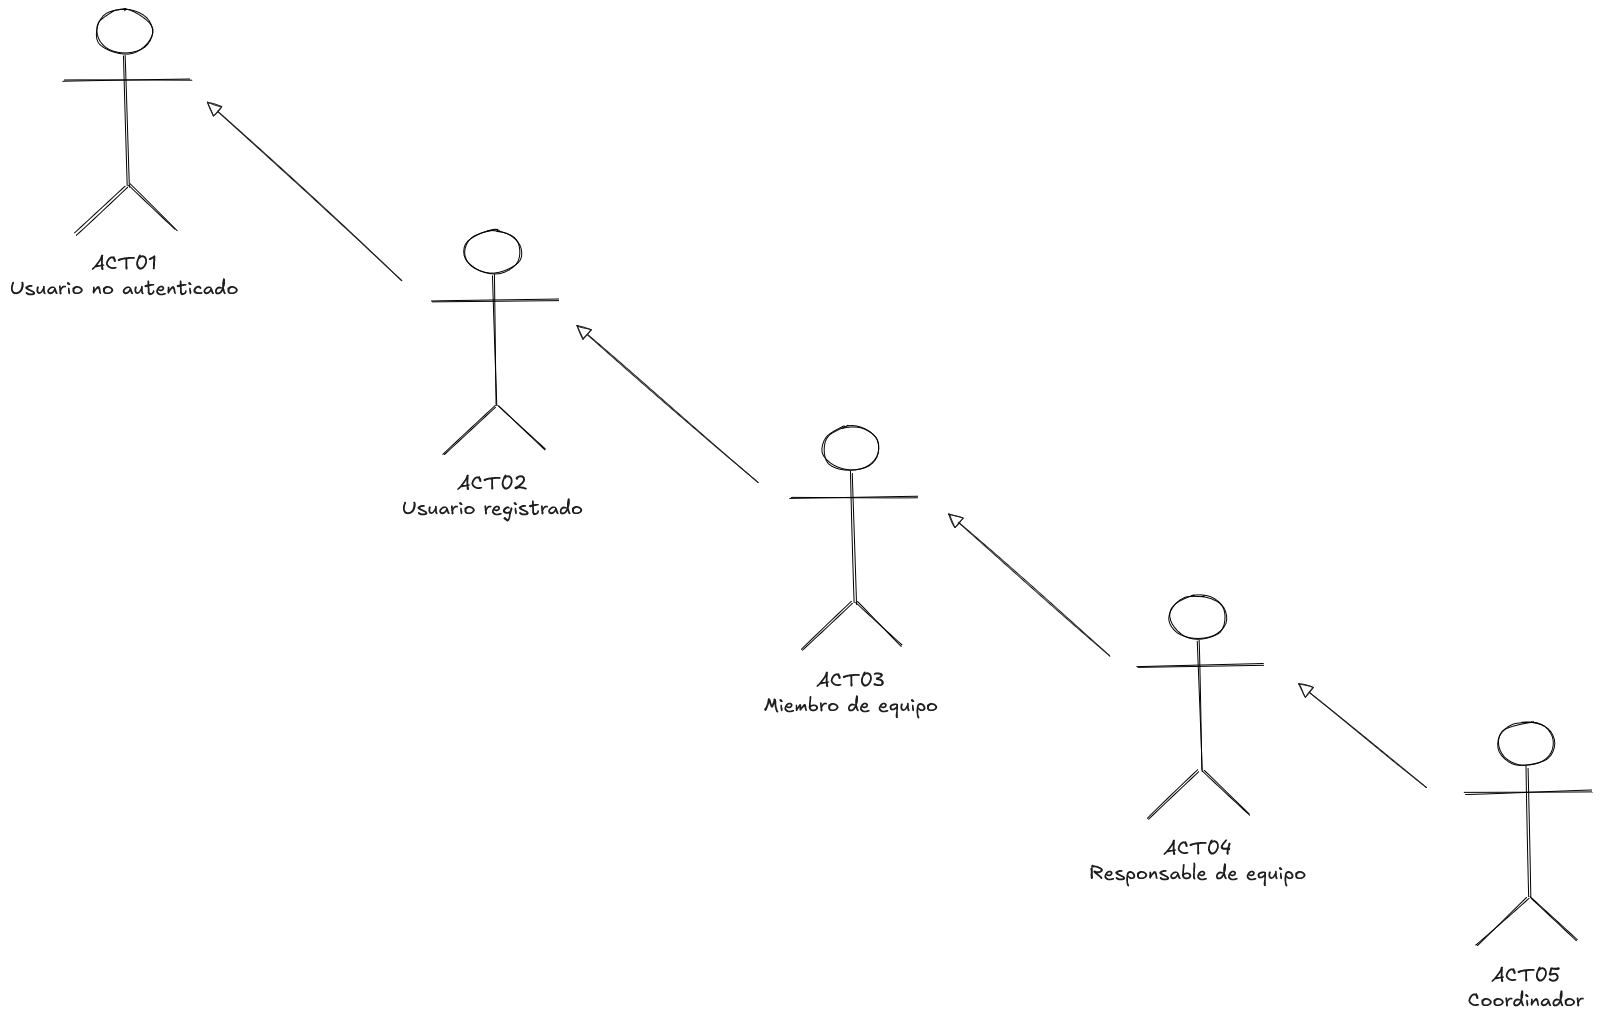
\includegraphics[width=1\textwidth]{imaxes/diagrama-actores.png}
  \caption{Diagrama de la jerarquía de actores del sistema}
  \label{fig:actores-sistema}
\end{figure}

Además, los permisos siguen una jerarquía acumulativa, como se muestra en la figura \ref{fig:actores-sistema}. Esto significa que cada actor superior hereda las capacidades del nivel anterior y añade nuevas funcionalidades. De este modo, el usuario no autenticado posee las capacidades más limitadas, entre ellas se encuentra la visualización del mapa de emergencias y la creación de avisos, mientras que el coordinador, a mayores de las funcionalidades de los roles anteriores cuenta con la capacidad de gestionar usuarios, organizaciones, emergencias y asignaciones, así como de configurar las reglas de recomendación para la asignación automática de recursos. Esta estructura jerárquica facilita la gestión de permisos y asegura que cada usuario tenga acceso únicamente a las funciones necesarias para su rol específico dentro del sistema.

\section{Casos de uso}

{ \color{red} Aspectos a considerar
    \begin{itemize}
      \item Agrupar casos de uso (servirá de base para agruparlos en servicios posteriormente en la sección de diseño).
      \item Definición concreta /detallada de cada caso de uso (precondiciones ...)
    \end{itemize}
}

\section{Modelo de casos de uso}

{ \color{red} Aspectos a considerar
    \begin{itemize}
      \item Diagrama de casos de uso incluyendo actores y relaciones entre casos
    \end{itemize}
}

\section{Prototipado de interfaz}

{ \color{red} Es interesante hacer el esfuerzo en este momento de prototipar las principales pantallas de la interfaz (y añadirlas en la memoria), como parte del análisis de requisitos, así como de aspectos de usabilidad de las mismas. }

 \chapter{Diseño}
\label{chap:deseño}

\lettrine{E}{n} este capítulo se describe la organización interna de la aplicación y las principales decisiones de diseño adoptadas en sus tres subsistemas: backend, frontend y Android. El objetivo ha sido mantener una estructura coherente con el dominio funcional del proyecto, facilitar el mantenimiento del código y conservar una separación clara entre persistencia, lógica de negocio, exposición de servicios e interfaz de usuario.

\section{Introducción y objetivos}

El diseño parte de una idea principal: el sistema debe permitir coordinar emergencias, recursos y avisos de forma consistente, sin duplicar responsabilidades entre capas. Para ello, el backend concentra el modelo de dominio y las reglas de negocio, el frontend web actúa como interfaz de gestión principal y la aplicación Android adapta parte de esas funcionalidades a un contexto móvil, manteniendo el acceso a la información operativa y a las acciones más frecuentes.

En la evolución respecto al trabajo previo \cite{TFGAdrianGarcia2025} se han incorporado nuevas funcionalidades, especialmente en torno a las asignaciones, el envío de notificaciones y la generación de recomendaciones basadas en reglas. La estructura general de la interfaz y del dominio se mantiene porque el objetivo no era redefinir la aplicación completa sino ampliar su alcance funcional sobre una base ya establecida. Al existir una base escalable, se han podido añadir funcionalidades sin reestructurar completamente el sistema, si bien se han tenido que realizar modificaciones, aunque de menor complejidad de la que habría supuesto partir de un diseño completamente nuevo. 

\section{Resumen de patrones usados}
\label{sec:patrones}
Parte de la arquitectura y de las decisiones de diseño utilizadas en este proyecto han sido heredadas y adaptadas a partir del trabajo previo desarrollado. Esta reutilización no solo permite mantener una continuidad tecnológica, sino también reducir la complejidad de desarrollo al apoyarse en una base arquitectónica ya consolidada.

Entre los patrones heredados destaca especialmente la organización en capas, utilizada tanto en el backend como en el frontend, permitiendo separar claramente las responsabilidades de presentación, lógica de negocio y persistencia de datos. Esta división facilita el mantenimiento del código, mejora la modularidad y simplifica la evolución futura de la aplicación. Del mismo modo, se mantiene una estructura basada en el patrón Modelo-Vista-Controlador (MVC), especialmente en la parte de interfaz, favoreciendo una separación clara entre la representación visual, la gestión del estado y la interacción con el usuario.

También se utilizan mecanismos de abstracción y desacoplamiento como la inyección de dependencias, que facilita la reutilización de componentes y reduce el acoplamiento entre módulos, o el uso de objetos específicos para la transferencia de información entre capas, permitiendo encapsular y estructurar adecuadamente los datos intercambiados dentro del sistema. Además, se conservan patrones orientados al acceso y manipulación de datos, contribuyendo a aislar la lógica de persistencia del resto de la aplicación y mejorando la mantenibilidad general del proyecto.

Junto a estos patrones heredados, se han incorporado otros vinculados a la lógica de recomendación del backend y a la comunicación asíncrona y navegación de la aplicación Android. A continuación se resumen los principales patrones añadidos.

\begin{itemize}

    \item \textbf{API-first con OpenAPI:} En este proyecto se ha adoptado un diseño \textit{API-first}, definiendo primero el contrato de la API en un fichero YAML con OpenAPI y generando a partir de él las interfaces de controladores y los DTOs del backend mediante el plugin de Maven de OpenAPI. Gracias a esto se ha generado la documentación mediante Swagger de forma automática, lo que facilita la sincronización entre la implementación y la documentación y reduce errores de desalineación entre ambos. Este enfoque ha permitido que los contratos de la API se generen de forma consistente, lo que ha sido especialmente útil para integrar nuevas funcionalidades sin necesidad de modificar manualmente los contratos de datos.

    \item \textbf{Chain of Responsibility:} En el backend, la lógica de recomendaciones se apoya en este patrón, ya que las reglas se evalúan de forma secuencial hasta encontrar la primera que cumple la condición buscada. Cada regla actúa como un eslabón de la cadena y, cuando satisface el criterio, devuelve la propuesta asociada sin continuar con las siguientes.

    \item \textbf{Observer:} Este patrón aparece en varios puntos del proyecto. En Android, la integración con \textit{Firebase Messaging} se ajusta a este patrón, porque el dispositivo se suscribe mediante su token FCM y recibe notificaciones cuando el backend emite eventos relevantes. En el frontend, Redux sigue el mismo principio: los componentes se suscriben al store y se actualizan automáticamente cuando el estado global cambia, sin que el emisor de la acción tenga que conocer los suscriptores. Esta comunicación por eventos permite desacoplar el emisor del receptor en ambos entornos.

    \item \textbf{Fachada (Facade):} Este patrón se emplea en el backend para proporcionar una interfaz unificada que orquesta operaciones de alto nivel, delegando en servicios especializados y ocultando la complejidad subyacente a los controladores REST. De esta forma se simplifica la interfaz de la capa de lógica de negocio y se mantiene un acoplamiento bajo entre los controladores y los servicios de dominio.

    \item \textbf{Jetpack Compose:} En la parte Android se ha adoptado este enfoque declarativo para la interfaz, junto con una navegación por destinos mediante \textit{NavHost}. La aplicación sigue además un diseño de cliente ligero, apoyándose en el backend para la lógica de negocio y reservando para el móvil la composición de pantallas, la navegación y la interacción con el usuario.

\end{itemize}

\section{Arquitectura general}

La aplicación se organiza como un sistema cliente-servidor con tres subsistemas diferenciados. El backend implementa la lógica central del dominio y expone una \acrshort{api} \acrshort{rest}, el frontend web consume esa \acrshort{api} como una aplicación \acrshort{spa} y Android actúa como cliente móvil independiente que reutiliza el mismo backend.

Esta división permite que cada subsistema evolucione con una responsabilidad clara. El backend no depende de la tecnología de interfaz, el frontend web no contiene reglas de negocio relevantes y la aplicación Android adapta el consumo de datos a su navegación y a sus pantallas móviles.

El modelado utilizado en esta memoria sigue una perspectiva C4 \cite{C4Model}, comenzando por una vista de contexto que sitúa el sistema en su entorno y continuando con vistas de contenedor para cada uno de los subsistemas principales. 

\begin{figure}[H]
  \centering
  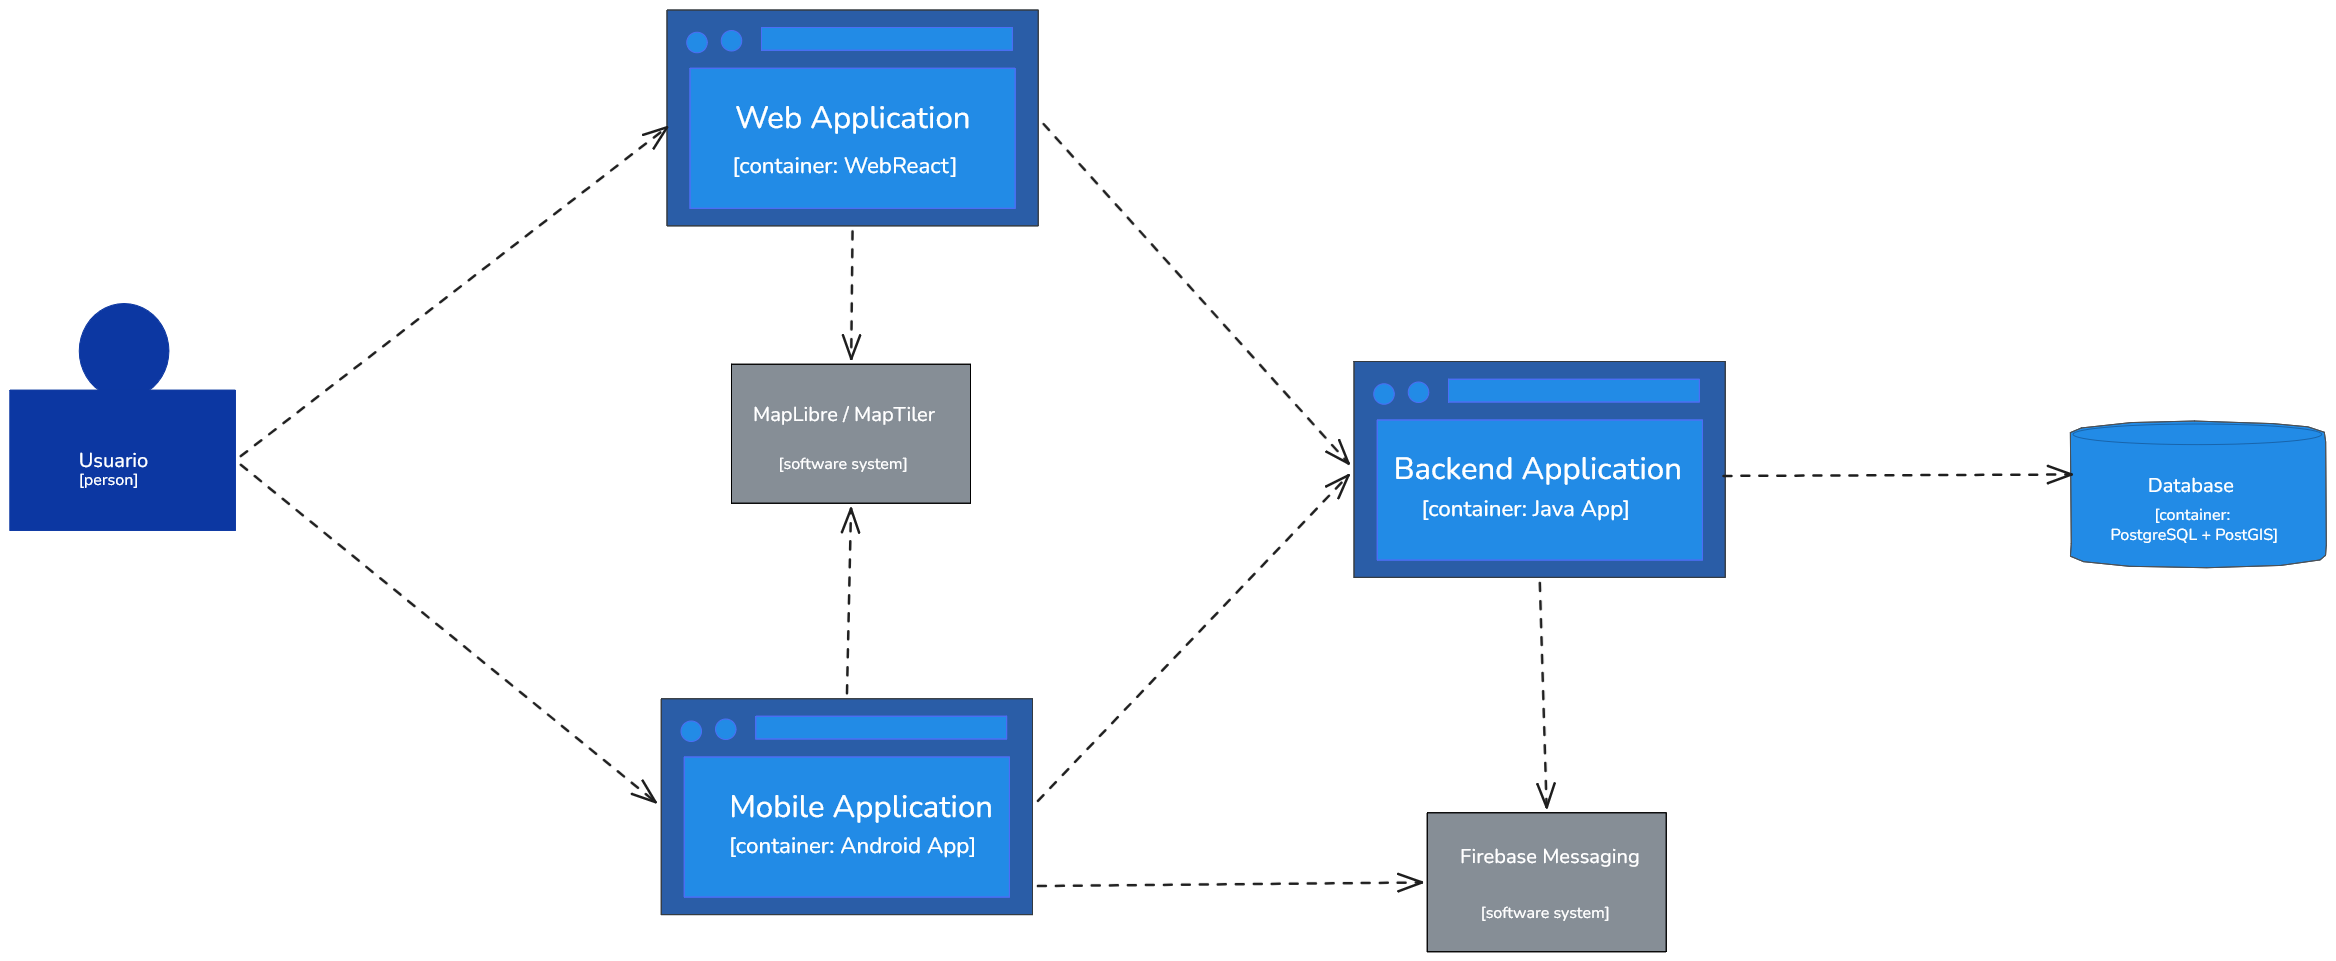
\includegraphics[width=\textwidth]{imaxes/c4/c4_contextual.png}
  \caption{Diagrama C4 de contexto de la aplicación}
  \label{fig:c4-contextual}
\end{figure}

En la figura \ref{fig:c4-contextual} se muestra la relación general entre los usuarios y los distintos sistemas con los que interactúa la aplicación. En esta vista de contexto se aprecia que el sistema central es el backend, que expone una \acrshort{api} \acrshort{rest} consumida tanto por el frontend web como por la aplicación Android. Además, el backend se integra con servicios externos como \acrshort{fcm} para notificaciones push y con una base de datos PostGIS para persistencia geoespacial. Los usuarios interactúan principalmente con el frontend web para gestión y consulta, mientras que la aplicación Android ofrece acceso móvil a información operativa y acciones frecuentes.

%%%%%%%%%%%%%%%%%%%%%%%%%%%%%%%%%%%%%%%%
% Subsistema Backend %
%%%%%%%%%%%%%%%%%%%%%%%%%%%%%%%%%%%%%%%%
\newpage
\section{Subsistema Backend}

\subsection{Objetivos}

El backend tiene como objetivo coordinar el estado de las emergencias, recursos, asignaciones y avisos. Debe exponer una \acrshort{api} \acrshort{rest} que permita al frontend web y a la aplicación Android consultar información operativa, gestionar emergencias, crear asignaciones, enviar avisos y configurar reglas de recomendación. Además, el backend debe garantizar la seguridad mediante autenticación y autorización, así como registrar históricos de las operaciones relevantes para trazabilidad y auditoría.

\subsection{Arquitectura}

La estructura del backend sigue un esquema clásico de Spring Boot. En la capa de entrada se encuentran los controladores \textit{REST}, que reciben las peticiones HTTP y devuelven \textit{DTOs}, que se transforman a representación JSON para ser devueltos. En la capa intermedia se sitúan las fachadas y servicios, donde se implementa la lógica de negocio. En la capa inferior están las entidades JPA y los repositorios, responsables de la persistencia.

\begin{figure}[H]
  \centering
  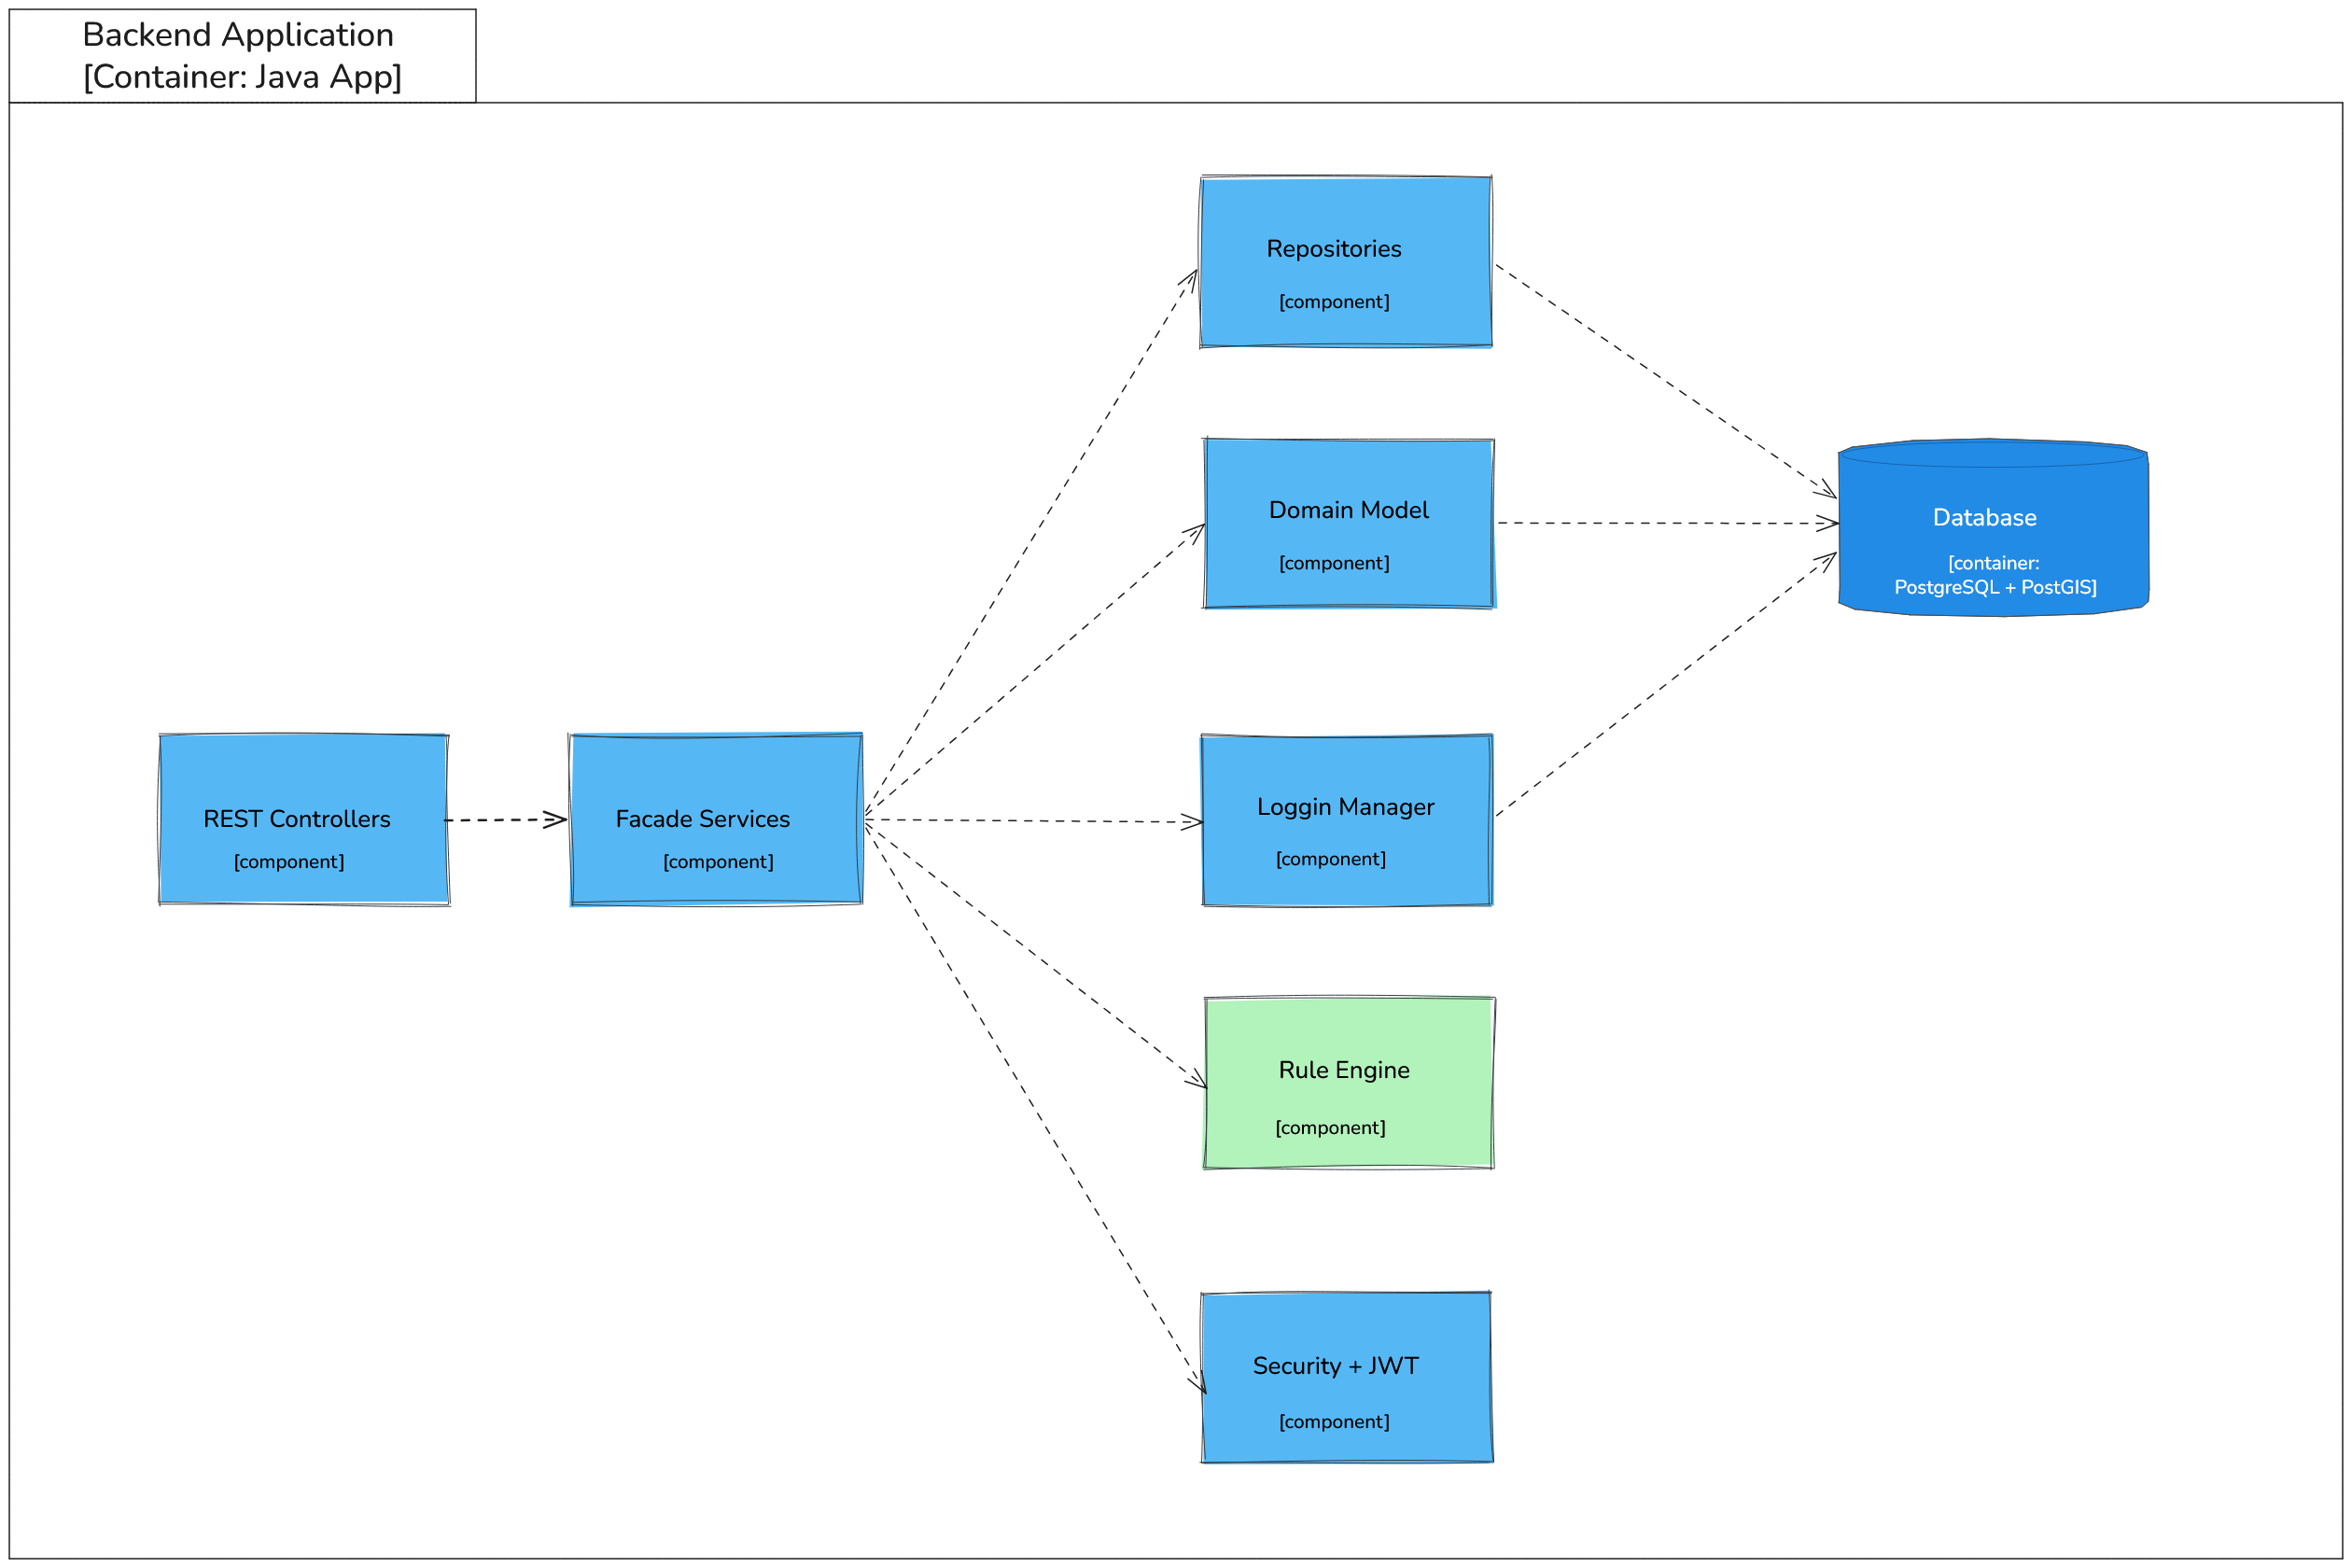
\includegraphics[width=0.7\textwidth]{imaxes/c4/c4_container_backend.png}
  \caption{Diagrama C4 de contenedores del backend}
  \label{fig:c4-container-backend}
\end{figure}

En la figura \ref{fig:c4-container-backend} se aprecia el contenedor backend y su descomposición en controladores, servicios fachada, modelo de dominio, repositorios, seguridad y gestión de históricos. La vista resume la estructura interna sin entrar en componentes más finos. 

Se ha utilizado el color verde para los nuevos componentes añadidos respecto al trabajo previo: la gestión de registros y el motor de reglas de recomendación. Los componentes existentes se han ampliado para dar soporte a las nuevas funcionalidades, como la gestión de asignaciones y la vinculación de emergencias a cuadrantes. Por ejemplo, el componente de dominio se ha extendido con nuevas entidades y relaciones, mientras que las fachadas han incorporado operaciones para gestionar asignaciones y reglas de recomendación.


\subsection{Modelo del dominio}

\subsubsection{Diagrama de entidades}

El modelo de dominio se ha ampliado respecto al trabajo previo. En verde se resaltan las nuevas entidades. El diagrama \ref{fig:modelo-dominio} muestra la evolución: de un dominio centrado en incendios, recursos y avisos a otro que incorpora emergencias, asignaciones, reglas de recomendación y una gestión de históricos más detallada.

\begin{figure}[H]
  \centering
  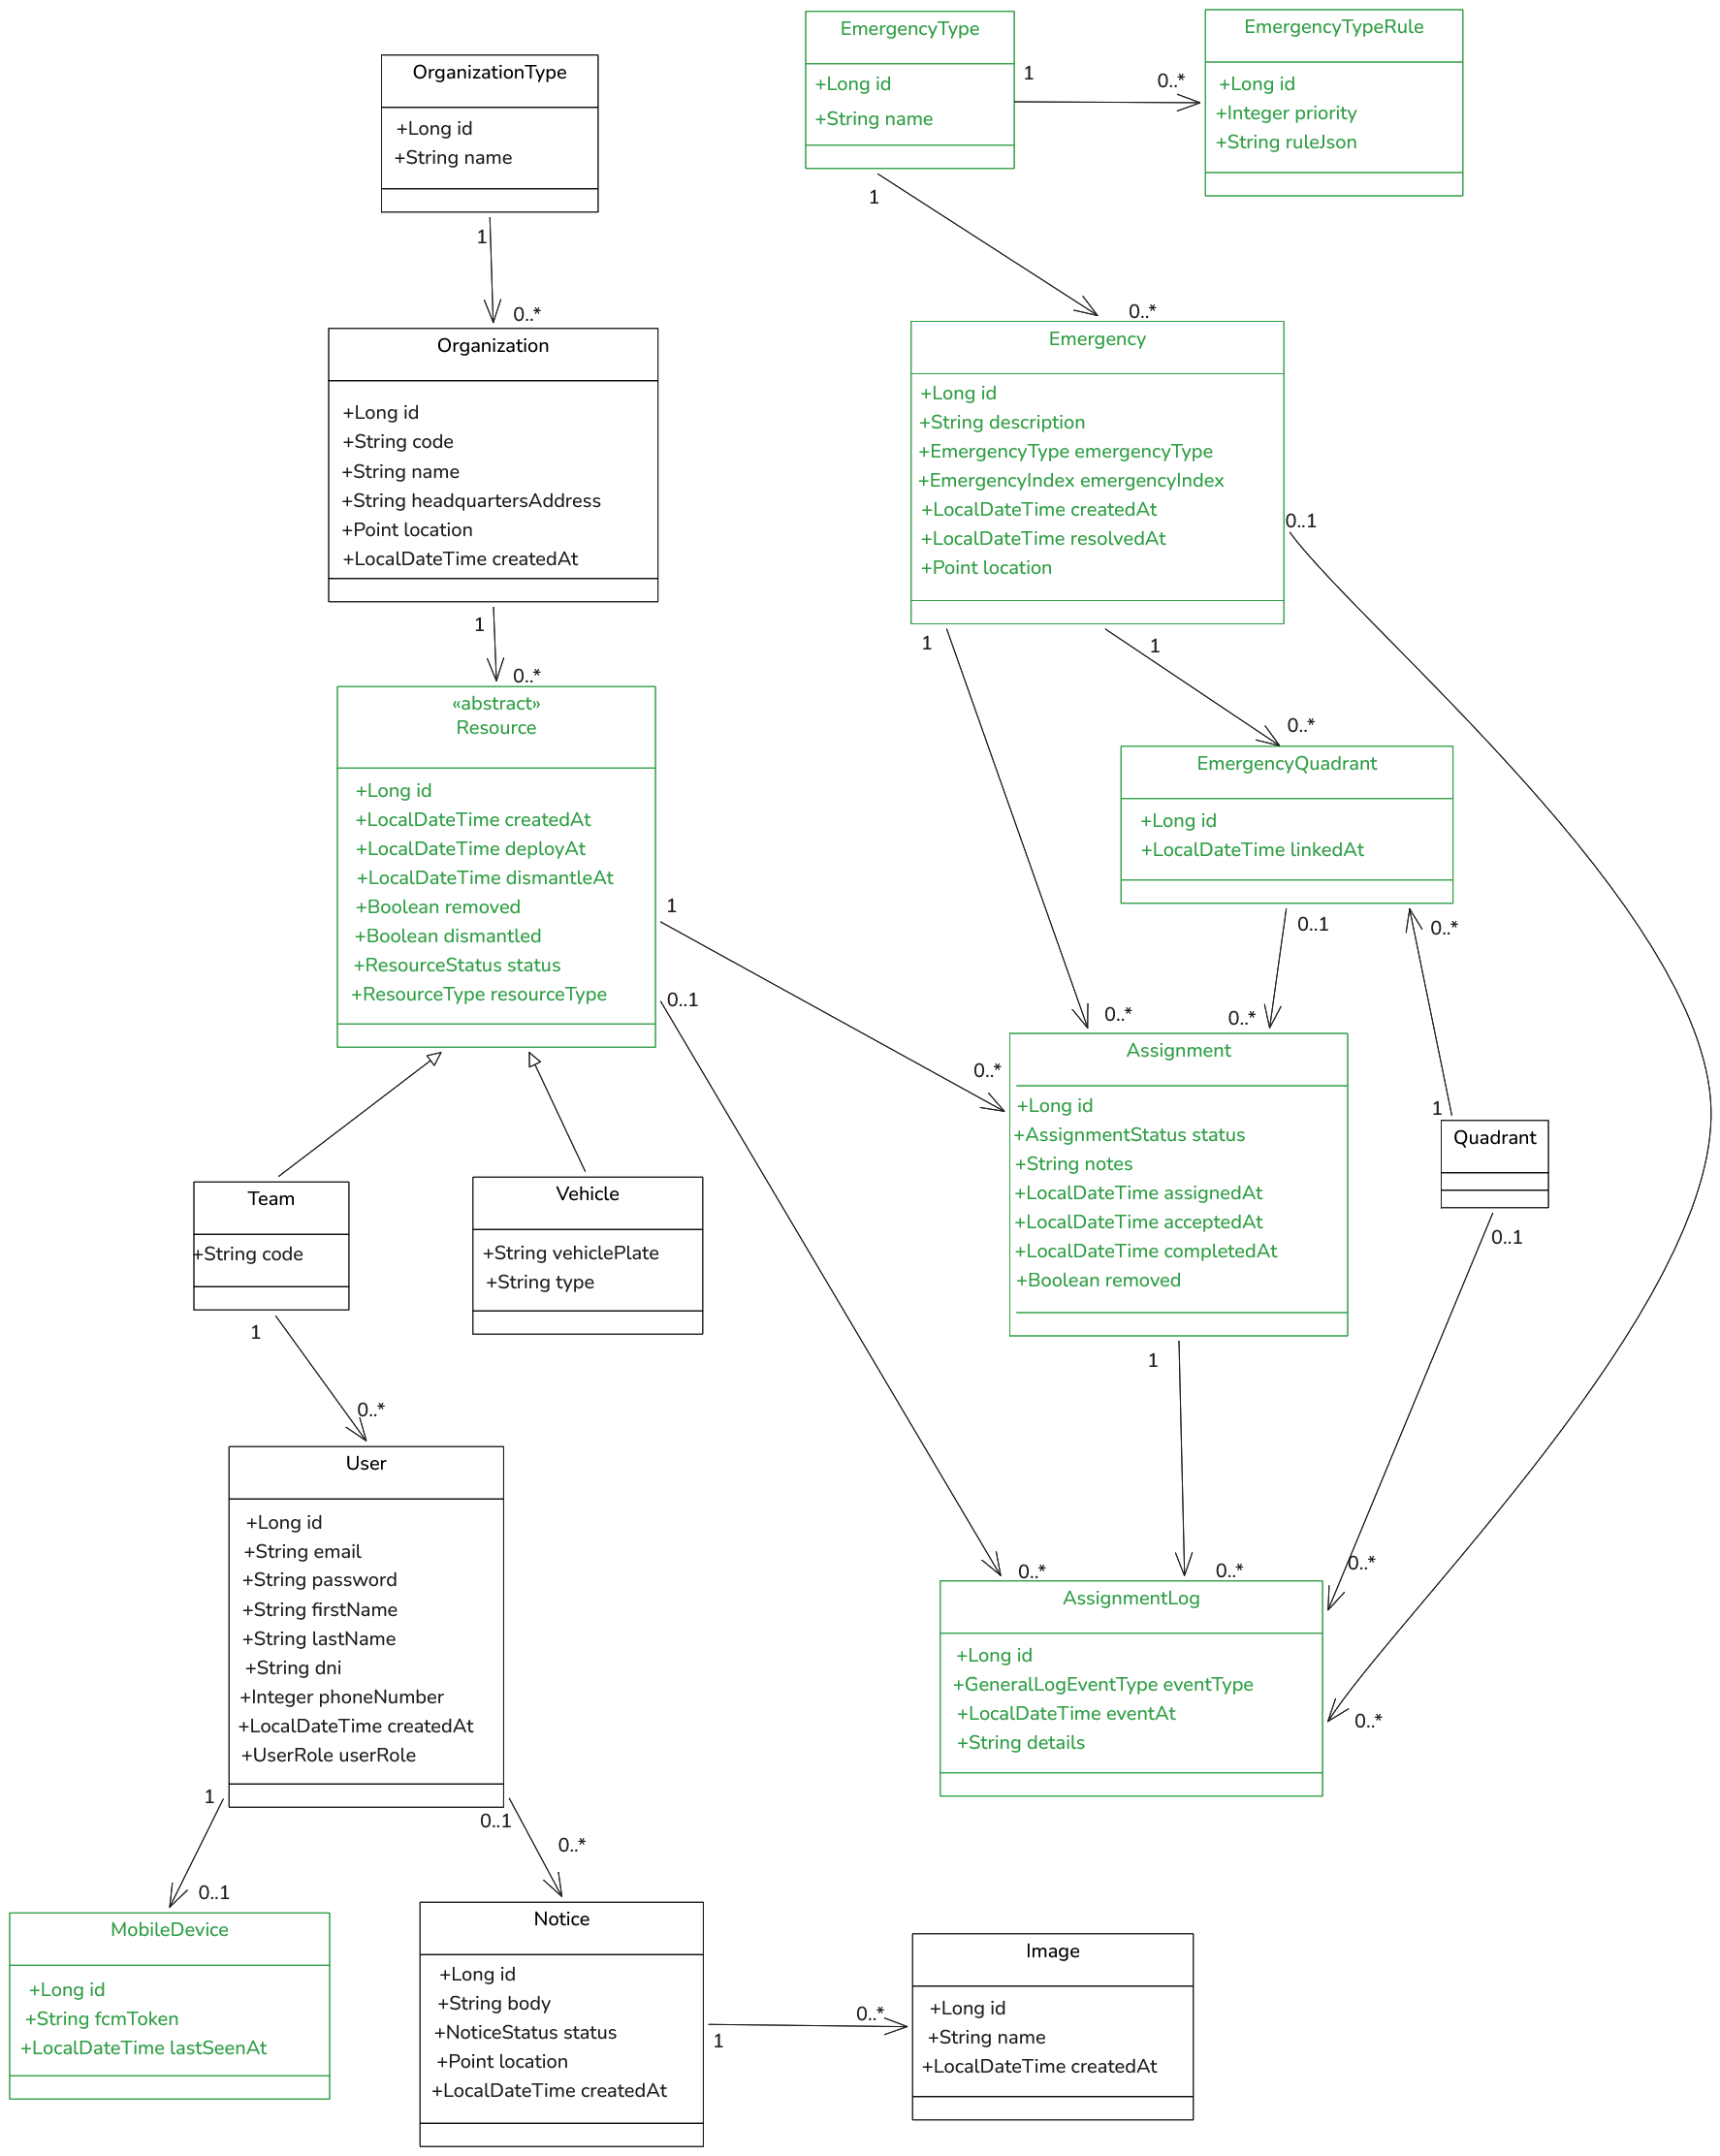
\includegraphics[width=0.9\textwidth]{imaxes/modelo_dominio.png}
  \caption{Diagrama de entidades del modelo de dominio}
  \label{fig:modelo-dominio}
\end{figure}

Frente al trabajo previo, la entidad \textit{Fire} ha sido sustituida por \textit{Emergency}, que amplía el concepto de incidencia y mantiene atributos como descripción, tipo, índice, fechas de creación y resolución, además de admitir tanto localización por punto como vinculación a cuadrantes. Esta ampliación refleja mejor el funcionamiento real de la aplicación, ya que ahora una emergencia puede gestionarse por cuadrantes o por coordenadas.

Otra diferencia relevante es la aparición de \textit{EmergencyQuadrant}, que conserva la relación histórica entre emergencias y cuadrantes con su fecha de vinculación. En la etapa anterior esta información ya existía vinculada al incendio, pero aquí se ha decidido darle una entidad propia para reflejar mejor la evolución de las emergencias a lo largo del tiempo y su relación con los cuadrantes. 

Las asignaciones pasan a tener una entidad propia, \textit{Assignment}, con mayor alcance que en el proyecto anterior. Ahora no solo enlazan recursos con una emergencia, sino que también pueden referirse a un cuadrante concreto o a una emergencia basada en punto, almacenando además su estado, observaciones y marcas temporales del ciclo de vida. Esta ampliación es clave para reflejar los recursos utilizados en las resoluciones de las emergencias.

Los recursos siguen compartiendo la clase base \textit{Resource}, pero su alcance funcional se ha ampliado. \textit{Team} y \textit{Vehicle} heredan de ella y, además de sus datos específicos, ahora participan de forma explícita en el ciclo de despliegue y retirada a través de estados, fechas de despliegue y desmantelamiento y asociaciones con asignaciones. Esto refuerza el papel operativo de ambos tipos de recurso dentro de la aplicación.

En la parte de personal, \textit{User}, \textit{Organization} y \textit{OrganizationType} mantienen la estructura general de la etapa previa, pero su uso se ha ampliado con nuevas relaciones operativas, como la pertenencia a equipos y el registro de dispositivos móviles mediante \textit{MobileDevice}. También se refuerza el papel de \textit{Organization} como contenedor de recursos y unidad de gestión. El bloque de avisos conserva la idea del trabajo anterior con \textit{Notice} e \textit{Image}.

Finalmente, la parte de históricos ya no se apoya únicamente en registros específicos por tipo de recurso, sino en \textit{AssignmentLog}, que unifica la trazabilidad de eventos relacionados con emergencias, cuadrantes y recursos. Esta evolución simplifica la consulta del pasado operativo del sistema y aporta una visión más homogénea de los cambios producidos en la gestión diaria.


\newpage
\subsubsection{Modelo de datos}

El modelo de datos también se ha ampliado de forma notable respecto al trabajo previo. La figura \ref{fig:diagram-bd} resume el esquema relacional actual y permite ver cómo la base de datos ha pasado de una estructura centrada en incendios, recursos y registros históricos separados por tipo a un modelo más homogéneo, orientado a emergencias, asignaciones y trazabilidad operativa.

\begin{figure}[H]
  \centering
  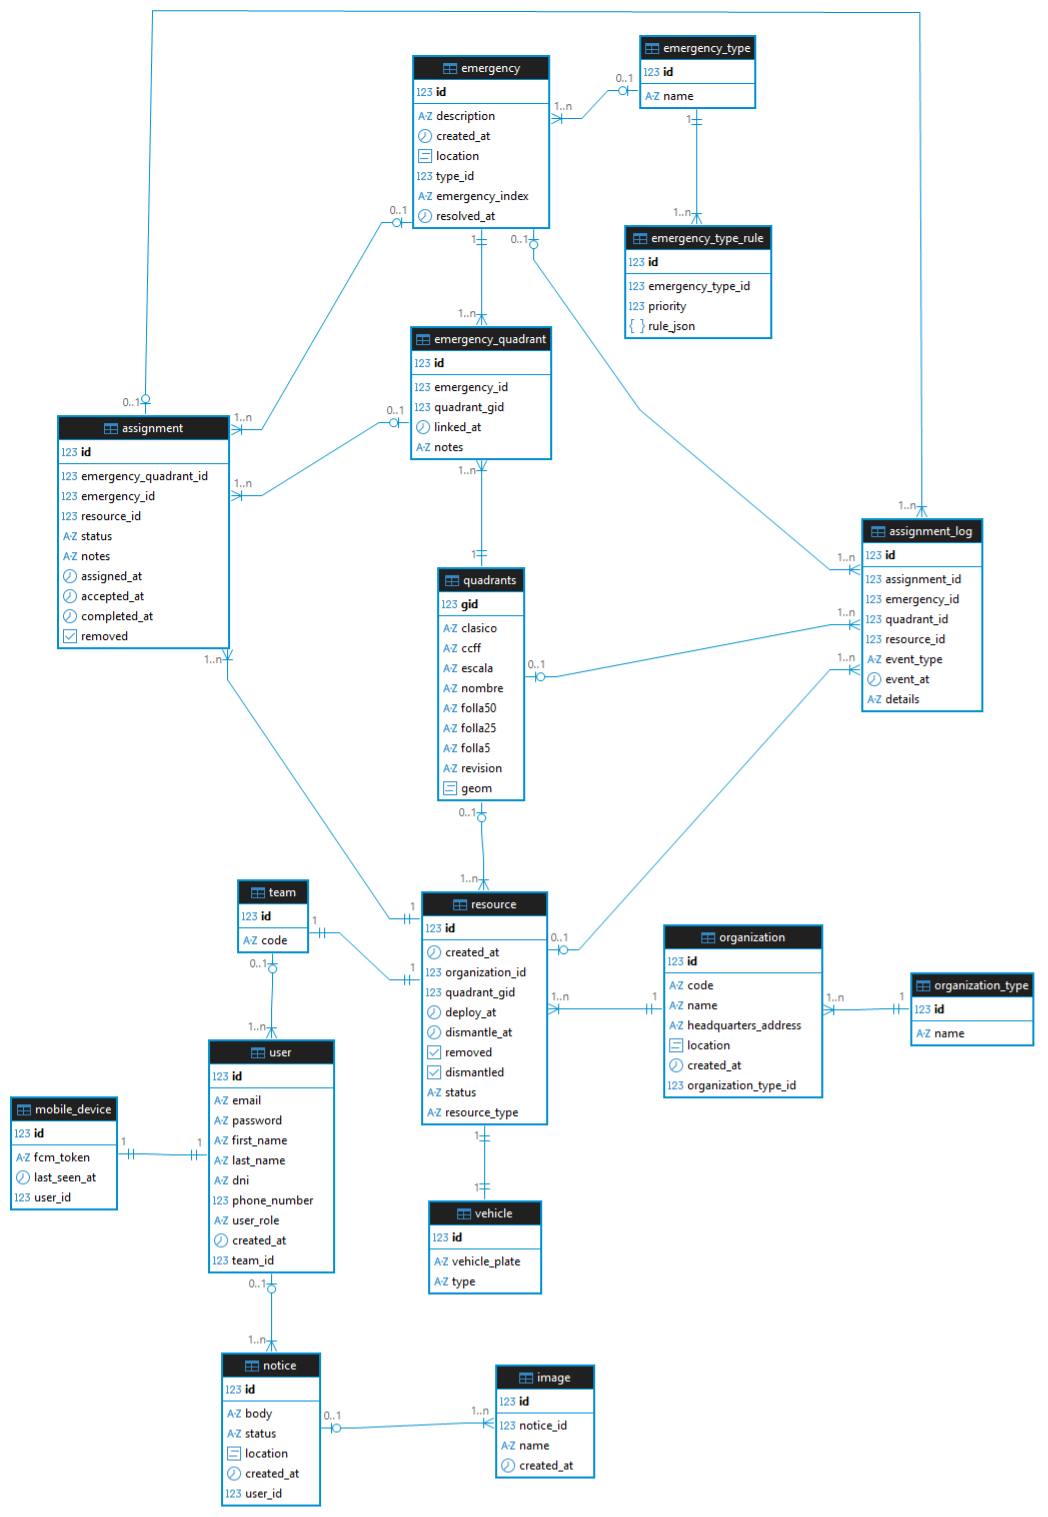
\includegraphics[width=0.82\textwidth]{imaxes/diagram-bd.png}
  \caption{Diagrama relacional de la base de datos}
  \label{fig:diagram-bd}
\end{figure}

En la figura \ref{fig:diagram-bd} se observa que el modelo relacional sigue reproduciendo de forma directa el modelo de dominio, pero con relaciones y tablas adicionales que amplían el alcance funcional del sistema. Frente a la etapa anterior, la aparición de la tabla de \textit{assignment} introduce una entidad central para vincular recursos con emergencias y cuadrantes, mientras que \textit{emergency\_quadrant} consolida la relación entre emergencias y cuadrantes como una relación con histórico propio. Además, se incorpora \textit{emergency\_type\_rule} para almacenar las reglas que alimentan el motor de recomendación, y \textit{mobile\_device} para asociar usuarios con el token FCM utilizado en notificaciones móviles.

También se mantienen las tablas de organizaciones, usuarios, recursos, avisos e imágenes, pero su uso queda ahora integrado en un dominio más amplio. En particular, el antiguo bloque de históricos por recurso se reorganiza alrededor de \textit{assignment\_log}, lo que unifica el registro de eventos y facilita la consulta del pasado operativo. Por último, el modelo conserva campos geoespaciales para almacenar puntos, polígonos y multipolígonos, ya que el sistema sigue trabajando con cuadrantes, localizaciones de emergencias y localizaciones de organizaciones.

\subsubsection{Consideraciones adicionales de modelado de datos}

La mayoría de entidades siguen utilizando claves primarias autogeneradas, lo que simplifica la persistencia y evita lógica manual de asignación de identificadores. Las relaciones entre entidades se definen con anotaciones JPA, principalmente \textit{@ManyToOne}, \textit{@OneToMany} y \textit{@OneToOne}, según la cardinalidad real del dominio.

Se mantiene la política de carga perezosa en las relaciones que pueden crecer en tamaño, como usuarios de un equipo o cuadrantes de una emergencia, pero ahora esa decisión cobra más importancia porque el número de asociaciones ha aumentado. En particular, las relaciones de asignaciones, logs y reglas de recomendación añaden nuevas rutas de navegación entre entidades que conviene cargar solo cuando resultan necesarias.

También se han reforzado las validaciones de Bean Validation, se han añadido restricciones de unicidad y se han definido enumeraciones para campos con valores limitados, como el estado de asignaciones o el tipo de emergencia. Esto afecta tanto a entidades ya existentes, como \textit{Resource} o \textit{User}, como a las nuevas entidades relacionadas con asignaciones y recomendaciones. En \textit{Resource} se centralizan pequeñas reglas de coherencia, por ejemplo el borrado de \textit{deployAt} cuando el recurso vuelve al estado disponible, lo que reduce la dispersión de lógica repetida.

Otro cambio relevante es que en el trabajo anterior la parte de históricos se organizaba por tipo de recurso, con entidades específicas para cada uno. Actualmente se ha optado por un modelo más unificado con \textit{AssignmentLog}, que registra eventos relacionados con asignaciones, emergencias y cuadrantes sin necesidad de separar por tipo de recurso.

\subsection{Capa de acceso a datos}

La capa de acceso a datos se implementa mediante repositorios que extienden \textit{JpaRepository}. Esto proporciona operaciones CRUD sin necesidad de escribir consultas para los casos más comunes. Cuando hace falta un acceso más específico, se añaden métodos derivados por nombre o consultas personalizadas.

El diagrama de la figura \ref{fig:diagram-repository} recoge todos los repositorios del sistema con sus métodos más relevantes. Entre ellos destacan aquellos que incorporan la lógica de acceso más compleja: \textit{AssignmentRepository} combina múltiples criterios de filtrado (cuadrante, emergencia y recurso) en un solo método \texttt{findByFilters}, mientras que \textit{QuadrantRepository} incluye una consulta geoespacial nativa para el cálculo de superficies en hectáreas y una consulta que determina qué cuadrantes tienen emergencias activas. \textit{UserRepository} expone métodos que localizan usuarios por su equipo y rol, necesarios para dirigir las notificaciones push a los miembros del equipo asignado. Por su parte, \textit{TeamRepository} y \textit{VehicleRepository} proporcionan consultas de proximidad geográfica (\texttt{findAvailableClosestToLocation}) que alimentan el motor de recomendación de recursos. El resto de repositorios siguen una estructura más simple, limitándose en su mayoría a las operaciones CRUD heredadas.

\begin{figure}[H]
  \centering
  \includegraphics[width=\textwidth]{imaxes/diagrama-repository.png}
  \caption{Diagrama de repositorios}
  \label{fig:diagram-repository}
\end{figure}


\subsection{Capa de lógica de negocio}

La lógica de negocio se organiza en \textit{facades} e interfaces de servicio, tal como se representa en la figura \ref{fig:diagram-negocio}. \textit{PersonalManagementFacade} agrupa operaciones de organizaciones y usuarios, \textit{ResourceManagementFacade} agrupa equipos y vehículos, \textit{EmergencyManagementService} centraliza las operaciones sobre emergencias y cuadrantes, \textit{AssignmentService} gestiona el ciclo de vida de las asignaciones y \textit{LogManagementService} se encarga de registrar eventos históricos.

En la fachada de personal se gestionan las operaciones de registro, inicio de sesión, edición de perfil, cambio de contraseña, asociación de dispositivos móviles y modificación de roles. En la fachada de recursos, se permiten altas, modificaciones, bajas lógicas y gestión de miembros en equipos. Las organizaciones también se crean y se actualizan desde esta capa.

La parte de emergencias concentra las operaciones de creación, actualización, resolución y vinculación a cuadrantes o puntos. La lógica verifica restricciones de negocio como no modificar una emergencia resuelta o no vincular una emergencia a un punto si ya está asociada a cuadrantes. Como refleja la figura \ref{fig:diagram-negocio}, \textit{EmergencyManagementService} es el servicio con mayor número de operaciones, lo que subraya su papel central en la gestión del sistema.

Junto a estos servicios generales, el diagrama recoge los dos ámbitos más relevantes de la nueva funcionalidad. Por un lado, \textit{AssignmentService} gestiona el ciclo de vida completo de las asignaciones (creación, transiciones de estado y eliminación lógica), apoyándose en \textit{LogManagementService} para registrar cada evento y en \textit{AssignmentNotificationService} para notificar a los miembros del equipo asignado. Por otro lado, los servicios de recomendación (\textit{EmergencyRecommendationService}, \textit{RecommendationRuleManagementService}) implementan el motor de reglas que sugiere recursos de forma semiautomática según el tipo de emergencia y la proximidad geográfica. Estas colaboraciones entre servicios, visibles en la figura, constituyen el núcleo de la nueva lógica de negocio introducida en el proyecto.

\begin{figure}[H]
  \centering
  
\includegraphics[width=\textwidth]{imaxes/diagrama-negocio.png}
  \caption{Diagrama de servicios de lógica de negocio}
  \label{fig:diagram-negocio}
\end{figure}


Las asignaciones son el núcleo más dinámico del sistema. En el siguiente diagrama de secuencia \ref{fig:diagram-assignment} se muestra el flujo de creación de una asignación. El usuario selecciona la emergencia, el cuadrante y el recurso, y envía la petición al backend. \textit{AssignmentService} valida los datos, comprueba que el recurso esté disponible y que la emergencia y el cuadrante existan. Si todo es correcto, se crea la asignación, se registra en el histórico y se envía una notificación al dispositivo móvil del usuario asignado.

\begin{figure}[H]
  \centering
  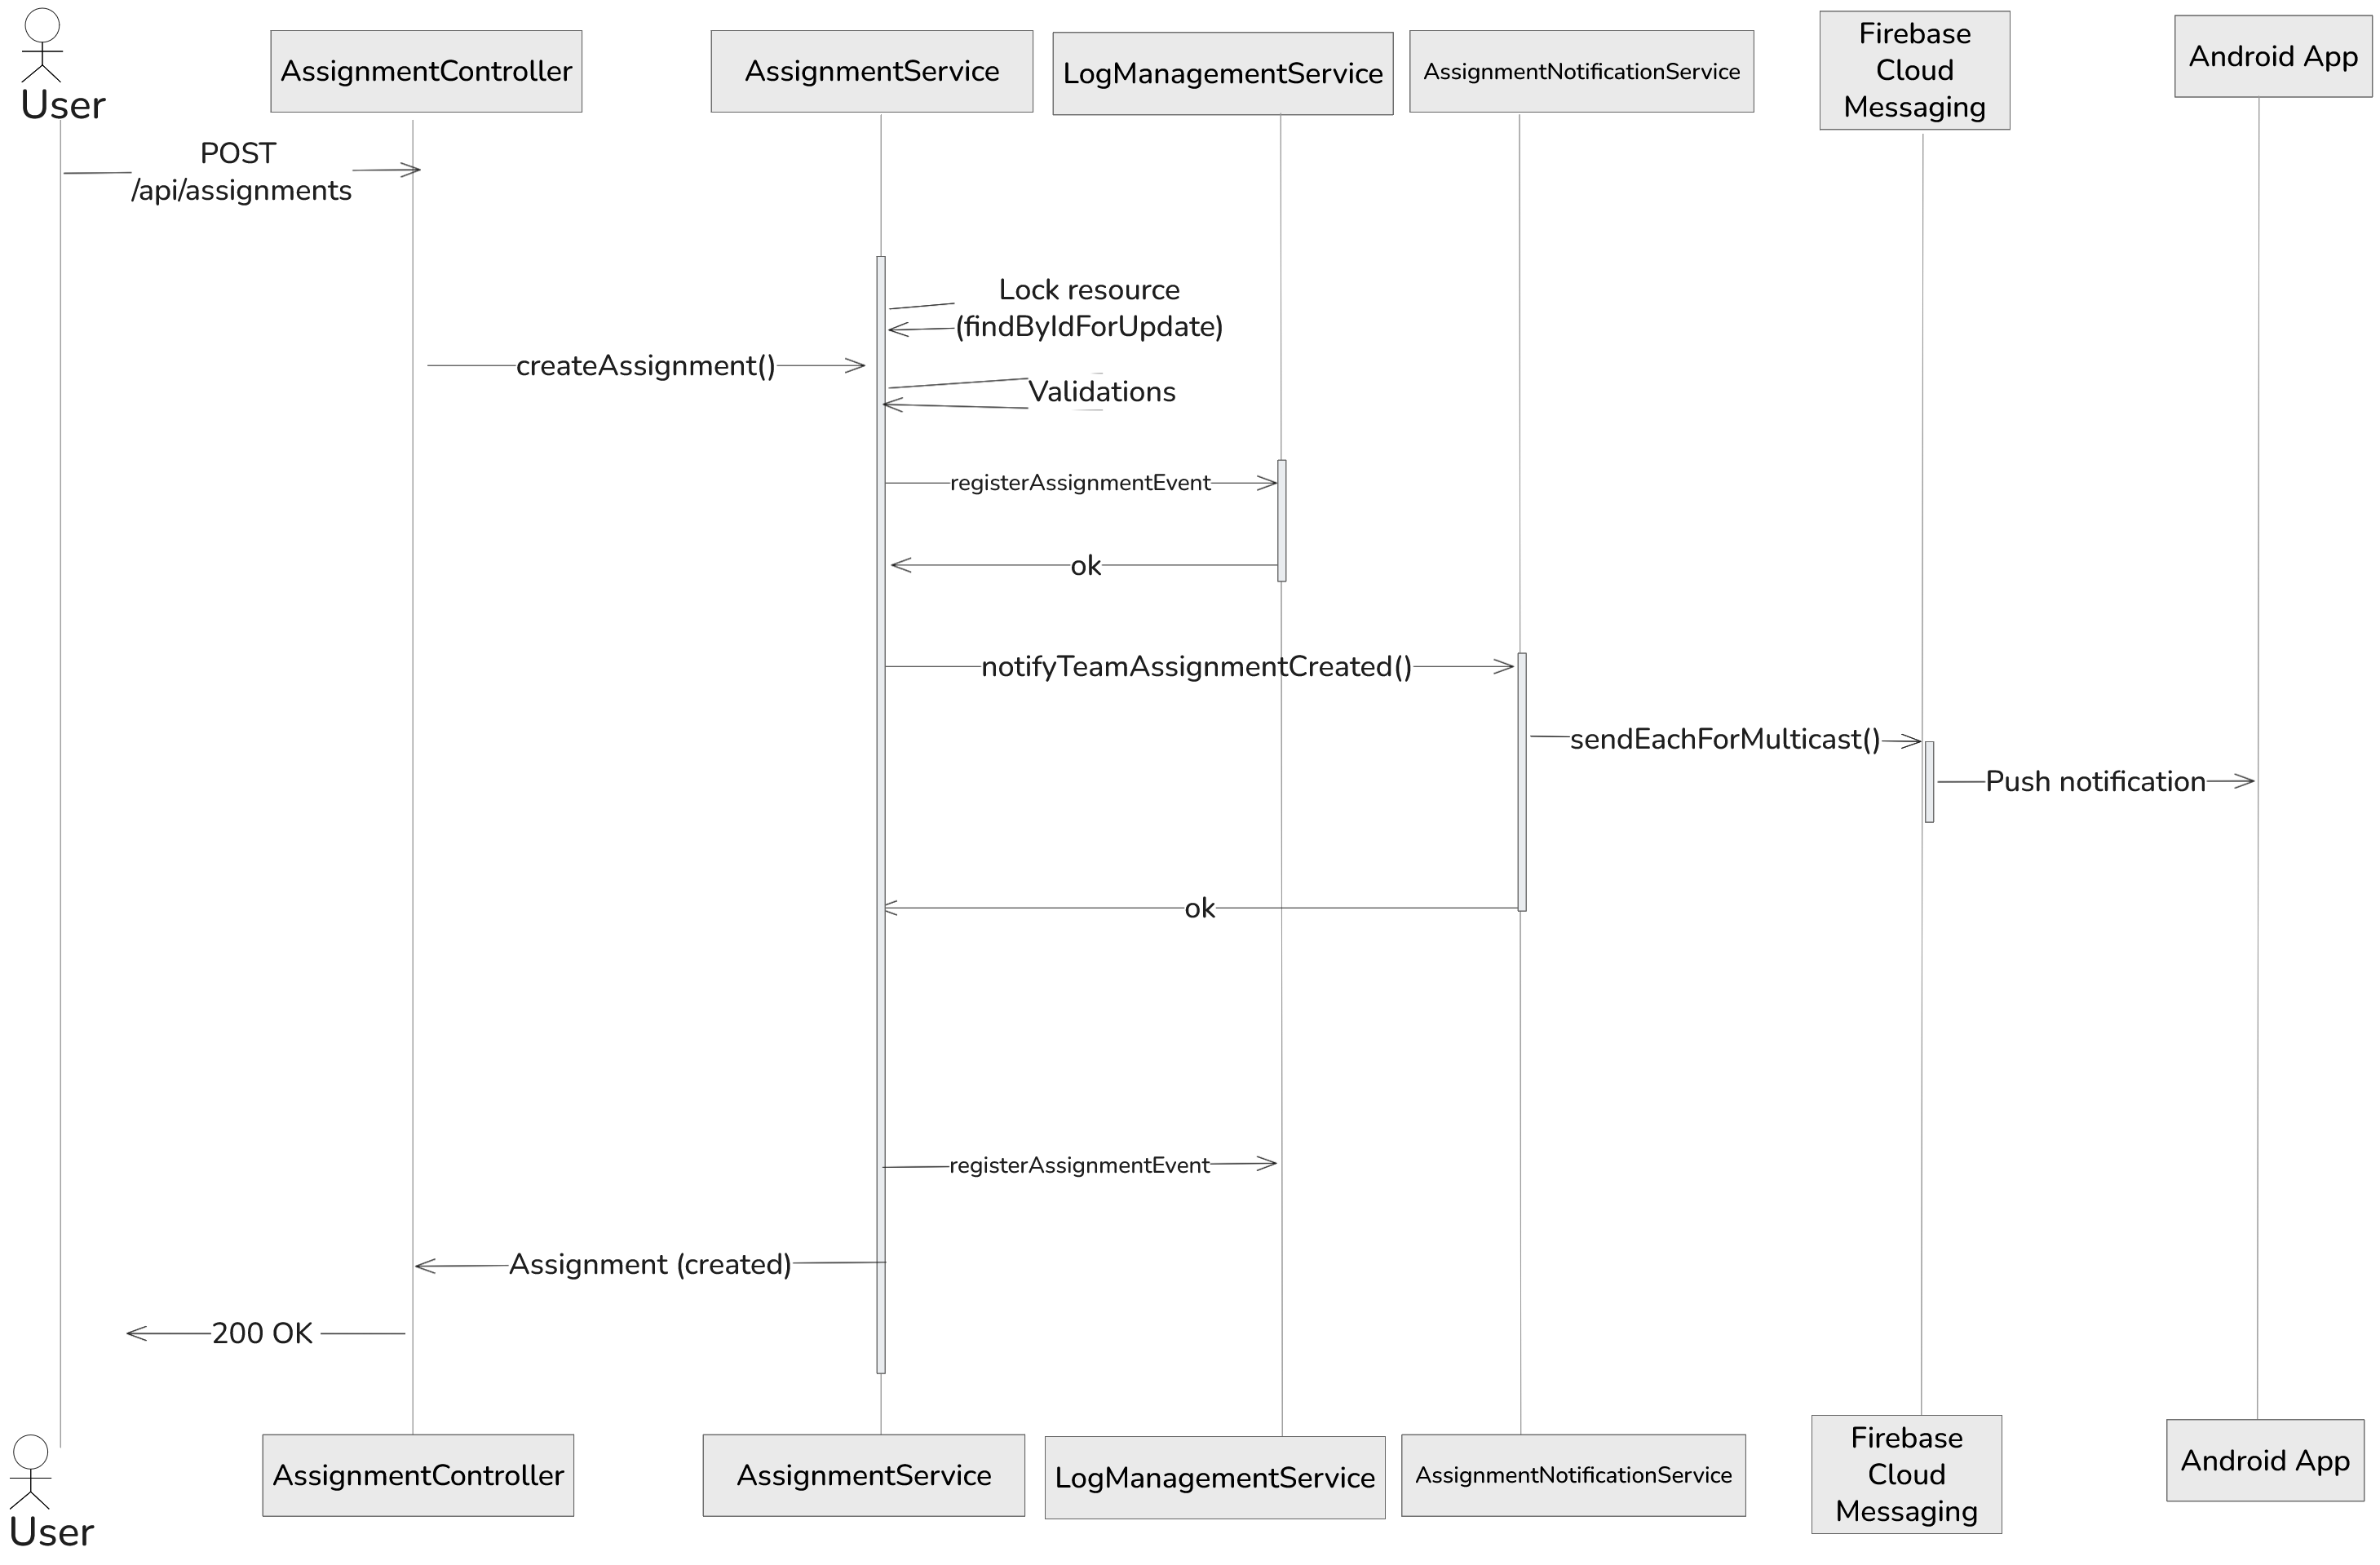
\includegraphics[width=\textwidth]{imaxes/diagrama-secuencia-asignación.png}
  \caption{Diagrama de secuencia de asignación de recursos a una emergencia}
  \label{fig:diagram-assignment}
\end{figure}

Cuando una asignación cambia de estado, el servicio actualiza el recurso asociado, marca la fecha de despliegue o retirada y vuelve a registrar el evento correspondiente. En caso de resolución de la emergencia, las asignaciones pendientes se eliminan lógicamente y las aceptadas se completan automáticamente.

La recomendación semiautomática de recursos se apoya en la entidad \textit{EmergencyTypeRule}, que asocia un tipo de emergencia con una regla en formato JSON estructurado en dos partes: una condición \textit{when} que define el perfil de emergencia (p. ej., tipo concreto, umbral de índice) y una acción \textit{then} que especifica la propuesta (número de equipos, número de vehículos, distancia máxima en kilómetros y tipo de organización preferente). El servicio de edición valida la corrección sintáctica del JSON antes de persistirlo. En tiempo de ejecución, \textit{EmergencyRecommendationService} recupera las reglas ordenadas por prioridad y las evalúa secuencialmente mediante el patrón Chain of Responsibility (descrito en la sección \ref{sec:patrones}); la primera regla cuya condición se cumple determina los parámetros de la recomendación. A partir de ahí, el motor ejecuta consultas de proximidad geográfica (\texttt{findAvailableClosestToLocation}) contra los repositorios de equipos y vehículos para localizar los recursos disponibles más cercanos al punto de la emergencia, aplicando los filtros de distancia máxima y tipo de organización indicados por la regla.

\subsection{Capa de servicios web}

\subsubsection{Diseño de controladores}

Una de las diferencias más importantes es que los controladores se generan a partir de la especificación \textit{OpenAPI}. En la etapa anterior la definición de endpoints dependía de clases controladoras creadas manualmente, mientras que aquí se parte de la descripción de la API y el código generado proporciona la base de las interfaces de controladores y de los contratos de entrada y salida.

Es importante aclarar que se han migrado los endpoints existentes a esta nueva forma de trabajo, lo que ha supuesto un esfuerzo de adaptación pero ha permitido mantener la coherencia en el resto del proyecto. Esta migración es agnóstica respecto a la estructura interna del backend, ya que el código generado se integra con las fachadas y servicios de lógica de negocio sin necesidad de modificar su organización.

Este enfoque reduce errores de sincronización entre documentación e implementación, y facilita que los cambios en la API se propaguen de forma consistente. Los controladores siguen siendo responsables de exponer la operación HTTP, pero la estructura general, los tipos de petición y respuesta y parte de la firma de los endpoints quedan alineados con el contrato definido en \textit{OpenAPI}.

\begin{figure}[H]
  \centering
  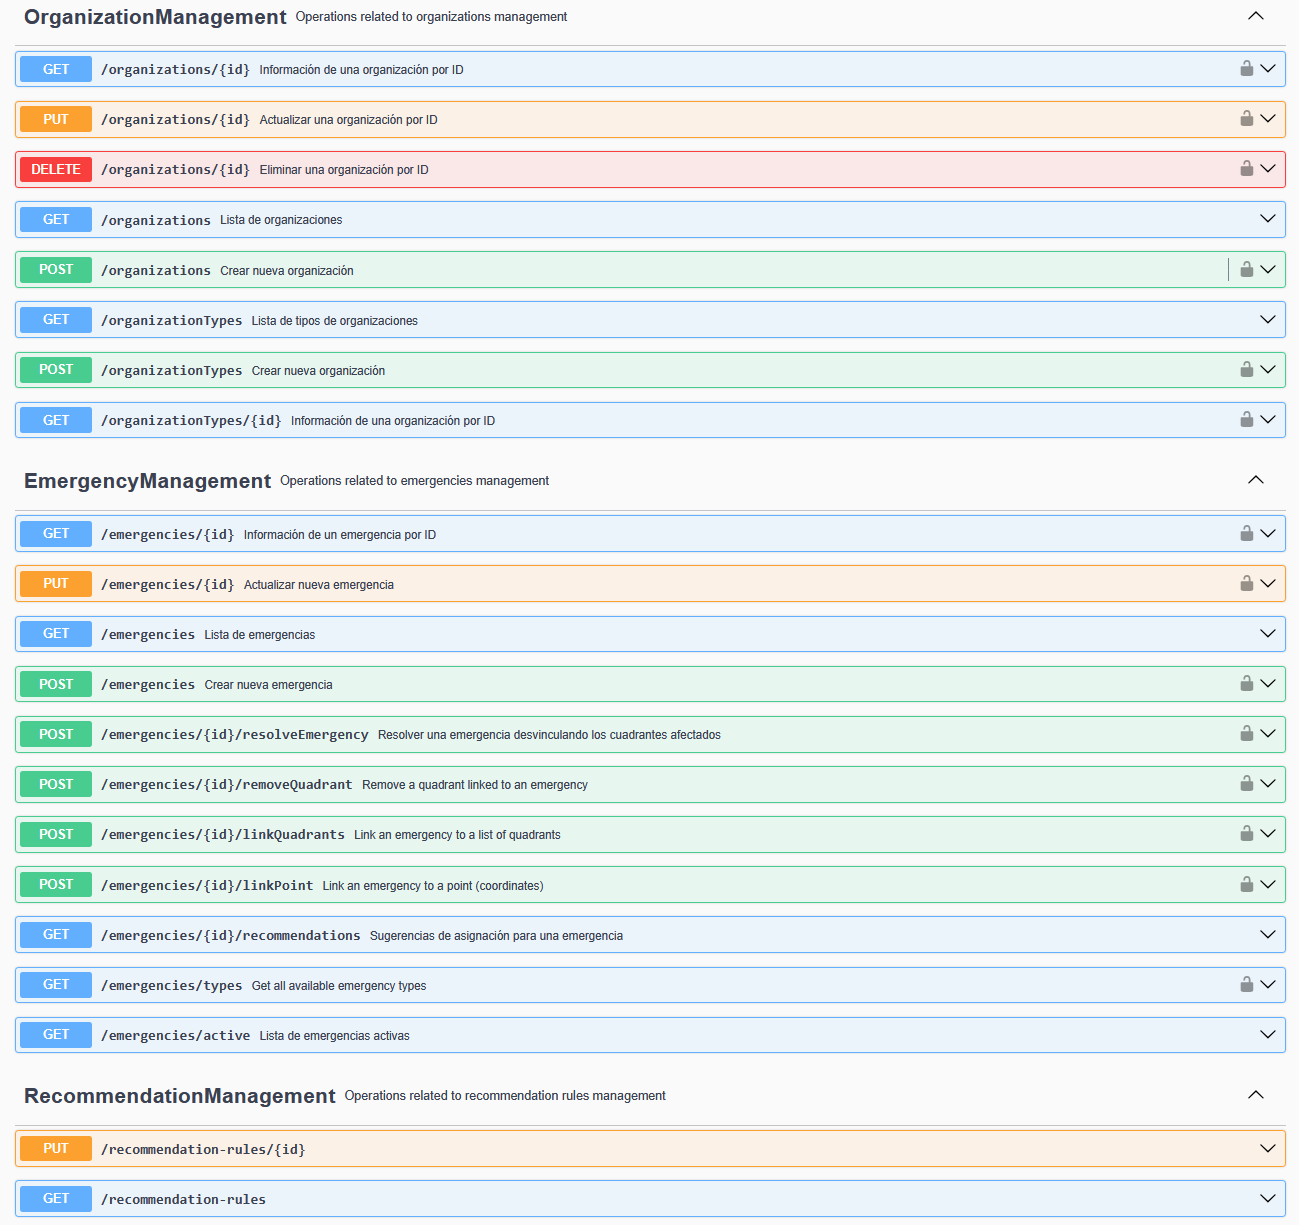
\includegraphics[width=\textwidth]{imaxes/swagger.png}
  \caption{Colección de endpoints documentados en Swagger}
  \label{fig:swagger-collection}
\end{figure}

En la figura \ref{fig:swagger-collection} se muestra la documentación generada mediante Swagger, que refleja los bloques de gestión de organización, de emergencias y de recomendación. El resto de bloques también se ha documentado, pero se han omitido por limitaciones de espacio. En esta vista se observan las ventajas del enfoque \textit{API-first}: la documentación se genera automáticamente a partir del contrato OpenAPI, lo que ayuda a mantenerla sincronizada con la implementación real de los endpoints. Además, permite comprobar de forma centralizada los recursos disponibles, los métodos HTTP asociados y la estructura general de la interfaz pública del backend. También se aprecian los endpoints que requieren autenticación y los accesibles para usuarios anónimos.


\subsubsection{Gestión de errores e internacionalización}

La gestión de errores se centraliza en la clase \textit{GlobalControllerExceptionHandler}. Allí se traducen excepciones de instancia, de dominio y de validación a respuestas HTTP adecuadas y mensajes localizados. Este mecanismo viene del trabajo previo que, con pequeñas adaptaciones, se ha mantenido en la evolución de la aplicación. La internacionalización de mensajes se realiza mediante ficheros de propiedades, y el idioma activo se propaga desde el frontend o la aplicación Android a través de cabeceras HTTP. 

\subsubsection{Control de acceso}

La configuración de seguridad se define en la clase \textit{SecurityConfig}. El backend funciona con sesión sin estado y token JWT. Se autorizan explícitamente los endpoints según el rol: los usuarios anónimos pueden iniciar sesión, registrarse y consultar parte de la información pública; los roles de miembro, gestor y coordinador acceden a recursos y emergencias según sus permisos; y las operaciones de asignación y recomendación quedan restringidas a gestores y coordinadores.

Este bloque también se ha mantenido prácticamente sin cambios estructurales, porque la política de permisos seguía siendo válida para la evolución de la aplicación. La aplicación también registra dispositivos móviles mediante la clase \textit{MobileDevice}, lo que permite enlazar el usuario con su token FCM y habilitar notificaciones push.

\subsection{Librerías y servicios externos}

Además de la persistencia y la seguridad, el backend integra varias librerías y servicios externos. Se usa PostGIS para operaciones geoespaciales, Jackson para el manejo del JSON de reglas de recomendación, y \acrshort{fcm} para notificaciones móviles. También se apoya en una capa de mapeo entre entidades y \textit{DTOs} para desacoplar la API pública del modelo interno.

%%%%%%%%%%%%%%%%%%%%%%%%%%%%%%%%%%%%%%%%
% Subsistema Frontend %
%%%%%%%%%%%%%%%%%%%%%%%%%%%%%%%%%%%%%%%%
\section{Subsistema Frontend}

\begin{figure}[H]
  \centering
  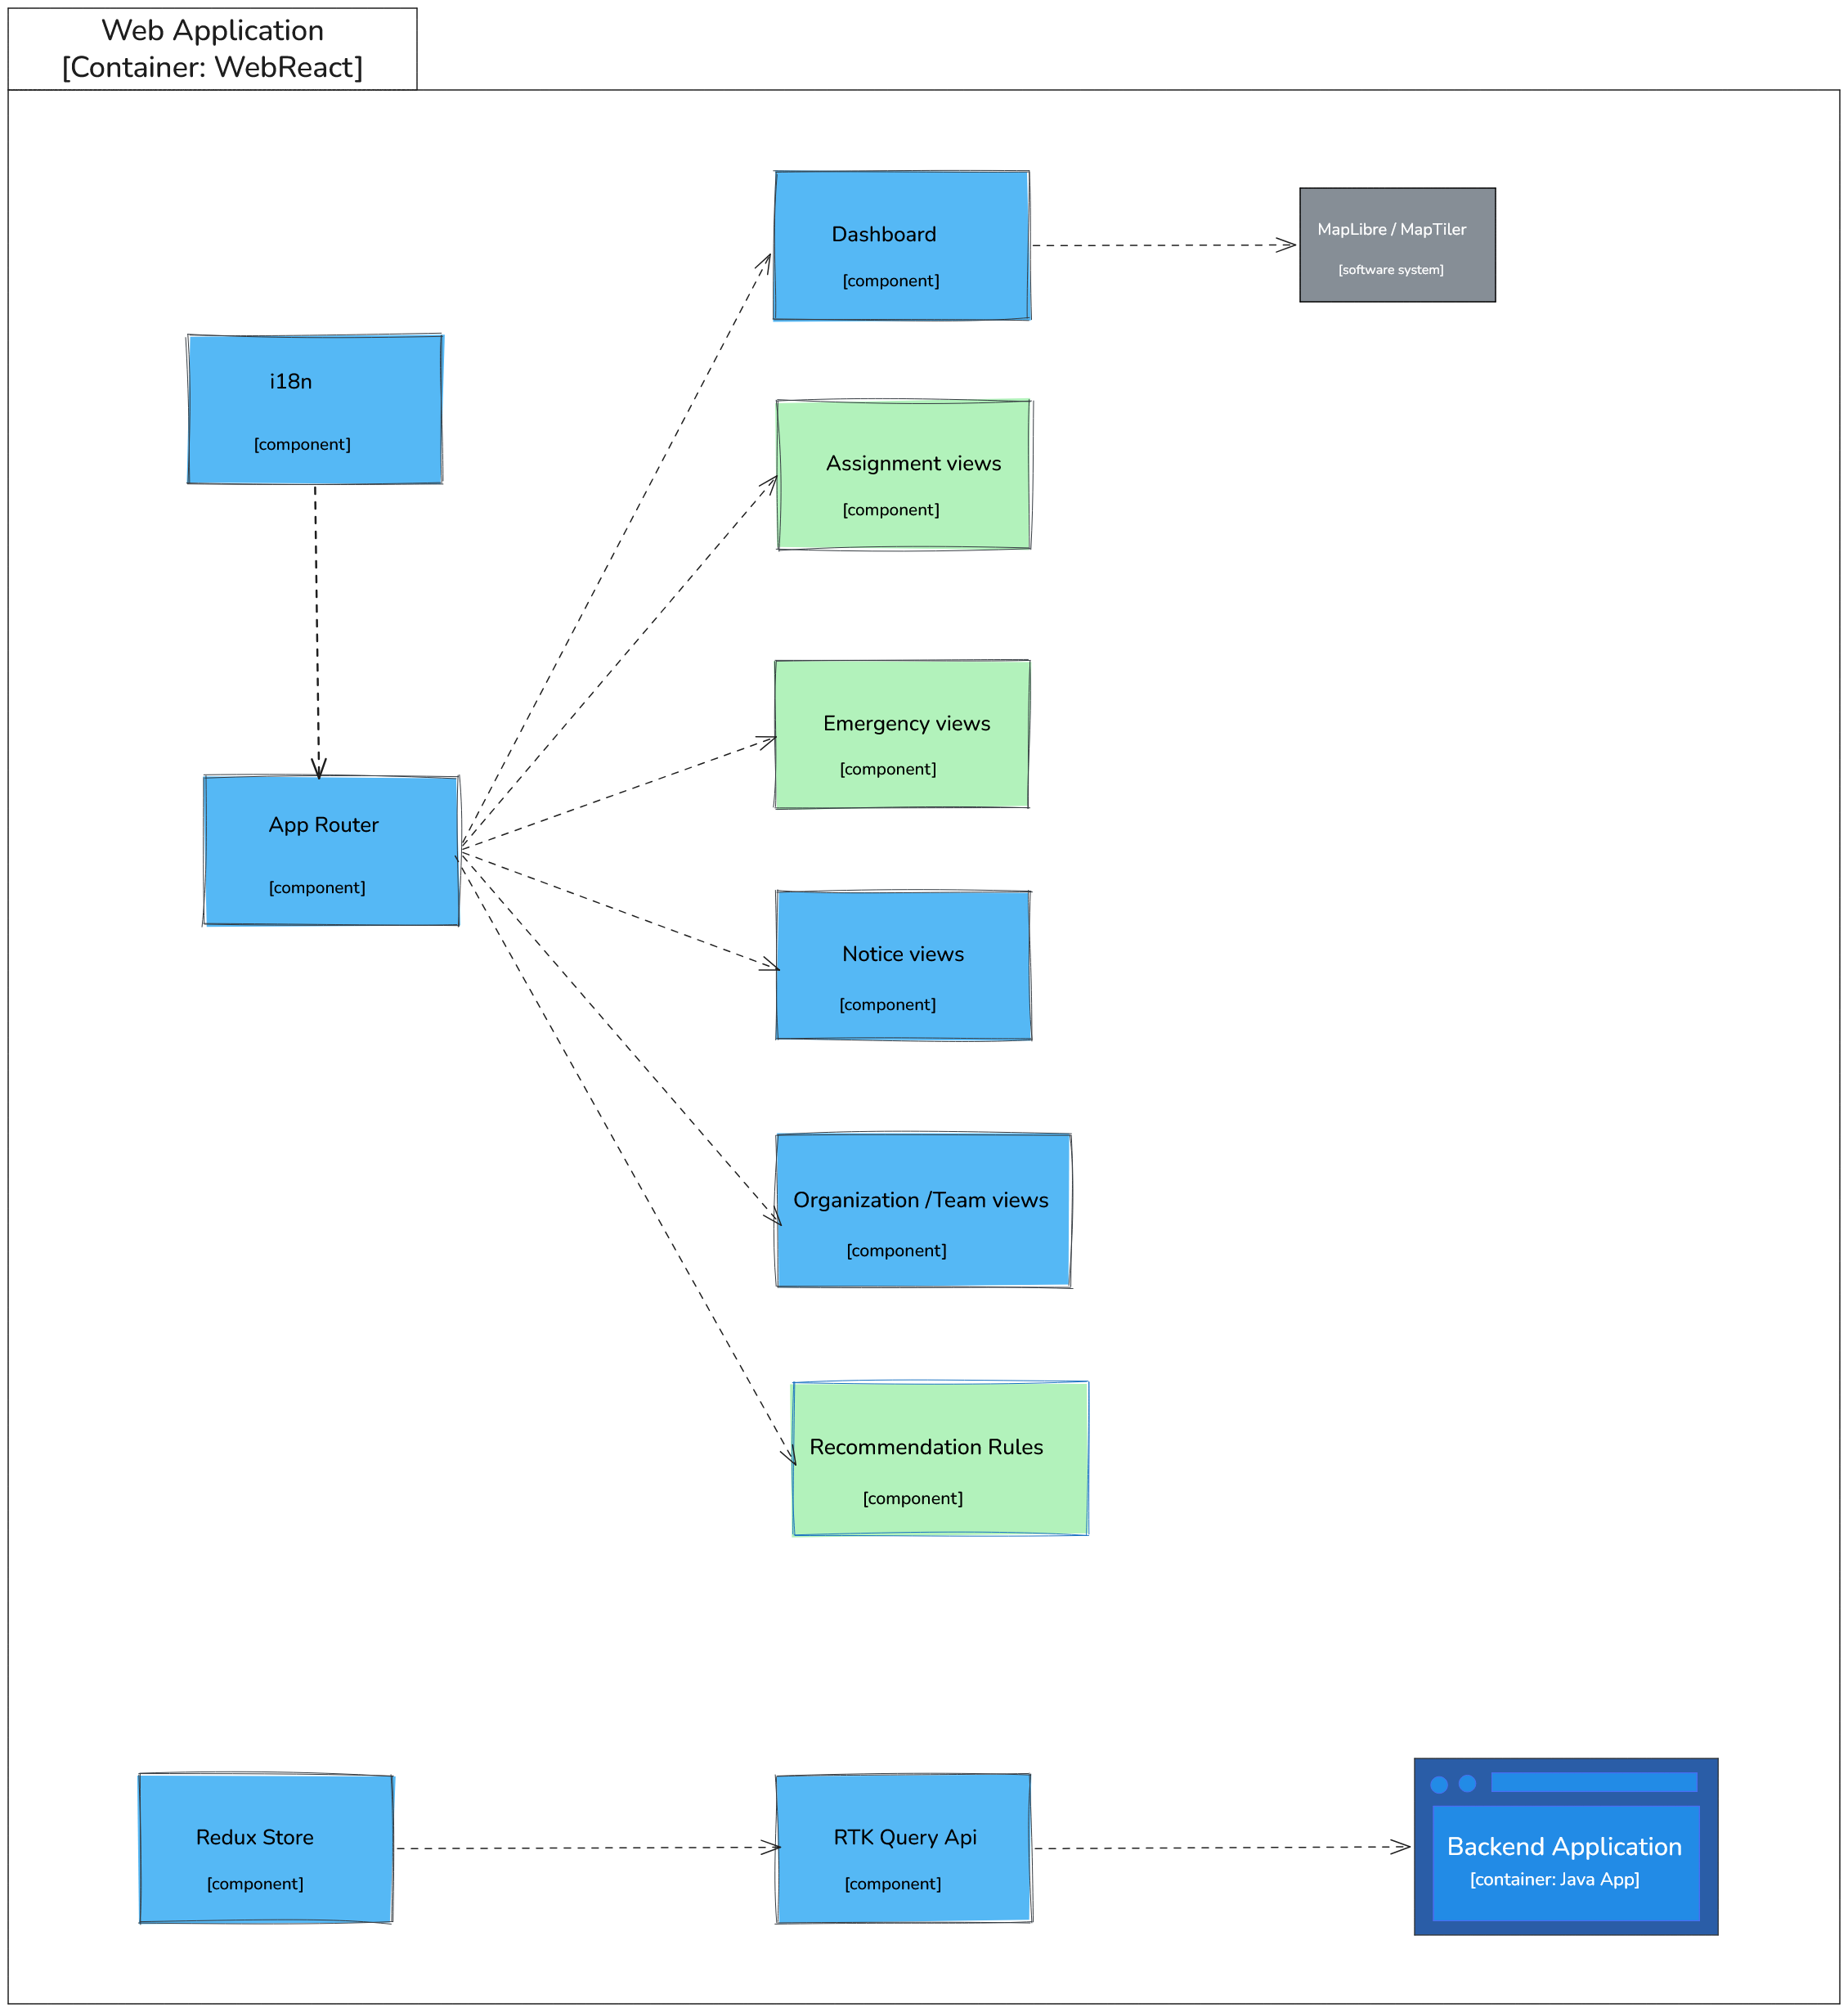
\includegraphics[width=\textwidth]{imaxes/c4/c4_container_frontend.png}
  \caption{Diagrama C4 de contenedores del frontend}
  \label{fig:c4-container-frontend}
\end{figure}

La interfaz se organiza por dominios funcionales reflejados en el diagrama \ref{fig:c4-container-frontend} y se apoya en un store Redux que separa el estado de sesión, el tema visual y los datos de dominio (emergencias, asignaciones, recursos) en slices independientes. Los componentes nuevos o modificados aparecen resaltados en verde.

El mapa (\textit{LandingMap}) representa cada emergencia con un icono y color distintos según su tipología (incendio, inundación, derrumbe, riesgo industrial) y su estado (activa, resuelta). Los cuadrantes se dibujan como polígonos semitransparentes con borde y relleno diferenciados según si están vinculados a una emergencia activa, y los recursos desplegados se muestran como marcadores adicionales sobre el cuadrante correspondiente. Toda la capa cartográfica se apoya en MapLibre con estilos servidos por MapTiler.

La vista de creación de asignaciones presenta tres selectores encadenados: emergencia, cuadrante (solo si la emergencia lo admite) y recurso disponible. Al seleccionar la emergencia, el frontend filtra los cuadrantes vinculados a ella y, al elegir un recurso, valida visualmente que no esté ocupado mostrando su estado en la interfaz antes de enviar la petición. La vista de reglas de recomendación expone un editor JSON con resaltado de sintaxis básico y validación local antes del envío, además de controles para reordenar la prioridad de las reglas mediante arrastre. Los listados de emergencias, asignaciones y avisos incorporan filtros combinados por tipo, estado y fechas, todos gestionados como parámetros de ruta para mantener el estado del filtro entre navegaciones.

%%%%%%%%%%%%%%%%%%%%%%%%%%%%%%%%%%%%%%%%
% Subsistema Android %
%%%%%%%%%%%%%%%%%%%%%%%%%%%%%%%%%%%%%%%%
\section{Subsistema Android}

\subsection{Objetivos}

La aplicación Android complementa al frontend web permitiendo consultar información operativa y ejecutar acciones frecuentes desde el móvil. Debe mostrar mapa, emergencias, organizaciones, perfil, avisos, equipo propio y asignaciones, además de soportar el envío de avisos con imagen y localización.

La interfaz móvil también debe adaptarse al idioma del usuario y mantener coherencia visual con la versión web, aunque con una navegación propia más adecuada al contexto táctil.

Además, la app está pensada como un cliente ligero orientado a la consulta rápida y a la reacción en campo. Por ello concentra en el dispositivo funciones de visualización, notificación y aceptación de asignaciones, mientras delega la lógica de negocio en el backend.

Para mantener la sesión y ciertos parámetros de uso, la aplicación almacena localmente información básica en \textit{SharedPreferences} bajo \textit{app\_prefs}. Ahí se guardan el token JWT, el identificador del usuario, el nombre mostrado, el correo, el teléfono, el DNI, el rol y el idioma activo. Este almacenamiento se usa para restaurar la sesión, aplicar cabeceras de autorización y conservar la configuración lingüística entre ejecuciones.

\subsection{Arquitectura}

La aplicación Android combina una actividad principal con pantallas implementadas en Compose y flujos concretos basados en Activities y Fragments. Desde esa actividad se resuelve la navegación entre pantallas y se mantiene el acceso centralizado al estado de sesión y a las funciones principales.

La aplicación se apoya en una capa de acceso a red centralizada en \textit{HttpClient}, que se encarga de gestionar las peticiones al backend, incluyendo la lectura del token JWT desde preferencias compartidas y la gestión de hosts locales para facilitar el desarrollo. Todas las pantallas reutilizan esa capa para evitar duplicar lógica de conexión, lectura del token y tratamiento del contenido JSON.


La parte de emergencias se apoya en varias pantallas complementarias. \textit{MapScreen} dibuja cuadrantes activos y emergencias sobre MapLibre. \textit{EmergenciesScreen} muestra el listado filtrable de emergencias. \textit{EmergencyDetailScreen} presenta el detalle de una emergencia y, cuando existe localización por punto, consulta el cuadrante correspondiente y recupera las asignaciones vinculadas. \textit{QuadrantResourcesScreen} muestra precisamente esas asignaciones asociadas a una emergencia y a un cuadrante concreto.

La gestión del equipo propio se concentra en \textit{MyTeamCompose} y \textit{MyAssignmentsScreen}. La primera pantalla consulta el equipo del usuario y sus miembros, mientras que la segunda lista las asignaciones pendientes del recurso del usuario y permite aceptarlas desde el propio dispositivo. Este flujo es una de las piezas más relevantes del cliente móvil, porque conecta la notificación recibida con una acción inmediata.

El envío de avisos se mantiene en \textit{SendNoticeFragment}, donde se combinan captura de imagen, obtención de localización y envío al backend. Esta pantalla resume bien el objetivo del cliente móvil: acercar al usuario las acciones que dependen directamente de su situación física.

Las notificaciones push se gestionan mediante \textit{AppFirebaseMessagingService}, que recibe mensajes FCM, crea el canal de notificación, construye la notificación del sistema y redirige al usuario a la pantalla adecuada mediante una ruta interna. Además, el token FCM se sincroniza con el backend al iniciar la actividad principal, de forma que el servidor pueda dirigir correctamente los avisos al dispositivo asociado al usuario.

La aplicación se ha diseñado para ser modular y escalable, de forma que nuevas pantallas o funcionalidades puedan añadirse sin necesidad de modificar la estructura general. Esto se ha logrado manteniendo una separación clara entre la navegación, la interfaz de usuario y la capa de acceso a datos, lo que facilita la evolución del proyecto a medida que se añaden nuevas características o se ajustan las existentes.

\begin{figure}[H]
  \centering
  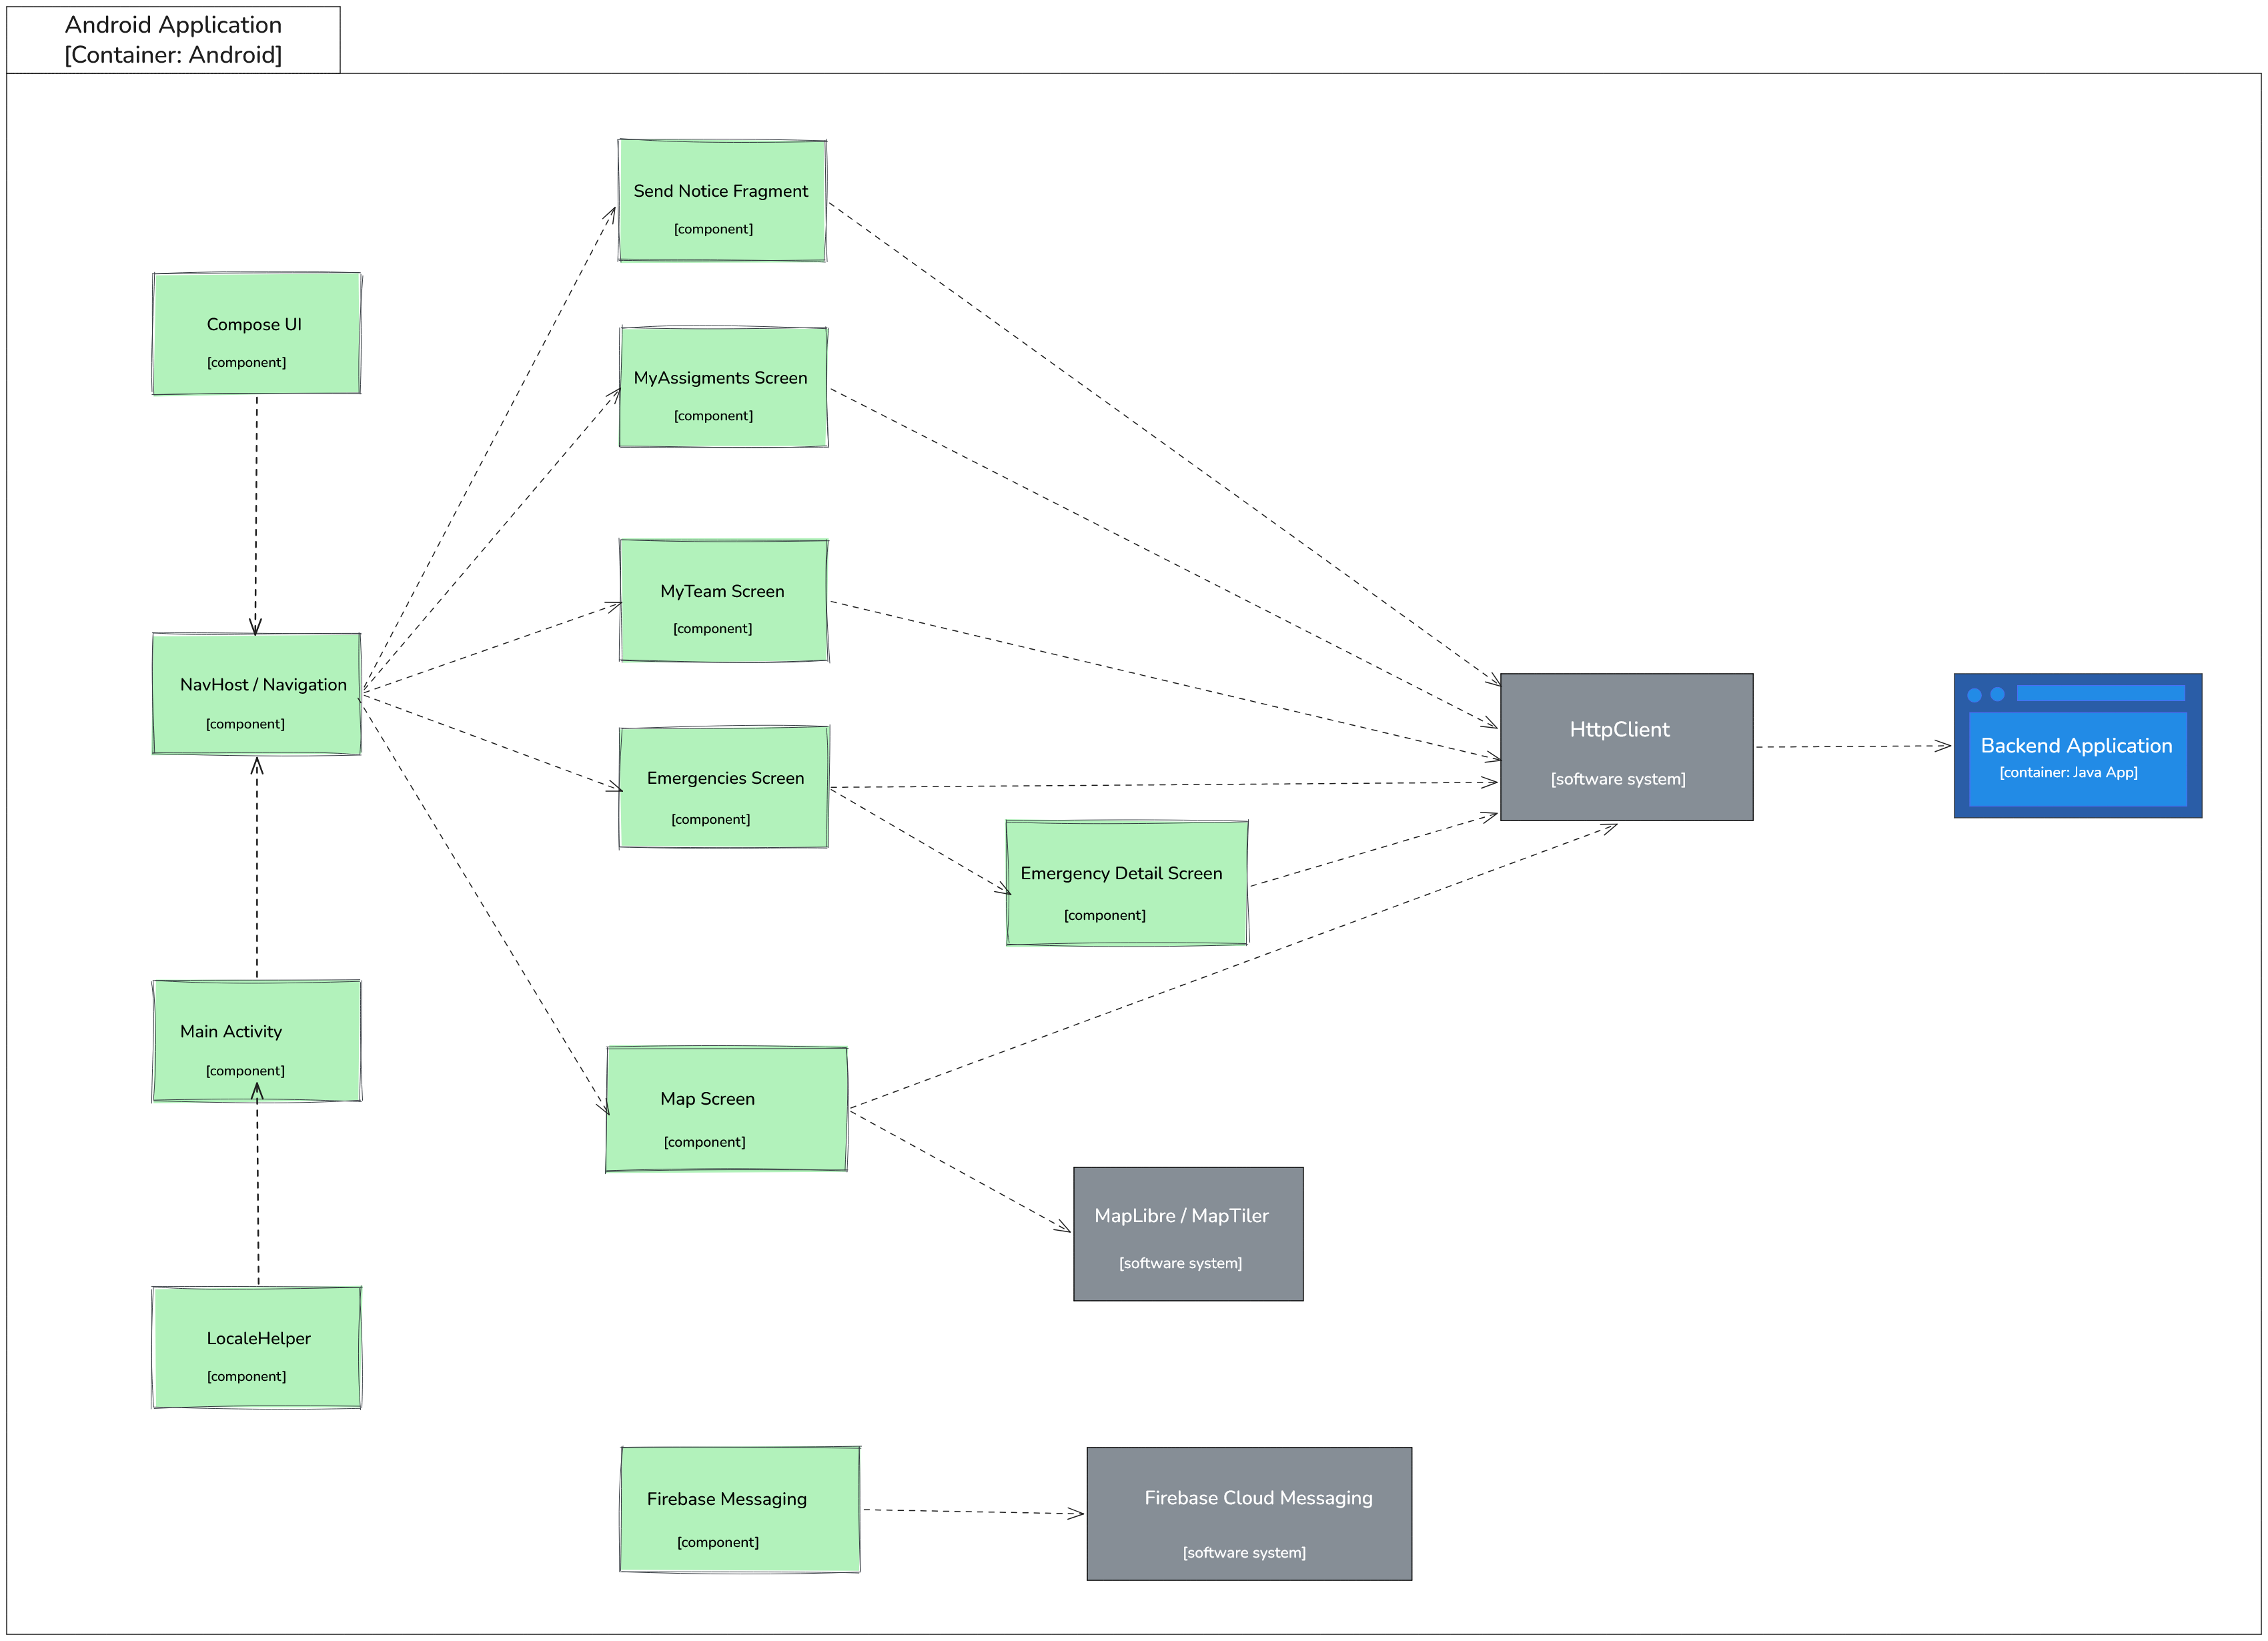
\includegraphics[width=\textwidth]{imaxes/c4/c4_container_android.png}
  \caption{Diagrama C4 de contenedores de Android}
  \label{fig:c4-container-android}
\end{figure}

En la figura \ref{fig:c4-container-android} se muestra la aplicación Android como un contenedor que agrupa navegación, pantallas Compose, accesos puntuales basados en Activities y Fragments, acceso a red, localización, Firebase Messaging e integración con mapas. La vista deja claro que el móvil consume el backend y complementa la interacción con notificaciones y servicios externos.

\subsection{Capa de acceso al servicio}

Las peticiones se realizan mediante \textit{HttpClient}, que resuelve GET y POST contra varios hosts y añade la cabecera de autorización cuando existe sesión. Este diseño simplifica la reutilización y evita repetir código de conexión en cada pantalla.

Las pantallas consumen los mismos recursos del backend que el frontend web, por lo que la capa de acceso se limita a transformar el JSON recibido en estructuras manejables desde Kotlin. En la práctica, esta capa actúa como un adaptador entre el backend y la UI móvil: abstrae la construcción de URLs, reutiliza el token almacenado en preferencias compartidas y centraliza la lógica de reintento sobre varios hosts locales. Esto evita que cada pantalla tenga que implementar su propia comunicación y hace que el acceso a datos sea homogéneo en toda la aplicación.


Como se puede observar en el siguiente diagrama de secuencia \ref{fig:secuencia-httpclient}, cuando el usuario quiere obtener información sobre las emergencias y los recursos asignados a dicha emergencia, el sistema Android realiza una serie de llamadas a la capa REST del backend, a través de la capa de acceso a servicios, para obtener la información necesaria y mostrarla en la interfaz de usuario. El proceso comienza con la pantalla de emergencias, que solicita al backend la lista de emergencias activas. Una vez que el usuario selecciona una emergencia específica, la aplicación realiza una nueva llamada para obtener el detalle de esa emergencia, incluyendo su localización y los cuadrantes asociados. Si la emergencia tiene localización por punto, se realiza una consulta adicional para determinar el cuadrante correspondiente. Finalmente, se recuperan las asignaciones vinculadas a ese cuadrante para mostrar los recursos desplegados en esa emergencia. Este flujo de llamadas garantiza que la información mostrada al usuario esté siempre actualizada y refleje el estado real del sistema gestionado por el backend.


\begin{figure}[H]
  \centering
  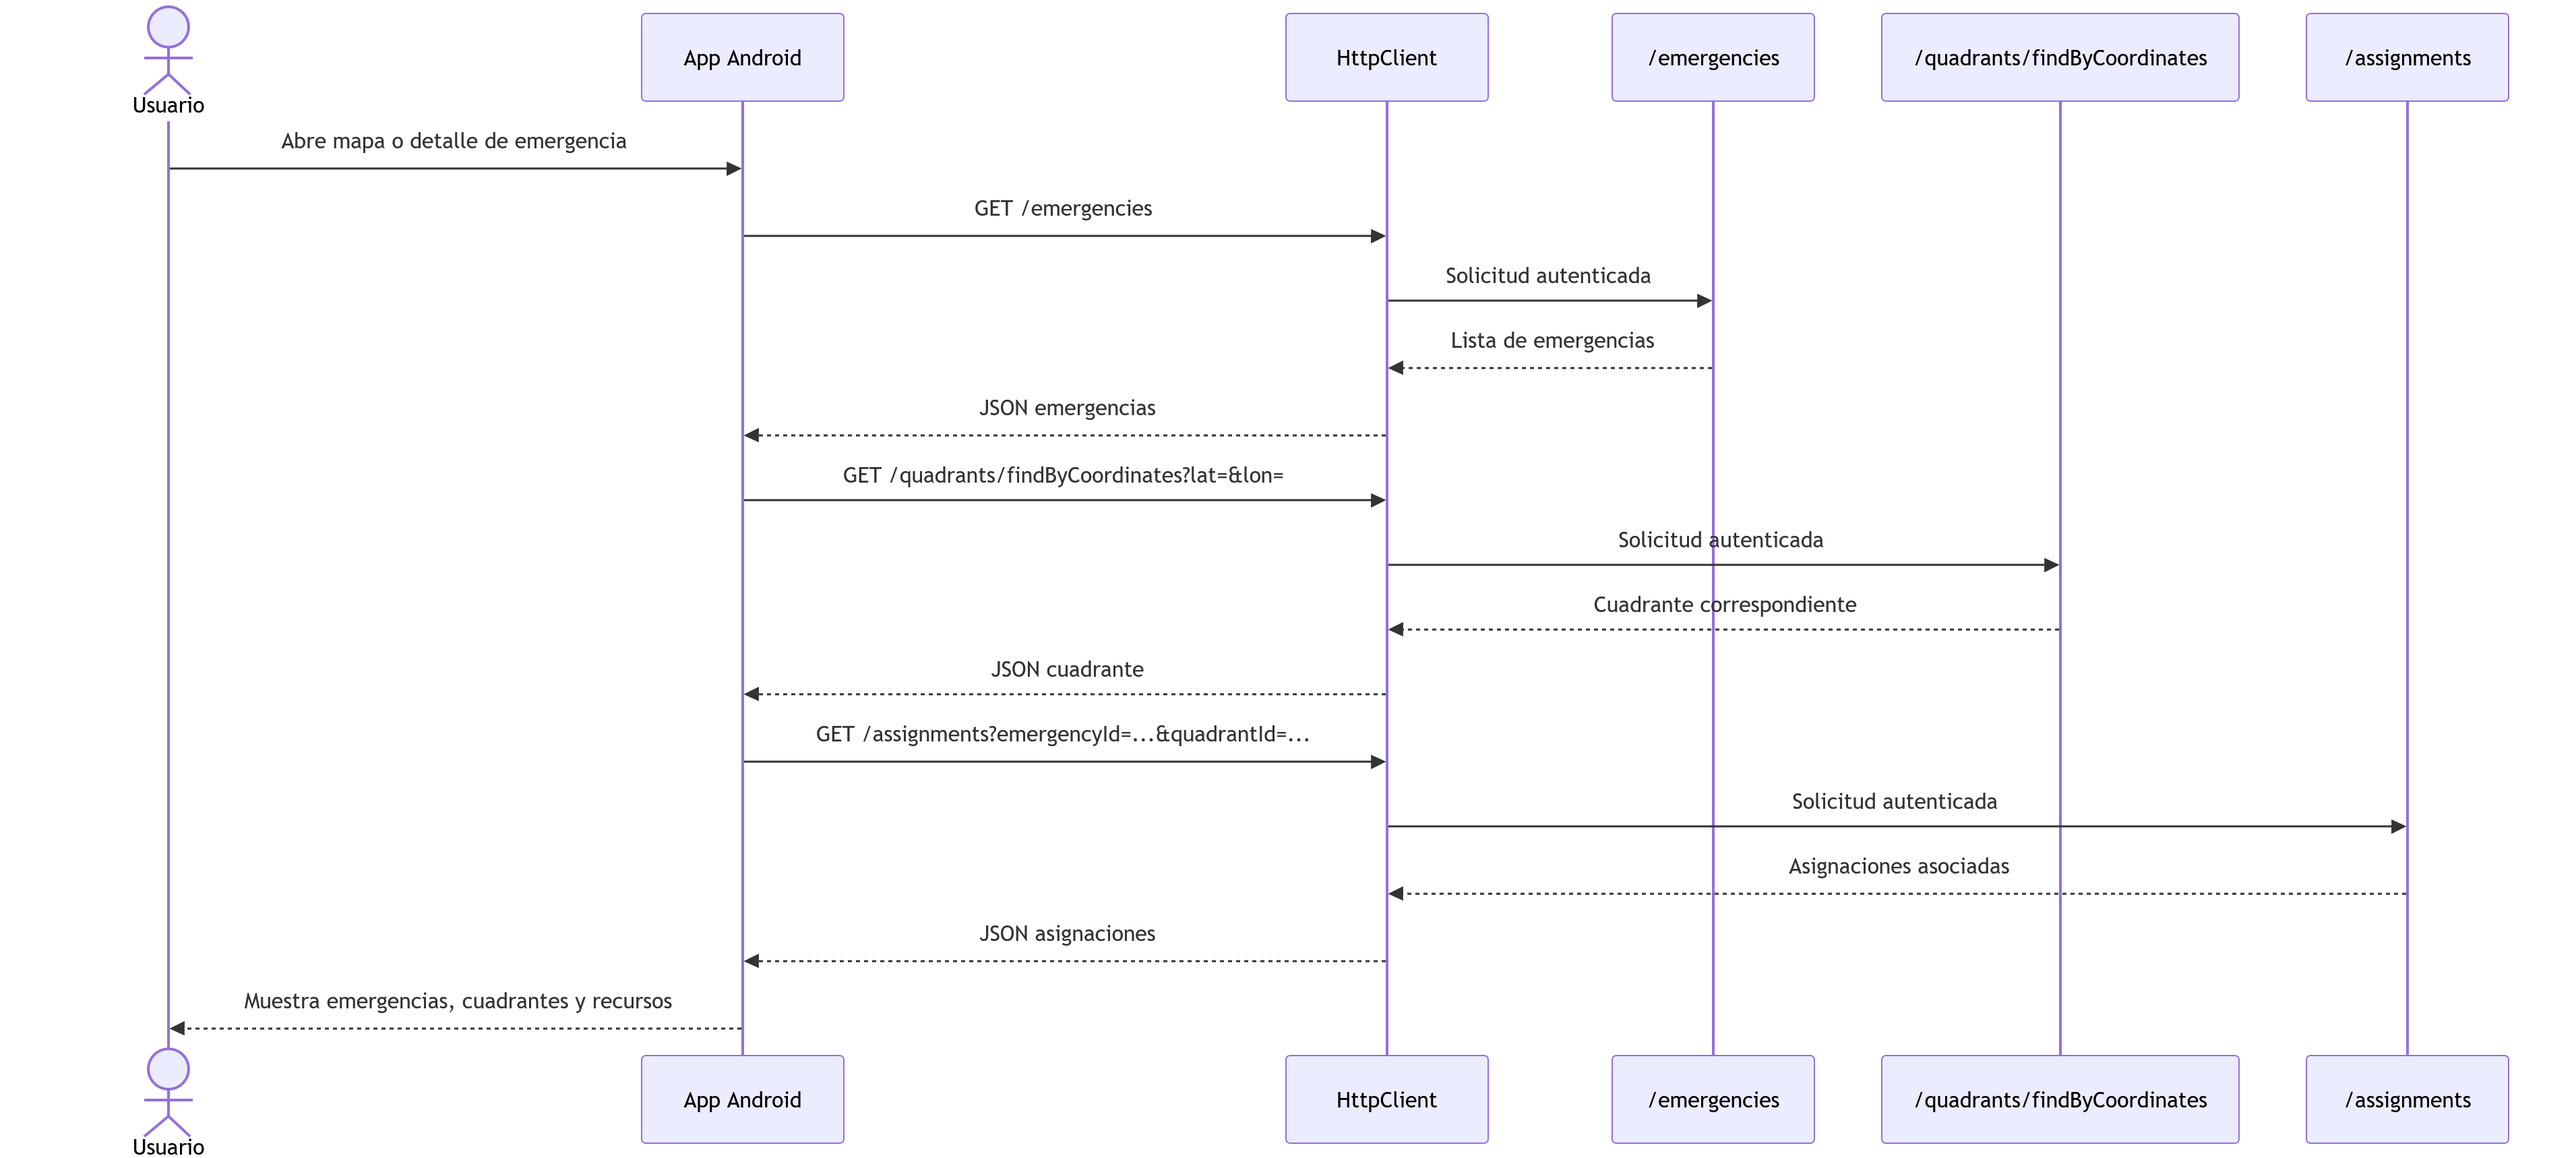
\includegraphics[width=\textwidth]{imaxes/diagrama-secuencia-httpclient.png}
  \caption{Diagrama de secuencia de comunicación entre la capa de acceso a servicios y el backend}
  \label{fig:secuencia-httpclient}
\end{figure}



\subsection{Capa de componentes de interfaz}

La pantalla principal se define en \textit{MainActivity} y su navegación agrupa cuatro bloques principales: mapa, avisos, equipo y gestión. Dentro del contenedor principal, \textit{Scaffold} organiza la barra superior y el menú lateral, mientras que el \textit{NavHost} decide qué pantalla se muestra en cada momento. Esa estructura permite navegar de forma coherente entre las distintas funcionalidades sin abandonar la actividad principal.

\textit{MapScreen} usa MapLibre para mostrar cuadrantes activos y emergencias, y actúa como una vista geoespacial central dentro de la aplicación. \textit{EmergenciesScreen} lista emergencias filtrables y permite abrir su detalle. \textit{EmergencyDetailScreen} muestra la información de la emergencia, los cuadrantes vinculados y los recursos asociados, por lo que concentra buena parte de la navegación operativa. Cuando la emergencia está localizada por coordenadas, la pantalla además calcula el cuadrante correspondiente y consulta las asignaciones asociadas para ofrecer una visión más precisa del despliegue.

La vista \textit{OrganizationsScreen} permite consultar organizaciones y aplicar filtros por nombre o tipo. \textit{ProfileScreen} muestra los datos del usuario y ofrece cambio de idioma y cierre de sesión. \textit{MyTeamScreen} presenta el equipo del usuario, sus miembros y el acceso a las asignaciones activas. \textit{MyAssignmentsScreen} lista las asignaciones pendientes y permite aceptarlas desde el propio dispositivo cuando el usuario dispone de permisos. Este flujo se apoya en la información almacenada localmente y en la sincronización con el backend para mantener el estado del recurso actualizado.

En esta capa también destaca el comportamiento del menú lateral: si el usuario no ha iniciado sesión se muestra un acceso directo al inicio de sesión, mientras que si existe sesión activa se muestran el avatar, el nombre y los bloques de navegación disponibles según el rol. Además, el menú calcula el número de asignaciones pendientes y lo muestra como indicador, ofreciendo una visión rápida del trabajo pendiente sin entrar en cada pantalla.

El envío de avisos se gestiona en \textit{SendNoticeFragment}, donde se combinan captura de imagen, obtención de localización y envío al backend. Esa pantalla refleja bien el objetivo de la app móvil: acercar al usuario acciones directas y relacionadas con su situación física. 

Otro aspecto relevante de la interfaz Android es la gestión de notificaciones push. Para explicar este proceso se ha incluido un diagrama de secuencia \ref{fig:secuencia-fcm} que resume el flujo desde que el backend envía una notificación FCM hasta que el usuario interactúa con ella. El proceso comienza con el backend generando una asignación y el \textit{AssignmentService} enviando una notificación FCM al dispositivo asociado al usuario asignado. La aplicación Android recibe esa notificación a través de \textit{AppFirebaseMessagingService}, que crea una notificación del sistema con el contenido recibido. Cuando el usuario pulsa sobre la notificación, la aplicación redirige al usuario a la pantalla de detalle de la emergencia asociada a esa asignación, permitiéndole consultar la información relevante y aceptar la asignación si lo desea. Este flujo garantiza que los usuarios estén informados en tiempo real sobre las asignaciones que les afectan y puedan reaccionar de forma inmediata desde su dispositivo móvil.

\begin{figure}[H]
  \centering
  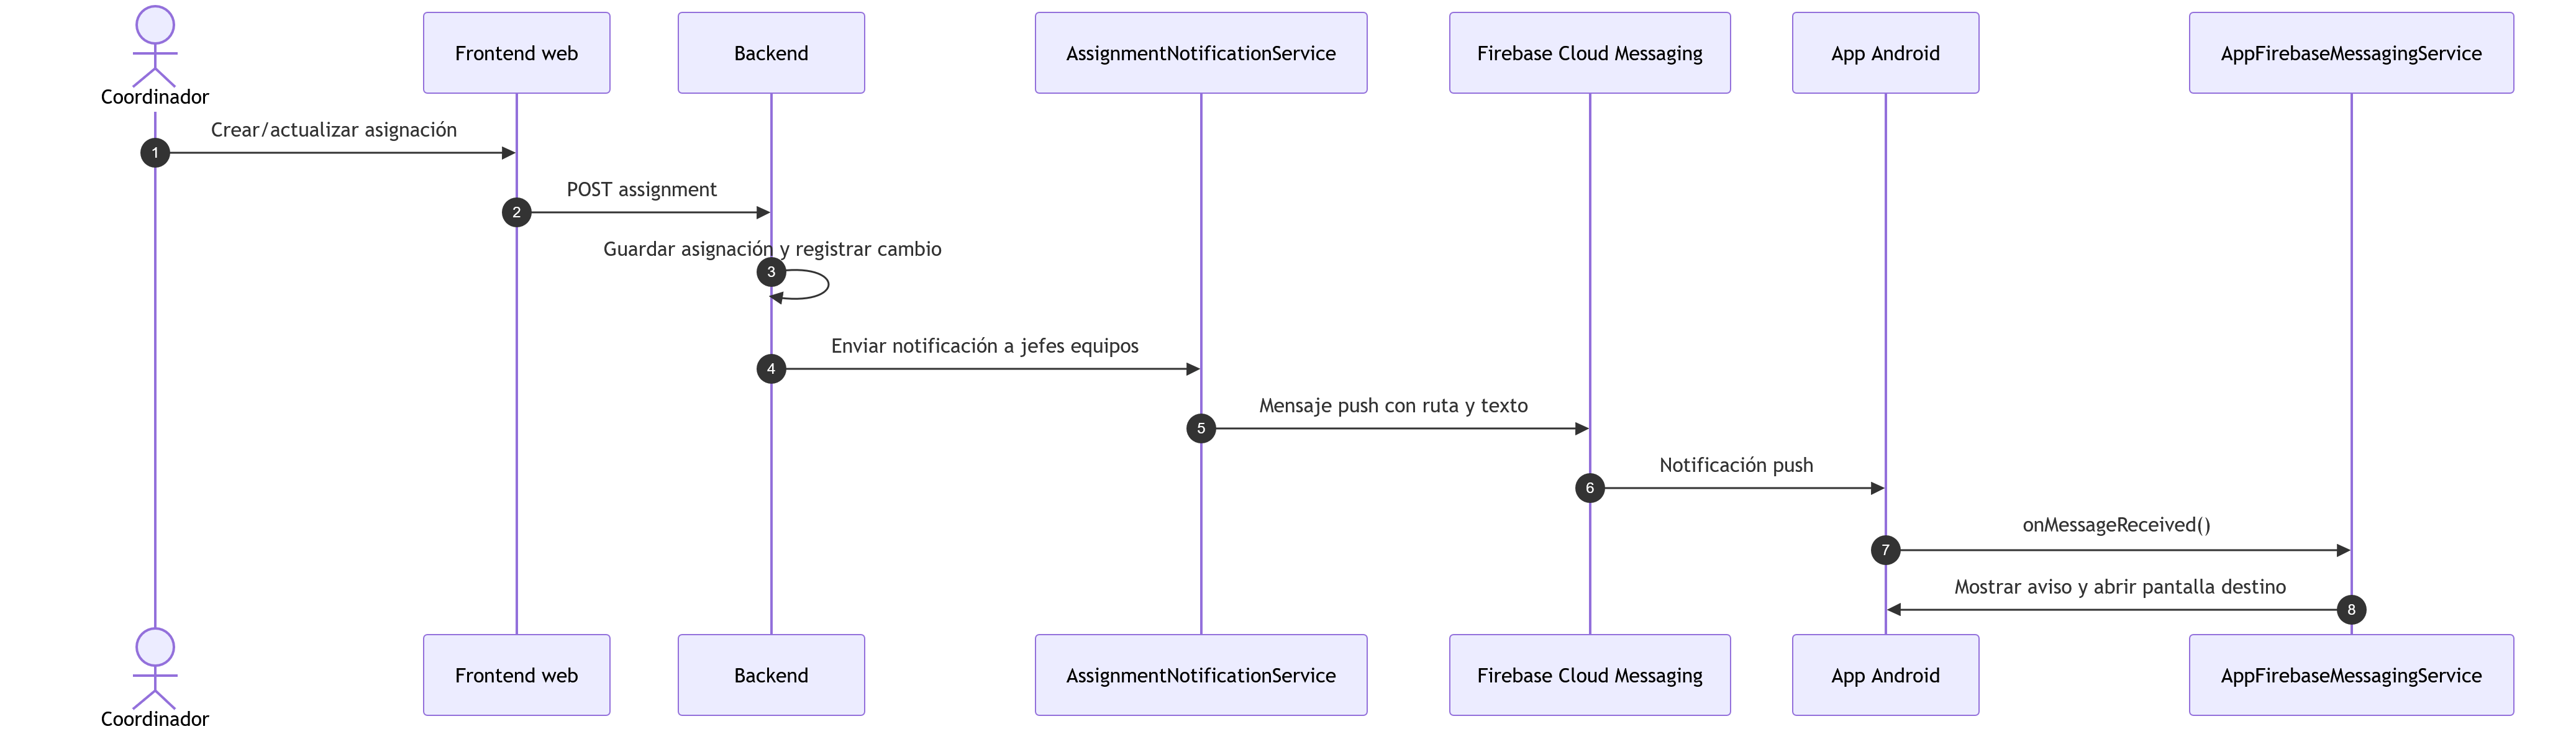
\includegraphics[width=\textwidth]{imaxes/diagrama-secuencia-fcm.png}
  \caption{Diagrama de secuencia de notificaciones FCM en Android}
  \label{fig:secuencia-fcm}
\end{figure}


\subsection{Internacionalización y librerías externas}

La internacionalización móvil se apoya en recursos de cadenas y en un \textit{helper} propio para persistir el idioma activo. La aplicación también integra Firebase Messaging, MapLibre, Glide y Proj4J, además de utilidades para transformar coordenadas entre sistemas geográficos y proyectados.

 \chapter{Implementación}
\label{chap:implementacion}

\lettrine{E}{n} este capítulo se describen los aspectos prácticos de la implementación del sistema, con el objetivo de explicar qué software se necesita para compilarlo, cómo está organizado el código fuente y qué pasos hay que seguir para ejecutarlo en desarrollo.

\section{Software requerido}

Para compilar y ejecutar el proyecto en un entorno de desarrollo es necesario instalar manualmente el siguiente software. El resto de dependencias (Spring Boot, React, MapLibre, Firebase Client, etc.) se descargan automáticamente a través de Maven, npm o Gradle al construir cada subsistema.

\begin{table}[H]
  \centering
  \rowcolors{2}{white}{udcgray!15}
  \begin{tabular}{p{0.28\textwidth}|p{0.28\textwidth}|p{0.28\textwidth}}
    \rowcolor{udcpink!25}
    \textbf{Backend} & \textbf{Frontend} & \textbf{Android} \\
    Java 21 (Eclipse Temurin) & Node.js 18+ y npm & Android Studio \\
    Apache Maven 3.6+ & Git & Android SDK 34+ \\
    Docker y Docker Compose & -- & Git \\
    Git & -- & Configuración local de Firebase \\
  \end{tabular}
  \caption{Software mínimo necesario para levantar cada subsistema}
  \label{tab:software-requerido}
\end{table}

El backend necesita Java 21 con Maven para compilar y ejecutar el servicio. La base de datos PostgreSQL con PostGIS se levanta mediante Docker con el fichero \textit{docker-compose.yaml} incluido en el proyecto, por lo que no es necesario instalar PostgreSQL manualmente.

El frontend solo requiere Node.js 18 o superior y npm para instalar las dependencias de React, Vite y las librerías asociadas.

La aplicación Android necesita Android Studio con el SDK 34, y hay que añadir manualmente el fichero \textit{google-services.json} de Firebase para que las notificaciones push funcionen correctamente.

En los tres casos es necesario disponer de Git para clonar el repositorio. El resto de dependencias se gestionan automáticamente al compilar cada módulo, por lo que no es necesario instalarlas manualmente.

Para la puesta en producción, se recomienda configurar un entorno de despliegue con Docker para el backend y la base de datos, y utilizar servicios como Firebase Hosting para el frontend y Google Play Store para la aplicación Android. Esto viene explicado con más detalle en el apéndice \ref{sec:instalacion}, donde se incluyen las instrucciones de instalación y despliegue de cada subsistema.

\section{Estructura del repositorio}

El repositorio se organiza en tres directorios raíz, cada uno correspondiente a un subsistema: \textit{backend/}, \textit{frontend/} y \textit{EmergencyApp/}. A continuación se describe la organización dentro de cada uno de ellos y los ficheros más relevantes.

\subsection{Backend}

El directorio \textit{backend/} es un proyecto Maven convencional. El código fuente principal se encuentra en \textit{src/main/java}, los recursos (configuración de Spring, scripts DDL, plantillas) en \textit{src/main/resources}, y los tests en \textit{src/test/java}. Dentro de \textit{resources} destacan dos subdirectorios propios del proyecto: \textit{openApi/}, que contiene el contrato YAML de la API, y \textit{db/}, con los scripts de creación e inicialización de la base de datos. El fichero \textit{docker-compose.yaml} se encuentra también en \textit{resources} y permite levantar PostgreSQL con PostGIS en un contenedor. El \textit{pom.xml} declarado en la raíz gestiona las dependencias, el plugin de OpenAPI y el resto de librerías del backend.

\subsection{Frontend}

El directorio \textit{frontend/} contiene la aplicación React con Vite. El código fuente se ubica en \textit{src/}, con subdirectorios por funcionalidad: \textit{api/} para el acceso al backend mediante RTK Query, \textit{features/} para las pantallas agrupadas por dominio, \textit{app/} para la configuración del almacén Redux y utilidades compartidas, \textit{locales/} para los ficheros de traducción (ES/GL) y \textit{features/map/} para la lógica cartográfica con MapLibre. En la raíz se encuentran \textit{package.json} con las dependencias, \textit{vite.config.js} para la configuración del empaquetador y \textit{index.html} como punto de entrada.

\subsection{Aplicación Android}

El directorio \textit{EmergencyApp/} es un proyecto Gradle. El módulo principal está en \textit{app/}, que contiene \textit{src/main/java} con el código Kotlin, \textit{src/main/res} con los recursos (cadenas, iconos) y el \textit{AndroidManifest.xml}. Dentro del código fuente, los paquetes se organizan por responsabilidad técnica: \textit{ui/} para las pantallas con Jetpack Compose, \textit{net/} para el cliente HTTP con Ktor, \textit{messaging/} para la integración con Firebase Cloud Messaging, \textit{data/dto/} para los objetos de intercambio con la API y \textit{util/} para funciones auxiliares. Los ficheros \textit{build.gradle.kts} de la raíz y del módulo \textit{app/} gestionan las dependencias del proyecto.

\section{Instrucciones de compilación}

\subsection{Backend}

Para compilar y ejecutar el backend, primero hay que levantar la base de datos local y después generar y compilar el proyecto. El orden recomendado es el siguiente:

\begin{lstlisting}[language=Bash]
cd backend
docker compose -f src/main/resources/docker-compose.yaml up -d
mvn -DskipTests generate-sources compile
mvn spring-boot:run
\end{lstlisting}

El primer comando inicia PostgreSQL con PostGIS. El segundo ejecuta la generación de OpenAPI y compila el proyecto, incluyendo las fuentes generadas. El tercero arranca la aplicación en modo desarrollo. Si se quiere ejecutar la batería de pruebas backend, el comando habitual es `mvn test`.

\subsection{Frontend}

Para ejecutar la interfaz web, basta con instalar las dependencias y lanzar Vite desde el directorio \textit{frontend/}:

\begin{lstlisting}[language=Bash]
cd frontend
npm install
npm run dev
\end{lstlisting}

Este flujo inicia el servidor de desarrollo y permite trabajar sobre la aplicación sin necesidad de generar primero una compilación final. Cuando se quiera validar el resultado de producción, puede utilizarse `npm run build`.

\subsection{Aplicación Android}

La aplicación Android se abre desde Android Studio a partir del directorio \textit{EmergencyApp/}. Antes de ejecutarla es necesario configurar localmente Firebase y disponer del fichero \textit{google-services.json} correspondiente. Una vez importado el proyecto, la aplicación puede lanzarse desde el propio IDE o mediante Gradle:

\begin{lstlisting}[language=Bash]
cd EmergencyApp
.\gradlew.bat assembleDebug
\end{lstlisting}

En la práctica, la ejecución diaria se realiza desde Android Studio, ya que facilita la selección del dispositivo, la depuración y la gestión de permisos. El comando anterior resulta útil para verificar que el módulo compila correctamente desde línea de comandos.

En conjunto, esta organización permite compilar cada subsistema de forma independiente y reproducible, manteniendo separados el backend, la interfaz web y la aplicación móvil.

 \chapter{Pruebas}
\label{chap:probas}

\lettrine{L}{as} pruebas de software constituyen un pilar fundamental para garantizar la calidad, la corrección y la estabilidad del sistema desarrollado. En este proyecto se ha adoptado un enfoque de pruebas automatizadas tanto para el backend como para el frontend, combinando distintos niveles de prueba según la naturaleza de cada subsistema. Para la aplicación Android, dadas las limitaciones de automatización en el entorno de desarrollo, se ha optado por un plan de pruebas manuales. Este capítulo describe la metodología empleada, las tecnologías utilizadas y el detalle de las pruebas realizadas en cada subsistema.

\section{Backend}

Las pruebas del backend se dividen en dos categorías: pruebas unitarias, que verifican la lógica de negocio de forma aislada mediante simulación de dependencias, y pruebas de integración, que comprueban el funcionamiento conjunto de los servicios con una base de datos real. Ambas están totalmente automatizadas y se ejecutan como parte del ciclo de compilación con Maven, lo que permite detectar problemas de regresión de forma temprana.

Tanto las pruebas unitarias como las de integración siguen una serie de convenciones. La nomenclatura de los métodos de prueba respeta el patrón \acrfull{tdd} con las claves \textit{given} (estado inicial), \textit{when} (acción que se prueba) y \textit{then} (resultado esperado). Además, se emplea el patrón \textit{Arrange-Act-Assert} para estructurar cada prueba de forma clara y legible, facilitando la comprensión de su propósito y lógica. 

\subsection{Pruebas unitarias}

Las pruebas unitarias se han implementado con JUnit 5 y Mockito. Este último permite simular los repositorios y dependencias externas de cada servicio, de modo que las pruebas se centran exclusivamente en la lógica de negocio sin involucrar la persistencia ni la base de datos. Esto permite validar casos límite, reglas de negocio y flujos de error de forma rápida y aislada, asegurando que cada unidad de código se comporta correctamente bajo diferentes escenarios. 

Para la creación de entidades de prueba se emplea el patrón \textit{Object Mother}, que proporciona fábricas estáticas con valores por defecto y métodos de personalización, facilitando la creación estándar y a la vez flexible de objetos sin saturar cada prueba con lógica de inicialización.

La siguiente imagen \ref{fig:object-mother} muestra un ejemplo de clase que sigue el patrón Object Mother para la entidad \texttt{Organization}, con métodos estáticos para generar instancias preconfiguradas y personalizables. Este patrón tiene numerosas ventajas como la reutilización de código, mantenibilidad y legibilidad alta y promueve la separación de la creación de datos para las pruebas con las pruebas en sí.

\begin{figure}[H]
  \centering
  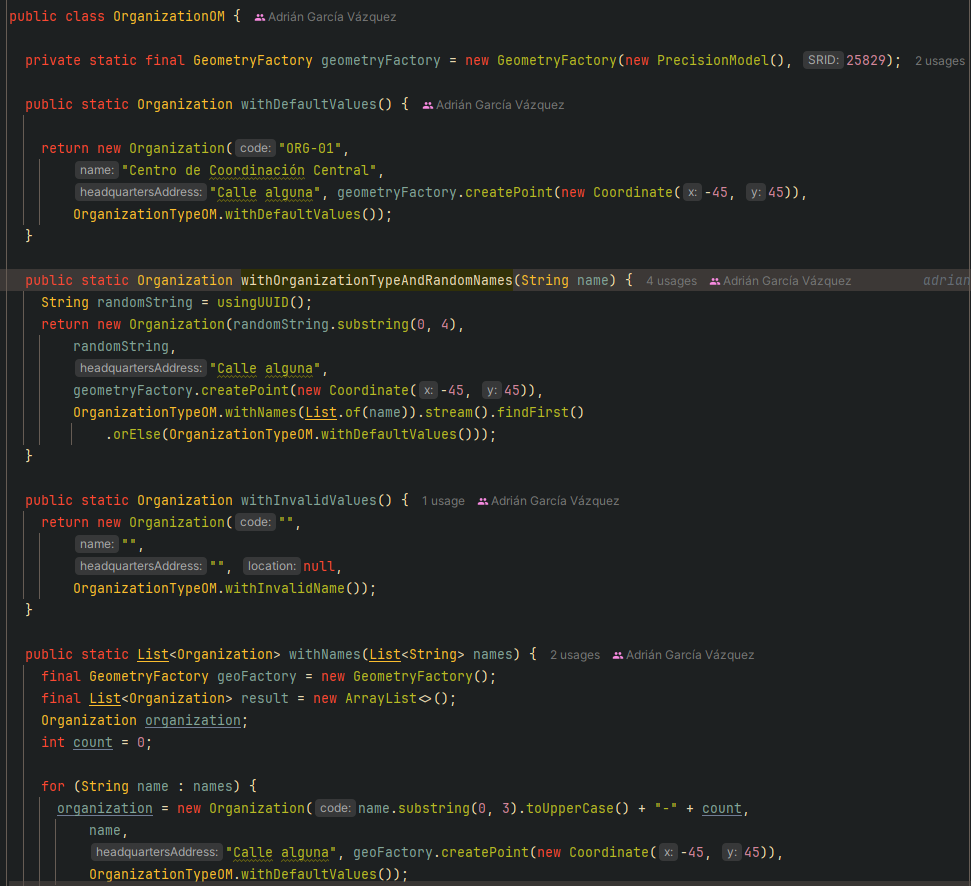
\includegraphics[width=\textwidth]{imaxes/organizacion-om.png}
  \caption{Código de una clase que sigue el patrón Object Mother}
  \label{fig:object-mother}
\end{figure}


\subsection{Pruebas de integración}

Las pruebas de integración utilizan Testcontainers con la imagen \textit{postgis/postgis}, que levanta una instancia efímera de PostgreSQL con PostGIS para cada ejecución. La base de datos se inicializa automáticamente con los mismos scripts SQL de creación de tablas, cuadrantes y datos de inicialización que se emplean en desarrollo (\texttt{01\_create\_tables.sql}, \texttt{02\_init\_quadrants.sql} y \texttt{03\_init\_data.sql}), lo que garantiza que el entorno de pruebas es representativo del real. Todas las pruebas de integración extienden la clase base abstracta \texttt{IntegrationTest}, que configura \texttt{@SpringBootTest}, \texttt{@Transactional} y la inyección automática de propiedades de conexión al contenedor PostgreSQL.

Esta configuración de las pruebas de integración permite validar la lógica de negocio en un entorno realista, con una base de datos real y sin simulaciones. Se han diseñado pruebas para cubrir tanto los flujos normales como los casos de error, incluyendo validaciones de negocio, manejo de excepciones y casos límite. 


\subsection{Cobertura de las pruebas}

En esta imagen \ref{fig:coverage} se muestra la cobertura de las pruebas unitarias e integración del backend. La cobertura es un indicador que aporta confianza pero no garantiza la ausencia de errores, por lo que se ha complementado con un análisis de casos límite y validaciones de negocio en las pruebas de integración. Se ha tratado de alcanzar una cobertura elevada en la capa de servicios mediante una batería de tests de integración que validan tanto los flujos normales como los casos de error, asegurando que la lógica de negocio se comporta correctamente en un entorno realista con una base de datos real. 

\begin{figure}[H]
  \centering
  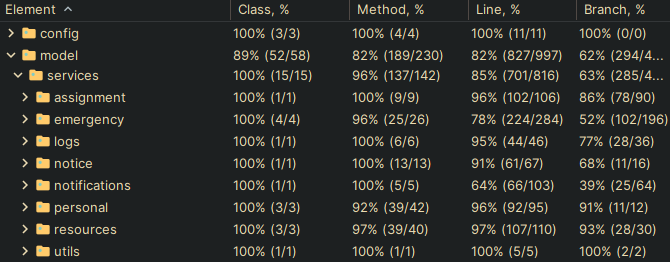
\includegraphics[width=\textwidth]{imaxes/coverage.png}
  \caption{Cobertura de las pruebas del backend}
  \label{fig:coverage}
\end{figure}

\section{Frontend}

Para el frontend se ha adoptado una estrategia de pruebas automatizadas centrada en dos niveles: la lógica pura de la aplicación (funciones de validación, transformación de coordenadas y reductores de estado) y el renderizado de componentes clave. 

Las pruebas se han implementado con Vitest, el ejecutor de tests nativo de Vite. Para el renderizado de componentes se ha empleado React Testing Library, que fomenta pruebas centradas en el comportamiento observable desde la perspectiva del usuario en lugar de detalles de implementación interna.

Se han creado tests distribuidos en las siguientes categorías:

\begin{itemize}
  \item \textbf{Lógica pura:} funciones de validación de formularios (email, teléfono, DNI), formateo de fechas y transformación de coordenadas geográficas a UTM (y viceversa). Estos tests verifican la corrección de la lógica de negocio en el frontend sin necesidad de montar componentes ni depender del navegador, lo que los hace extremadamente rápidos y fiables.
  \item \textbf{Reductores de estado:} pruebas sobre los slices de Redux (\texttt{LoginSlice}, \texttt{themeSlice}) que validan el estado inicial, las transiciones de estado y los selectores.
  \item \textbf{Componentes de interfaz:} renderizado de componentes clave como \texttt{EmergencyTypeIcon} (mapeo de nombres de emergencia a iconos), \texttt{BackButton}, \texttt{NotFoundPage} y \texttt{TeamNotFoundPage}. Estos tests verifican que los componentes se renderizan sin errores, que muestran los elementos esperados (iconos, enlaces, imágenes) y que responden correctamente a las propiedades recibidas.
\end{itemize}

La siguiente imagen \ref{fig:vitest} muestra la ejecución completa de los tests del frontend con Vitest:

\begin{figure}[H]
  \centering
  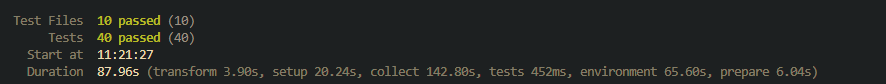
\includegraphics[width=\textwidth]{imaxes/vitest.png}
  \caption{Ejecución de los tests del frontend con Vitest}
  \label{fig:vitest}
\end{figure}

Esta batería de tests automatizados aporta tres beneficios principales. En primer lugar, permite detectar de forma temprana regresiones en la lógica de validación y formateo, que son propensas a errores silenciosos. En segundo lugar, garantiza que los componentes críticos se renderizan correctamente tras cambios en las dependencias o en la estructura del código. Por último, al ejecutarse con Vitest, se integran en el flujo de desarrollo con una ejecución rápida que no interrumpe el trabajo del desarrollador.

Además de las pruebas automatizadas, se ha complementado la validación con un plan de pruebas manuales exhaustivas de la interfaz, que permiten validar la experiencia de usuario, la usabilidad y el comportamiento visual en diferentes dispositivos y navegadores. Dado que el frontend presenta una interfaz gráfica compleja con mapas interactivos y componentes dinámicos, las pruebas manuales cubren aspectos que las pruebas automatizadas no alcanzan, como la correcta visualización del mapa, la respuesta a eventos de usuario y la navegación entre pantallas.

\section{Aplicación Android}


 \chapter{Conclusiones y futuras líneas de trabajo}
\label{chap:conclusions}

\lettrine{D}{erradeiro} capítulo da memoria, onde se presentará a
situación final do traballo, as leccións aprendidas, a relación coas
competencias da titulación en xeral e a mención en particular,
posibles liñas futuras, (no caso de \acrshort{tfm}, carácter profesional del mesmo)\dots

\section{Conclusiones}
\label{sec:conclusions}

\section{Aprendizajes}
\label{sec:aprendizajes}

\section{Futuras líneas de trabajo}
\label{sec:futuro}


 %%%%%%%%%%%%%%%%%%%%%%%%%%%%%%%%%%%%%%%%
 % Apéndices, glosarios e bibliografía  %
 %%%%%%%%%%%%%%%%%%%%%%%%%%%%%%%%%%%%%%%%

 \appendix
 \appendixpage
 \chapter{Material adicional}
\label{chap:adicional}

\lettrine{E}{xemplo} de capítulo con formato de apéndice, onde se pode
incluír material adicional que non teña cabida no corpo principal do
documento, suxeito á limitación de 80 páxinas establecida no
regulamento de TFGs.

\section{Instalación del Software}
\label{sec:instalacion}

\section{Manual de usuario}
\label{sec:manualusuario}

{\color{red} Introducción al layout general de la aplicación, y subapartados para cada una de las secciones principales, para que sea más sencillo de consultar / comprender. }

%\include{anexos/...}

 \printglossary[type=\acronymtype,title=\nomeglosarioacronimos]
 \printglossary[title=\nomeglosariotermos]

 \bibliographystyle{IEEEtranN}
 \bibliography{\bibconfig,bibliografia/bibliografia}
 \clearpage
 

\end{document}

%%%%%%%%%%%%%%%%%%%%%%%%%%%%%%%%%%%%%%%%%%%%%%%%%%%%%%%%%%%%%%%%%%%%%%%%%%%%%%%%
